\documentclass[aspectratio=169]{beamer}
\usetheme{metropolis}
\metroset{block=fill}

\usepackage{newpxtext}
\usepackage{newpxmath}

\usepackage{amsmath}
\usepackage{graphicx}
\usepackage{physics}
\usepackage{ragged2e}
\usepackage{filecontents}
\usepackage{siunitx}

\usepackage{pgfplots}
\pgfplotsset{width=\textwidth, height=0.494427\textwidth}


\usepackage{tikz}
\usepackage{mathtools}
\usetikzlibrary{positioning, shapes.geometric, arrows, arrows.meta, spy}
\usepgfplotslibrary{colorbrewer}

\usefonttheme{serif}

\title{Optically-Active Media}
\subtitle{The QuEST for light-matter models}
\date{December 20, 2017}
\author{Connor Glosser}
\institute{Michigan State University}

\newcommand{\oper}[1]{\mathcal{#1}}
\newcommand{\rwoper}[1]{\tilde{\mathcal{#1}}}
\newcommand{\outerprod}[2]{#1 \! \otimes \! #2}

\begin{document}

\maketitle

\section{About me}

\begin{frame}
  \vspace{0.7cm}
  \begin{columns}[c]
    \column{0.5\textwidth}
      \hfill \includegraphics[width=0.8\textwidth]{figures/coding.jpg} \\ \vspace{0.6cm}
      \hfill \includegraphics[width=0.8\textwidth]{figures/collaboration.jpg}

    \column{0.5\textwidth}
      \includegraphics[width=0.8\textwidth]{figures/strava_cropped.jpg} \vspace{0.6cm}
      \includegraphics[width=0.8\textwidth]{figures/dnd.jpg}
  \end{columns}
\end{frame}

\begin{frame}{Things I've worked on}
  \begin{itemize}
    \item Radiation models (particularly quantum optics: QuEST)
      \begin{itemize}
        \item Rank-deficient fast methods, performance optimization, tree codes, FFTs, GPUs
      \end{itemize}
    \item Hydrocarbon deposition molecular dynamics (REBO)
    \item Nanostructure inverse problem/structure reconstruction (Tribond)
    \item Computational physics education
      \begin{itemize}
        \item \textbf{I}nternational \textbf{C}ourse in \textbf{C}omputational \textbf{P}hysics
        \item Course development, teaching assistantships
        \item Introductory workshops (highschool and college level)
      \end{itemize}
  \end{itemize}
\end{frame}

\section{Making an algorithm}

\begin{frame}
  \vspace{-1cm}
  \begin{columns}
    \begin{column}{0.25\textwidth}
      \begin{center}
        Photovoltaics
      \end{center}
    \end{column}

    \begin{column}{0.25\textwidth}
      \begin{center}
        Next-gen displays
      \end{center}
    \end{column}

    \begin{column}{0.25\textwidth}
      \begin{center}
        Biological contrast
      \end{center}
    \end{column}

    \begin{column}{0.25\textwidth}
      \begin{center}
        Quantum computing
      \end{center}
    \end{column}

  \end{columns}

  \begin{columns}
    \begin{column}{0.25\textwidth}
      \begin{figure}
        \includegraphics[width=\textwidth]{figures/devices/quantum_dot_solar_cell.jpg}
      \end{figure}
    \end{column}

    \begin{column}{0.25\textwidth}
      \begin{figure}
        \includegraphics[width=\textwidth]{figures/devices/quantum_dot_tv.jpg}
      \end{figure}
    \end{column}

    \begin{column}{0.25\textwidth}
      \begin{figure}
        \vspace{-1.2em}
        \includegraphics[width=\textwidth, height=0.4\textheight]{figures/devices/contrast.jpg}
      \end{figure}
    \end{column}

    \begin{column}{0.25\textwidth}
      \begin{figure}
        \includegraphics[width=\textwidth]{figures/devices/quantum_computer.jpg}
      \end{figure}
    \end{column}
  \end{columns}
\end{frame}

\begin{frame}
  \begin{center}
    \includegraphics[width=0.3\textwidth]{figures/einstein_tongue.jpg}
    \hspace{0.1cm}
    \includegraphics[width=0.3\textwidth]{figures/tesla_chair.jpg}
  \end{center}
\end{frame}

\begin{frame}{Simulated quantum dot = two-level system}
  \begin{columns}[c]
    \column{0.3\textwidth}
      \centering
      \input{figures/bloch_sphere}

    \column{0.7\textwidth}
      \begin{itemize}
        \item ``Artifical atoms'' (tuneable spectrum)
        \item Two-level quantum state: $\ket*{\psi} = \alpha \ket{0} + \beta \ket{1}$
        \item $\Delta \mathcal{E} \sim$ optical frequencies; radius $\ll \lambda$
        \item Dynamical absorbtion and emission
      \end{itemize}

      \begin{block}{Liouville equation}
        \begin{equation*}
          \dv{\hat{\rho}}{t} = -\frac{i}{\hbar}\commutator{\hat{\mathcal{H}}}{\hat{\rho}} - \hat{\mathcal{D}}\qty[\hat{\rho}]; \quad \hat{\rho} = \dyad{\psi}{\psi}
        \end{equation*}
        \hfill {\tiny(mixed-state analogue of Schr\"odinger equation)}
      \end{block}
  \end{columns}
\end{frame}

\begin{frame}
  \begin{columns}
    \begin{column}{0.5\textwidth}
        \begin{equation*}
          \dv{\hat{\rho}}{t} = \frac{-i}{\hbar} \commutator{\hat{\mathcal{H}}(t)}{\hat{\rho}} - \hat{\mathcal{D}}\qty[\hat{\rho}]
        \end{equation*}
        \begin{itemize}
          \item Density matrix representation
          \item $\hat{\mathcal{D}}[\hat{\rho}]$ (phenomenologically) incorporates decay and decoherence
          \item Rabi oscillations
          \item One wavefunction/dot
            \begin{itemize}
              \item No universal wavefunction
              \item \emph{Classical} electromagnetic propagation
            \end{itemize}
          \item Exponentially-fitted predictor/corrector
        \end{itemize}
    \end{column}
    \begin{column}{0.5\textwidth}
      \begin{filecontents}{example_bloch.dat}
0.                       0.                        0.                       -1.
0.004887585532746823   0.00009212990552802263    -0.000615646483982036    -0.9999998013063441
0.009775171065493646   0.0003676317912202054     -0.0012010282914746977   -0.9999992013693156
0.01466275659824047    0.00081913688170754       -0.0017152061870508778   -0.9999981788407986
0.019550342130987292   0.0014311451589153646     -0.0021188310912026655   -0.9999967116108025
0.024437927663734115   0.0021803630521431776     -0.002375645903243931    -0.9999947767125574
0.02932551319648094    0.0030362691713231678     -0.002453915675475679    -0.9999923503031307
0.03421309872922776    0.00396198361875489       -0.002327837131421285    -0.9999894076291549
0.039100684261974585   0.004915334014317273      -0.00197864418685883     -0.999985922995586
0.04398826979472141    0.005850155851215669      -0.0013956438469188233   -0.9999818697425832
0.04887585532746823    0.006717762136212471      -0.0005769432294939089   -0.9999772202077034
0.05376344086021505    0.007468556146095187      0.0004699136308808023    -0.9999719456867673
0.05865102639296188    0.008053743553067856      0.0017279121689583606    -0.9999660164265143
0.0635386119257087     0.008427070017187751      0.0031705511003610855    -0.9999594015750168
0.06842619745845552    0.008546547534876265      0.004762230519002424     -0.9999520691318996
0.07331378299120235    0.008376161917972373      0.006458938650232708     -0.9999439859262674
0.07820136852394917    0.007887447376718794      0.00820924886489589      -0.9999351175847436
0.08308895405669599    0.007060882235766189      0.009955621121639334     -0.9999254284848135
0.08797653958944282    0.005887044286284817      0.011635929386712191     -0.9999148817212796
0.09286412512218964    0.0043676602136004695     0.013185201723715945     -0.9999034390542588
0.09775171065493646    0.0025159519705781528     0.014537537172323619     -0.9998910608997763
0.10263929618768328    0.00035722952718118665    0.01562811301246128      -0.9998777062514802
0.1075268817204301     -0.0020711225003983372    0.01639539551064916      -0.9998633326412951
0.11241446725317693    -0.004720263085996062     0.016783230604284795     -0.9998478961058885
0.11730205278592375    -0.007530665424061154     0.016742829803075277     -0.9998313511498157
0.12218963831867058    -0.010433167805171891     0.016234720289108856     -0.9998136506959173
0.1270772238514174     -0.013350349256892281     0.015230758604422844     -0.9997947460021945
0.13196480938416422    -0.016198500118158647     0.01371555629924374      -0.999774586639562
0.13685239491691105    -0.018889714228689077     0.011687616528659558     -0.9997531204498735
0.14173998044965787    -0.02133410653054211      0.009160230014628349     -0.9997302934949316
0.1466275659824047     -0.02344231056476244      0.006162243088186926     -0.9997060499785847
0.15151515151515152    -0.025128191231926146     0.0027382105760085837    -0.9996803321857807
0.15640273704789834    -0.02631147110801985      -0.001052165619945122    -0.999653080453989
0.16129032258064516    -0.026920257247005357     -0.005134788300382488    -0.9996242331189525
0.16617790811339198    -0.02689358105365004      -0.009422252128168414    -0.9995937264460744
0.1710654936461388     -0.02618403642691218      -0.013815334063951275    -0.9995614945343392
0.17595307917888563    -0.024759737394905404     -0.018205286455350727    -0.9995274692852625
0.18084066471163245    -0.02260598147408562      -0.022476268809361592    -0.9994915803514248
0.18572825024437928    -0.019726641826210405     -0.026507978358138642    -0.9994537550713504
0.1906158357771261     -0.01614547083891873      -0.030178647578586657    -0.9994139183665787
0.19550342130987292    -0.011906594355624878     -0.033368375126711855    -0.9993719926726355
0.20039100684261972    -0.007074195652663397     -0.03596243503484473     -0.9993278979017498
0.20527859237536657    -0.0017319575826607778    -0.03785450005988514     -0.9992815513742617
0.2101661779081134     0.00401788428509731       -0.038949960827707845    -0.9992328677287885
0.2150537634408602     0.010056000162224075      -0.03916939085588829     -0.9991817588044863
0.219941348973607      0.01624850422028841       -0.03845128700964907     -0.9991281336060736
0.22482893450635386    0.022449657966167796      -0.03675451031082787     -0.9990718982376254
0.2297165200391007     0.02850487516417199       -0.034060437944687404    -0.9990129558201495
0.2346041055718475     0.03425419057375318       -0.03037509537976885     -0.9989512063585914
0.2394916911045943     0.03953627038834251       -0.025730254039708446    -0.9988865466649562
0.24437927663734115    0.04419250394582606       -0.02018363775419546     -0.9988188703097935
0.249266862170088      0.048071042392305266      -0.01381881631568288     -0.9987480675365302
0.2541544477028348     0.05103105474318558       -0.006744674504413299    -0.9986740251445752
0.2590420332355816     0.05294720370908772       0.000905779617170842     -0.9985966263478278
0.26392961876832845    0.05371343408035044       0.008978019013477612     -0.9985157507353782
0.2688172043010753     0.053246456200609575      0.01729880556179337      -0.9984312741872977
0.2737047898338221     0.051488952188961906      0.02567943208219103      -0.9983430687708815
0.2785923753665689     0.04841286451070309       0.033919528341989025     -0.9982510025714246
0.28347996089931574    0.04402142092948396       0.0418117384172769       -0.9981549396088745
0.2883675464320626     0.03835021839646214       0.04914661197462381      -0.9980547397749824
0.2932551319648094     0.03146790622453881       0.0557175084817501       -0.9979502587274729
0.2981427174975562     0.023476446195302696      0.061325878042417896     -0.9978413477390359
0.30303030303030303    0.01451051276455863       0.06578688565440435      -0.997727853531195
0.30791788856304987    0.004735120735712036      0.06893449356308576      -0.9976096182297095
0.31280547409579668    -0.00565700621048084      0.0706262360241722       -0.9974864792590507
0.31769305962854348    -0.016448656477663234     0.07074777600493765      -0.9973582692125007
0.32258064516129032    -0.027402013340341303     0.0692176808857138       -0.9972248156402872
0.32746823069403717    -0.03826388433099305      0.06599074649561221      -0.9970859409620931
0.33235581622678397    -0.048771291501069264     0.061060370817783045     -0.9969414623862336
0.33724340175953077    -0.058657189166912004     0.05446043292174599      -0.9967911917803743
0.3421309872922776     -0.06765674583792702      0.046266806557511114     -0.9966349354783022
0.34701857282502446    -0.07551417793378198      0.0365977631628225       -0.9964724940897086
0.35190615835777126    -0.08198931026369266      0.025612256441556895     -0.9963036624489755
0.35679374389051806    -0.08686383582940757      0.013507868425445695     -0.9961282294850158
0.3616813294232649     -0.08994748214739845      0.0005180043150411588    -0.9959459780595842
0.36656891495601175    -0.09108456656167696      -0.013091668330835839    -0.9957566847068327
0.37145650048875855    -0.09015901491525026      -0.027028755052795842    -0.9955601195448989
0.37634408602150535    -0.08709846125057595      -0.040980174810114706    -0.9953560461731711
0.3812316715542522     -0.08187777216608094      -0.05461850377543241     -0.9951442215161876
0.38611925708699904    -0.0745223358456391       -0.06760908197252467     -0.9949243955792761
0.39100684261974585    -0.06510995204784395      -0.07961800905130913     -0.9946963112368349
0.39589442815249265    -0.053770318988069096     -0.09032025566869621     -0.9944597041728732
0.40078201368523945    -0.04068407336129215      -0.09940750370916548     -0.9942143027231846
0.4056695992179863     -0.026080937345625485     -0.10659609601202845     -0.9939598276754029
0.4105571847507331     -0.010237015539230395     -0.11163557861628046     -0.9936959919555186
0.4154447702834799     0.006530643667473171      -0.11431579697822726     -0.993422500542589
0.4203323558162268     0.023870119586221945      -0.11447313548808861     -0.9931390503402665
0.4252199413489736     0.04140123688321975       -0.11199614338527633     -0.9928453299906427
0.4301075268817204     0.05872313260490603       -0.10683113691993865     -0.992541019569609
0.4349951124144672     0.07542322631733112       -0.09898611203983002     -0.9922257903589078
0.439882697947214      0.0910867919670439        -0.08853207574722        -0.9918993047766312
0.4447702834799609     0.10530632976856524       -0.0756037931840526      -0.9915612161894612
0.4496578690127077     0.11769133260945491       -0.06039955526387685     -0.9912111686673312
0.4545454545454545     0.12787888877295914       -0.04317998933162643     -0.9908487966153646
0.4594330400782014     0.13554317615135994       -0.024263295952927443    -0.9904737246963866
0.4643206256109482     0.14040420277592644       -0.004019755322283502    -0.9900855676696085
0.469208211143695      0.1422358992363621        0.017134664105759586     -0.9896839301585107
0.4740957966764418     0.14087482176003546       0.03874565669246184      -0.989268406233203
0.4789833822091886     0.13622553643907334       0.06033052372318295      -0.9888385794510826
0.4838709677419355     0.12826570912254479       0.08138824383314511      -0.9883940223971918
0.4887585532746823     0.11704946395567677       0.10141056818853961      -0.9879342966412755
0.4936461388074291     0.10270901961549943       0.11989370588978897      -0.9874589523382437
0.498533724340176      0.08545456843748747       0.1363503322307596       -0.9869675281046181
0.5034213098729228     0.06557215280710608       0.15032155132739386      -0.9864595507240682
0.5083088954056696     0.04342046012396805       0.16138921991663763      -0.9859345348271574
0.5131964809384164     0.01942410007829247       0.16918664357749458      -0.9853919827705052
0.5180840664711632     -0.00593330773487457      0.17340923633426988      -0.9848313843343081
0.5229716520039101     -0.03211821577870148      0.17382398271300223      -0.9842522165308367
0.5278592375366569     -0.058557671531926106     0.17027804994292237      -0.9836539431292136
0.5327468230694037     -0.08465155107052044      0.1627050811171482       -0.9830360145885919
0.5376344086021506     -0.10978567799390503      0.15112966220775076      -0.9823978677245019
0.5425219941348974     -0.13334554286601843      0.13567002145688092      -0.9817389254818647
0.5474095796676442     -0.15473051079941466      0.11653868662715838      -0.9810585966610896
0.552297165200391      -0.1733682651769742       0.09404102643920144      -0.9803562756156639
0.5571847507331378     -0.18872961226495155      0.06857208977951539      -0.979631341921149
0.5620723362658847     -0.20034242813862724      0.04061012097841496      -0.9788831600949792
0.5669599217986315     -0.2078043384781272       0.010707931548656003     -0.9781110794187756
0.5718475073313783     -0.21079433394642794      -0.020517147660509487    -0.9773144336578657
0.5767350928641252     -0.20908309109880557      -0.05239507417599767     -0.9764925407644511
0.581622678396872      -0.20254255032775104      -0.08421659461372542     -0.9756447024382157
0.5865102639296188     -0.19115222991411782      -0.11524882187748964     -0.9747702038946678
0.5913978494623656     -0.17500271597687767      -0.14475164392718276     -0.9738683136651572
0.5962854349951124     -0.15429733120671835      -0.17199437324939376     -0.9729382833144745
0.6011730205278593     -0.12935142629492266      -0.1962727542037305      -0.9719793471480126
0.6060606060606061     -0.10058977180959187      -0.21692664529564448     -0.9709907217824221
0.6109481915933529     -0.06854038324760531      -0.23335727974365345     -0.9699716058299505
0.61583577712609975    -0.033824831337575315     -0.24504283894645218     -0.9689211797419435
0.62072336265884655    0.002852904421073617      -0.2515528569770466      -0.9678386055237244
0.62561094819159335    0.040719679208437685      -0.2525610965866256      -0.9667230264411306
0.63049853372434015    0.07894841627925414       -0.24785731167145858     -0.9655735666207578
0.63538611925708696    0.11667563978447004       -0.23735677799774443     -0.9643893306534157
0.6402737047898338     0.15302084442873692       -0.22110531056900834     -0.9631694034712074
0.64516129032258064    0.18710607938962667       -0.19928226697885673     -0.9619128500763806
0.65004887585532745    0.21807597536378992       -0.17220084342429295     -0.9606187152519343
0.6549364613880743     0.24511831356161382       -0.14030581017995003     -0.959286023200492
0.6598240469208211     0.2674850877062561        -0.10416842483425345     -0.9579137770866304
0.6647116324535679     0.2845116134439786        -0.06447601880529398     -0.9565009589290007
0.6695992179863147     0.2956341859212385        -0.02201964874583531     -0.9550465293641516
0.6744868035190615     0.30040608111870426       0.02232055207248977      -0.9535494273683894
0.6793743890518084     0.2985118268650694        0.06759243683410861      -0.9520085699397963
0.6842619745845552     0.2897802209964501        0.11279133157232266      -0.9504228516162446
0.689149560117302      0.27419198732398536       0.156882355701724        -0.9487911443546027
0.6940371456500489     0.25188431595013555       0.19882340771337806      -0.9471122973549522
0.6989247311827957     0.22315258823101825       0.2375885648533345       -0.9453851368043078
0.7038123167155425     0.18844882467818325       0.2721919636054234       -0.9436084656043596
0.7086999022482893     0.14837752648522826       0.30171266412400605      -0.9417810629111013
0.7135874877810361     0.10368568699289363       0.3253181668559882       -0.9399016839749813
0.718475073313783      0.055249013171743126      0.3422858101406061       -0.93796906004954
0.7233626588465298     0.004055934395228222      0.3520224377313621       -0.9359818981721729
0.7282502443792766     -0.048811295384316236     0.3540818964639185       -0.9339388809431077
0.7331378299120235     -0.10219820398104422      0.34818123644565696      -0.9318386661302362
0.7380254154447703     -0.1549030791907436       0.3342125146317741       -0.9296798864604631
0.7429130009775171     -0.20570382446085064      0.3122491703009045       -0.927461149628184
0.7478005865102639     -0.2533850865316899       0.28254959151519793      -0.9251810381346511
0.7526881720430107     -0.2967659669855437       0.2455568299272872       -0.9228381091281879
0.7575757575757576     -0.3347286524288011       0.2018950744893733       -0.9204308941117566
0.7624633431085044     -0.3662470169952153       0.15236121512760822      -0.917957898698386
0.7673509286412512     -0.3904124253750524       0.09790979377630926      -0.9154176027236716
0.7722385141739981     -0.4064576059653264       0.03963564631160614      -0.9128084601725027
0.7771260997067449     -0.41377811545951554      -0.02124677132341753     -0.9101288990965216
0.7820136852394917     -0.41195170944490095      -0.08342728269403689     -0.907377321452723
0.7869012707722386     -0.40075513372157767      -0.1455273627320828      -0.9045521028633233
0.7917888563049853     -0.3801733164902316       -0.20613102912148148     -0.9016515928240594
0.7966764418377322     -0.3504050653819406       -0.2638161617722001      -0.8986741147546102
0.8015640273704789     -0.3118646002136097       -0.3171864781927488      -0.8956179660163577
0.8064516129032258     -0.265178794187745        -0.364904210219711       -0.8924814178996987
0.8113391984359727     -0.21118054712829154      -0.40572391681809206     -0.8892627154575009
0.8162267839687194     -0.15089358335564687      -0.43852362997517824     -0.8859600777907236
0.8211143695014663     -0.0855134743993869       -0.46233346119143454     -0.882571698265532
0.8260019550342132     -0.016385293312184412     -0.476361669286466       -0.8790957446606368
0.8308895405669599     0.055022589853874405      -0.48001783060887077     -0.8755303593187371
0.8357771260997068     0.12714837609890217       -0.47293429039231377     -0.8718736591332835
0.8406647116324537     0.19837134766531958       -0.4549800594131648      -0.8681237359037284
0.8455522971652004     0.2670479823794081        -0.4262687751516495      -0.8642786567592384
0.8504398826979473     0.3315485298224663        -0.38716255081081136     -0.8603364644715364
0.855327468230694      0.39029430697383133       -0.33827061642863165     -0.8562951777929674
0.8602150537634409     0.44179639037085866       -0.2804438867798376      -0.8521527916668982
0.8651026392961877     0.48469311814424054       -0.21476141874678825     -0.8479072776771827
0.8699902248289345     0.5177839879392081        -0.14250960535750903     -0.8435565847062481
0.8748778103616814     0.5400608909755992        -0.06515823474505546     -0.8390986394572902
0.879765395894428      0.5507359724879869        0.01566794096501116      -0.8345313470101751
0.884652981427175      0.5492671329024136        0.09822179784516592      -0.8298525913124681
0.8895405669599218     0.5353782679349801        0.18067138400854857      -0.8250602357832458
0.8944281524926686     0.5090700958176871        0.26114119994056934      -0.8201521242226456
0.8993157380254154     0.4706266779507811        0.33775376571622484      -0.8151260815937719
0.9042033235581623     0.4206161245860829        0.4086720370370077       -0.8099799148369932
0.909090909090909      0.3598859861222066        0.472142905740993        -0.8047114136845889
0.913978494623656      0.28955240281694083       0.5265413974510557       -0.799318351511205
0.9188660801564028     0.21097819454485728       0.5704107119374205       -0.7937984865079246
0.9237536656891495     0.12574714842080673       0.6024991051020727       -0.7881495627773608
0.9286412512218964     0.03563349791161527       0.6217931577304386       -0.782369311455685
0.9335288367546431     -0.05743350651103832      0.6275474173496829       -0.7764554518837722
0.93841642228739       -0.15140994445325595      0.6193111082911982       -0.7704056928157784
0.943304007820137      -0.2441833452799243       0.5969435340718066       -0.7642177338809069
0.9481915933528836     -0.333619816139814        0.560623317635937        -0.7578892670420677
0.9530791788856305     -0.4176118883056913       0.5108516896944335       -0.7514179780810151
0.9579667644183772     -0.4941271888806538       0.44844909581130654      -0.7448015481613286
0.9628543499511241     -0.5612588463002177       0.3745464401004714       -0.7380376554954479
0.967741935483871      -0.6172727486167098       0.29056419517485826      -0.7311239771555379
0.9726295210166177     -0.6606504527740666       0.19818440770722906      -0.7240581909311817
0.9775171065493646     -0.6901283280529125       0.09931823113825326      -0.7168379772370308
0.9824046920821115     -0.7047321643472086       -0.003932243403138467    -0.7094610211129742
0.9872922776148582     -0.7038090194588406       -0.10931737826427054     -0.7019250144192438
0.9921798631476051     -0.6870495887698327       -0.21449000286407668     -0.6942276581083843
0.997067448680352      -0.6545001440707241       -0.3170586360421731      -0.6863666645005086
1.0019550342130987     -0.6065687237240265       -0.4146409720272659      -0.6783397596727996
1.0068426197458456     -0.544023642757551        -0.5049182257593301      -0.6701446859510838
1.0117302052785923     -0.4679857010720205       -0.585691005861359       -0.661779204671278
1.0166177908113392     -0.37991028818161854      -0.6549344356248044      -0.6532410990616934
1.021505376344086      -0.28155717692818266      -0.7108475551653739      -0.6445281769507823
1.0263929618768328     -0.1749560329133832       -0.7518986084528917      -0.6356382736887496
1.0312805474095797     -0.06236566360186222      -0.776865304489405       -0.6265692551898123
1.0361681329423264     0.05377266289085307       -0.784870846719718       -0.6173190212742121
1.0410557184750733     0.17088834727674074       -0.775414134610545       -0.6078855093171938
1.0459433040078202     0.28634066719842843       -0.7483853883755767      -0.5982666974253136
1.0508308895405669     0.39747821509057957       -0.7040751301687486      -0.5884606079178294
1.0557184750733138     0.5016991339320238        -0.6431750443296504      -0.5784653109767196
1.0606060606060607     0.5965122160980925        -0.5667707463152383      -0.568278928577389
1.0654936461388074     0.6795993547741966        -0.47632693321422404     -0.5578996390161757
1.0703812316715543     0.748872167078484         -0.37365661359774305     -0.5473256806514216
1.0752688172043012     0.8025234343173727        -0.26088402131925337     -0.5365553559307918
1.0801564027370479     0.8390732284645704        -0.14040143103848693     -0.5255870356945413
1.0850439882697948     0.8574092106739146        -0.014819250300708223    -0.5144191637171364
1.0899315738025415     0.8568230508155836        0.113090242665973        -0.503050262125544
1.0948191593352884     0.8370320580456486        0.24045691063110963      -0.49147893589452163
1.0997067448680353     0.7981902852970821        0.36437860140112843      -0.4797038773507284
1.104594330400782      0.7408917987825346        0.48198716789607915      -0.46772387115601677
1.1094819159335289     0.6661644250551121        0.5905149868916795       -0.45553779948386114
1.1143695014662756     0.5754560277597417        0.6873631581505479       -0.4431446482535577
1.1192570869990225     0.47060589550614407       0.770166063962552        -0.43054351261658597
1.1241446725317693     0.35380436163490614       0.8368486841114041       -0.4177336018414191
1.129032258064516      0.2275471988045868        0.885678344542301        -0.4047142449659277
1.133919843597263      0.0945826595625761        0.915309674534202        -0.39148489662073316
1.1388074291300098     -0.042148172801913276     0.9248246885336022       -0.37804514393565425
1.1436950146627566     -0.1795788458483104       0.913762069999379        -0.36439471323673817
1.1485826001955034     -0.31458972631256343      0.8821301050362723       -0.35053347522909106
1.1534701857282503     -0.4440796158989243       0.8304118856661993       -0.3364614512451461
1.158357771260997      -0.5650376280267116       0.7595602271927715       -0.3221788196994207
1.163245356793744      -0.6746157620216117       0.6709834327167914       -0.30768592348290125
1.1681329423264906     -0.7702008003794132       0.5665198053588404       -0.2929832779852241
1.1730205278592375     -0.8494773651471044       0.4483946274161905       -0.2780715765603973
1.1779081133919844     -0.9104845539070991       0.3191716377450857       -0.2629516972056183
1.1827956989247311     -0.9516652631935487       0.18169718278317443      -0.2476247095825855
1.187683284457478      -0.9719083876539805       0.03903716096472613      -0.2320918827202516
1.1925708699902247     -0.9705843887787814       -0.10559322541679284     -0.2163546942543299
1.1974584555229716     -0.9475611618616359       -0.24890682081328253     -0.20041483629787663
1.2023460410557185     -0.9032098621100968       -0.3876215965597184      -0.18427422225899565
1.2072336265884652     -0.8384005656066738       -0.5185372867304616      -0.1679349942932263
1.2121212121212121     -0.7544870058679223       -0.6386115454239709      -0.15139953117169658
1.217008797653959      -0.6532833538550377       -0.7450380365085196      -0.13467045915406956
1.2218963831867057     -0.5370162486923872       -0.8353110947571394      -0.11775065541263845
1.2267839687194526     -0.408278781432947        -0.9072899881192337      -0.10064325805528032
1.2316715542521995     -0.26996964886263763      -0.9592519356845135      -0.08335167392644272
1.2365591397849462     -0.1252256793489543       -0.9899361887331289      -0.0658795851397664
1.2414467253176931     0.0226521730790204        -0.9985769870681276      -0.04823095834534067
1.2463343108504398     0.1702774243746248        -0.9849246163874782      -0.03041005188666283
1.2512218963831867     0.3142593062620826        -0.949253914733529       -0.012421423452248516
1.2561094819159336     0.45128481033165857       -0.892360196335544       0.0057300613751940545
1.2609970674486803     0.5781982104717458        -0.8155403448957375      0.02403922321816454
1.2658846529814272     0.6920798813742757        -0.720566466927973       0.04250055849383231
1.2707722385141739     0.7903166124999856        -0.6096411760661162      0.06110823402624433
1.2756598240469208     0.8706661894410618        -0.4853458567346046      0.07985607915212235
1.2805474095796677     0.9313127155612149        -0.3505783635211526      0.09873757822605676
1.2854349951124144     0.9709114999753292        -0.20848257443894752     0.11774586372031165
1.2903225806451613     0.9886222969383736        -0.06237153909193963     0.1368737090318195
1.2952101661779082     0.9841298362100541        0.08435383860662185      0.1561135220144082
1.3000977517106549     0.9576520553215303        0.22828862489787696      0.17545733780524198
1.3049853372434018     0.9099332442450607        0.36610796667470674      0.19489681305706075
1.3098729227761487     0.8422250696788126        0.4946491827863021       0.21442321989239252
1.3147605083088954     0.7562543279673125        0.6109898707655823       0.23402743976857365
1.3196480938416423     0.6541785799600263        0.7125199373028156       0.2536999584526354
1.324535679374389      0.5385307691507266        0.7970056397273313       0.27343086055522414
1.3294232649071359     0.4121542271405713        0.8626439460722151       0.2932098250731819
1.3343108504398828     0.2781298536144256        0.9081063459071792       0.3130261203726054
1.3391984359726295     0.13969664174196278       0.9325674980822738       0.33286860219957887
1.3440860215053764     0.00016969970737015783    0.9357258114984431       0.35272570800815795
1.348973607038123      -0.1371451335996876       0.9178066015409245       0.3725854546113553
1.35386119257087       -0.26903545013034635      0.8795520418257854       0.3924354363036011
1.3587487781036169     -0.3924635979393679       0.8221978919935782       0.4122628227166519
1.3636363636363636     -0.5046430961548866       0.7474373802509464       0.43205435772078793
1.3685239491691105     -0.6031080723217233       0.6573731716554457       0.45179635874603263
1.3734115347018573     -0.6857738791628526       0.5544587372985986       0.4714747166940057
1.378299120234604      -0.7509874132846539       0.441430753362239        0.4910748965511646
1.383186705767351      -0.7975669336794623       0.321234056296157        0.5105819375975906
1.3880742913000978     -0.8248234531932694       0.1969406395955629       0.5299804588187594
1.3929618768328446     -0.8325754706504774       0.07166765118989266      0.5492546591045488
1.3978494623655914     -0.8211459185608886       -0.05150657671318253     0.5683883222820004
1.4027370478983382     -0.7913461435711777       -0.16962445964281042     0.5873648211073047
1.407624633431085      -0.7444464644196381       -0.279927047162489       0.6061671236903501
1.412512218963832      -0.6821342073770491       -0.3799256793562998      0.6247777994684318
1.4173998044965786     -0.6064605274323389       -0.46746541440181205     0.6431790273310971
1.4222873900293255     -0.51977791679166         -0.5407795326762689      0.6613526029484524
1.4271749755620722     -0.4246676798215273       -0.5985271293345203      0.6792799521351508
1.4320625610948191     -0.3238662629333537       -0.6398285785613488      0.6969421366788875
1.436950146627566      -0.2201830103981117       -0.6642779543035461      0.7143198689527189
1.4418377321603127     -0.11641939895516559      -0.6719440925150455      0.7313935254418724
1.4467253176930596     -0.015289071344878613     -0.6633600046789888      0.7481431603642262
1.4516129032258065     0.08065920599304398       -0.6394977089312411      0.7645485205356042
1.4565004887585532     0.16911318405422981       -0.6017301598837724      0.780589062558556
1.4613880742913001     0.24805814269213666       -0.5517794048307088      0.7962439721929202
1.466275659824047      0.31583157685277957       -0.4916591832044114      0.8114921824357709
1.4711632453567937     0.37116471061099193       -0.42360662020653206     0.8263123947425234
1.4760508308895406     0.4132118122547257        -0.35000856055964574     0.84068310133564
1.4809384164222873     0.44156608546585563       -0.27332419184208523     0.8545826087502341
1.4858260019550342     0.4562616938500795        -0.19600636152550016     0.8679890629994542
1.4907135874877811     0.45776231095022574       -0.12042379994662841     0.8808804759177316
1.4956011730205278     0.44693424716122526       -0.04878794124489245     0.893234753508929
1.5004887585532747     0.4250103866629635        0.016915797413680073     0.905029725204747
1.5053763440860214     0.3935401880681814        0.07498802618594148      0.9162431746649189
1.5102639296187683     0.3543304047554445        0.1240655998129596       0.9268528727396712
1.5151515151515152     0.3093778242374194        0.16315975009089295      0.9368366111886537
1.5200391006842619     0.26079664138355074       0.19168171599667225      0.9461722383027389
1.5249266862170088     0.21074262921786008       0.20945442448874177      0.9548376957098863
1.5298142717497557     0.16133606792490843       0.21671224101420777      0.9628110575319253
1.5347018572825024     0.11458663894569032       0.21408330746126528      0.970070569611994
1.5395894428152493     0.07232242853381597       0.20256099782353262      0.9765946915842209
1.5444770283479962     0.03612555702218909       0.18346188748813289      0.9823621395929449
1.5493646138807429     0.0072765720473435686     0.15837271509600484      0.9873519308905865
1.5542521994134898     -0.013290466422927897     0.12908794162318568      0.9915434294540052
1.5591397849462365     -0.02502064217340768      0.09753996942441032      0.9949163933678793
1.5640273704789834     -0.027757387341870627     0.06572436097422765      0.9974510231190765
1.5689149560117303     -0.021747492175478222     0.0356225786945585       0.9991280115654955
1.573802541544477      -0.007631632468274189     0.009124882278216173     0.9999285947871045
1.5786901270772237     0.01357938285905474       -0.012043958125841135    0.9998346043701002
1.5835777126099706     0.04054196497889989       -0.02639353580824558     0.9988285205926848
1.5884652981427175     0.07162954870738304       -0.032728821657067406    0.996893526771528
1.5933528836754644     0.10499326311347458       -0.030201104864356315    0.9940135644672676
1.5982404692082113     0.13863149350700338       -0.018346956780575796    0.9901733896001896
1.6031280547409578     0.17046603036935667       0.0028863061715654423    0.9853586293064429
1.6080156402737047     0.19842224082181112       0.033129748800119645     0.9795558394682281
1.6129032258064516     0.22051052185864298       0.07159714063883406      0.9727525628025221
1.6177908113391985     0.23490620576955698       0.11710457631903043      0.9649373873855019
1.6226783968719453     0.24002509396792765       0.16810497137506034      0.9561000055047799
1.6275659824046922     0.23459189580498618       0.22273649629403625      0.9462312726925929
1.6324535679374388     0.21769904347866625       0.2788835177104798       0.9353232668184204
1.6373411534701857     0.1888536374429148        0.33424816127735546      0.9233693470825812
1.6422287390029325     0.14801064151566204       0.38643021137211736      0.9103642127693233
1.6471163245356794     0.09559088224810018       0.43301273340569013      0.8963039615919981
1.6520039100684263     0.03248289999729345       0.4716505572524146       0.8811861474691611
1.656891495601173      -0.039971766012548954     0.5001586054954166       0.8650098375544036
1.6617790811339198     -0.12000971670307696      0.5165969947144567       0.8477756683414563
1.6666666666666666     -0.20549254827475386      0.5193498860173777       0.8294859006564139
1.6715542521994135     -0.2939681621660429       0.5071952128513147       0.8101444733438937
1.6764418377321604     -0.38274474691857824      0.47936266693053403      0.789757055447572
1.6813294232649073     -0.46897517751683904      0.4355776703620676       0.7683310966794458
1.686217008797654      -0.5497491734640436       0.37608949396124836      0.7458758759673993
1.6911045943304007     -0.6221902349642762       0.3016821853789531       0.7224025478649462
1.6959921798631476     -0.6835541498246598       0.21366753037681252      0.6979241866031907
1.7008797653958945     -0.7313257418508099       0.11385986845010782      0.6724558275603796
1.7057673509286414     -0.763310520977807        0.004533200390333094     0.6460145059214606
1.710654936461388      -0.7777179988991271       -0.11163836041439999     0.6186192922967537
1.715542521994135      -0.7732336504042175       -0.23165515021782535     0.590291325066832
1.7204301075268817     -0.7490768249928901       -0.3522793411039105      0.5610538392189515
1.7253176930596286     -0.7050423367473898       -0.47013247845524486     0.5309321914395789
1.7302052785923755     -0.641523970448194        -0.5818000957075404      0.49995388122741286
1.735092864125122      -0.5595187227803774       -0.6839400283807286      0.4681485677920195
1.739980449657869      -0.46061123065619064      -0.7733908552048776      0.4355480825047008
1.7448680351906158     -0.34693850341050464      -0.8472768188385462      0.4021864366707679
1.7497556207233627     -0.22113574958544543      -0.9031056272954857      0.36809982439563804
1.7546432062561096     -0.08626474907004718      -0.9388557106417653      0.33332662032165183
1.759530791788856      0.054273155668378134      -0.9530498023657047      0.2979073720177862
1.764418377321603      0.1968368120161459        -0.9448121233118376      0.26188478681092836
1.76930596285435       0.33765463281736424       -0.9139069563239576      0.22530371285484657
1.7741935483870968     0.47294009012002364       -0.8607569960560203      0.18821111424158005
1.7790811339198437     0.5990095515863676        -0.7864405217210757      0.15065603996973442
1.7839687194525906     0.7123985394468771        -0.6926671490310642      0.11268958659511084
1.788856304985337      0.8099724805775589        -0.5817326473494557      0.07436485440113495
1.793743890518084      0.8890281413246698        -0.4564540339896652      0.03573689693980552
1.798631476050831      0.9473822003413687        -0.32008685410334076     -0.003137336191495232
1.8035190615835778     0.9834438003934722        -0.17622719667123773     -0.042199063456477906
1.8084066471163247     0.9962684246158297        -0.028701561100214785    -0.08138774247177327
1.8132942326490712     0.9855910484588991        0.11855184651642892      -0.12064114816818386
1.818181818181818      0.9518372060335107        0.2616064615623558       -0.15989545808601047
1.823069403714565      0.8961113559066922        0.3966712128590905       -0.1990853448486427
1.827956989247312      0.82016262564075          0.520210583263086        -0.2381440759600866
1.8328445747800588     0.7263291828913171        0.6290568947805709       -0.2770036205347762
1.8377321603128056     0.6174628613942563        0.7205112920592456       -0.31559476275607024
1.8426197458455522     0.4968356351274686        0.792428609156554        -0.3538472238104074
1.847507331378299      0.3680322257130024        0.8432841257032876       -0.3916897904610198
1.852394916911046      0.23483199894603707       0.8722195313696013       -0.4290504497596208
1.857282502443793      0.1010841443263043        0.8790663738578437       -0.4658565310577609
1.8621700879765397     -0.02941950679491142      0.8643459089594417       -0.502034854792537
1.8670576735092863     -0.15307001151511312      0.8292461408181097       -0.5375118870462284
1.871945259042033      -0.2665600194455981       0.775574396157021        -0.5722139013954918
1.87683284457478       -0.3669920893877826       0.7056896369444401       -0.6060671463701425
1.881720430107527      -0.4519723924781247       0.6224151712561632       -0.6389980182867993
1.886608015640274      -0.5196863375430485       0.5289353104930019       -0.6709332403081818
1.8914956011730204     -0.5689534983515631       0.42867965059748514      -0.7018000455962944
1.8963831867057673     -0.5992603688286459       0.325198871729341        -0.7315263669971046
1.901270772238514      -0.610766416492704        0.2220370997284011       -0.7600410259905099
1.906158357771261      -0.6042899955865884       0.12260474085532204      -0.7872739328177066
1.911045943304008      -0.5812673174268198       0.030056674317565257     -0.8131562840361285
1.9159335288367545     -0.5436909991861913       -0.05282099966212332     -0.8376207708823857
1.9208211143695014     -0.49402422856021333      -0.12370613327949531     -0.8606017738647562
1.9257086999022482     -0.43510297820092353      -0.1808224196898113      -0.8820355759512021
1.930596285434995      -0.3700218779753126       -0.22300102786007614     -0.9018605788062752
1.935483870967742      -0.3020095609207284       -0.24971250674163353     -0.9200174955077881
1.940371456500489      -0.23430171062189076      -0.2610812014389107      -0.9364495682436751
1.9452590420332354     -0.17001289151817625      -0.25787153458293727     -0.9511027741721542
1.9501466275659823     -0.11201343397301788      -0.24145020555103383     -0.9639260320163417
1.9550342130987292     -0.06281560023483007      -0.21372528814109898     -0.9748714079817523
1.959921798631476      -0.02447363425530836      -0.17706366395351253     -0.9838943184757354
1.964809384164223      0.0014976617477610102     -0.13419015456665767     -0.9909537258943049
1.9696969696969695     0.014183388827826576      -0.08807273716030052     -0.9960123320991964
1.9745845552297164     0.013305451787192115      -0.04179782499297051     -0.9990367667141112
1.9794721407624633     -0.0007657155381278541    0.0015596494000755488    -0.9999977696102679
1.9843597262952102     -0.027025245273572234     0.03906635063720612      -0.9988703666711848
1.989247311827957      -0.0638733891263513       0.06805580869537872      -0.9956340382042971
1.994134897360704      -0.10917901893585462      0.08624423835732617      -0.9902728819016988
1.9990224828934505     -0.1603656997822577       0.09183185479295408      -0.9827757638504715
2.0039100684261974     -0.21451655591942484      0.08358507262269144      -0.97313645695368
2.0087976539589443     -0.2684936179822391       0.06089692836182247      -0.9613537710850732
2.0136852394916912     -0.31906743236769747      0.023822964956892234     -0.9474316719116599
2.018572825024438      -0.3630519648037748       -0.026909114326965626    -0.9313793875281422
2.0234604105571846     -0.3974395612649359       -0.08991670418404286     -0.9132115021712673
2.0283479960899315     -0.4195306849836805       -0.16320607079356997     -0.8929480366428246
2.0332355816226784     -0.42705365247133725      -0.2442410939856889      -0.870614517804552
2.0381231671554253     -0.4182688229978225       -0.33003558108872655     -0.8462420280217178
2.043010752688172      -0.3920527184850553       -0.41726490715138        -0.8198672376644293
2.0478983382209187     -0.3479591824425792       -0.5023926778429452      -0.7915324239213304
2.0527859237536656     -0.28625469328705383      -0.5818079065823012      -0.7612854729379703
2.0576735092864125     -0.2079260943510115       -0.651967470358592       -0.7291798647410448
2.0625610948191594     -0.11466006354514961      -0.7095383357333067      -0.6952746405042733
2.0674486803519063     -0.008794809638609666     -0.7515340263723399      -0.6596343523335616
2.0723362658846528     0.10675440540625897       -0.7754403477266314      -0.6223289977082217
2.0772238514173997     0.2285944246358049        -0.7793243295435649      -0.5834339289557827
2.0821114369501466     0.35297330210495037       -0.7619220004959341      -0.5430297443537583
2.0869990224828935     0.4759150111815242        -0.7227018422525271      -0.5012021621938693
2.0918866080156404     0.5933649285906134        -0.6619009598137748      -0.4580418757522126
2.0967741935483872     0.7013405723487321        -0.5805322115836473      -0.41364438914771046
2.1016617790811338     0.796081801006712         -0.48036165858262425     -0.36810983415433135
2.1065493646138807     0.874194703711278         -0.36385695598034923     -0.32154276879632265
2.1114369501466276     0.9327839560476732        -0.23410832387961544     -0.2740519589209207
2.1163245356793745     0.9695671801148427        -0.09472378603214104     -0.2257501359134524
2.1212121212121213     0.982967075929458         0.050296133132415016     -0.1767537381957915
2.126099706744868      0.9721779053057699        0.19669983371843944      -0.12718263631275917
2.1309872922776148     0.9372033431511634        0.3401370354388065       -0.07715984100697065
2.1358748778103617     0.878863955797108         0.4763163389914876       -0.0268111949017593
2.1407624633431085     0.7987737397286044        0.6011618905777667       0.023734951507410486
2.1456500488758554     0.699286528395672         0.7109631684627914       0.07434807831630771
2.1505376344086023     0.5834139033810405        0.802512407524096        0.1248958489663276
2.155425219941349      0.45471665636798697       0.8732229173435061       0.17524447843107727
2.1603128054740958     0.317175342466589         0.9212242065583152       0.22525911182660294
2.1652003910068426     0.1750444624028096        0.9454302780660098       0.27480421369941027
2.1700879765395895     0.03269574255860979       0.9455781581765541       0.3237439671521415
2.1749755620723364     -0.10554342279759621      0.9222349915120344       0.3719426815812484
2.179863147605083      -0.23555006775428328      0.8767732669133841       0.4192652077397222
2.18475073313783       -0.3535579725754623       0.8113150357936793       0.46557735850017645
2.1896383186705767     -0.4562980887015169       0.728648162191282        0.5107463404764075
2.1945259042033236     -0.541114819444638        0.6321125891936545       0.554641174416584
2.1994134897360705     -0.6060618680182451       0.5254699869250231       0.5971331280537389
2.204301075268817      -0.6499725115040533       0.4127556355747525       0.6380961578744098
2.209188660801564      -0.6724901518490699       0.29811828988802974      0.6774073178627168
2.214076246334311      -0.6740765498838808       0.18565814846569798      0.7149472007179085
2.2189638318670577     -0.6559828520264837       0.07926545333113214      0.7506003598121814
2.2238514173998046     -0.6201880991659072       -0.017530752299641846    0.7842557169539836
2.228739002932551      -0.5693104860227131       -0.10169892862995505     0.8158069694127867
2.233626588465298      -0.506492988159865        -0.17082082955612338     0.8451529862194573
2.238514173998045      -0.43526819835532643      -0.22318220529658844     0.872198193667136
2.2434017595307918     -0.35940754313401096      -0.25783552870838383     0.8968529560736558
2.2482893450635387     -0.28276026052967446      -0.2746294823291443      0.9190339305678924
2.2531769305962856     -0.20909045193839199      -0.2742052017924516      0.938664403582396
2.258064516129032      -0.14191830466419592      -0.25796039577921437     0.9556746137114533
2.262952101661779      -0.0843717644444838       -0.2279821715015158      0.9700020555091092
2.267839687194526      -0.03905470926656363      -0.18695129209197492     0.9815917632117296
2.2727272727272728     -0.007936240007282663     -0.13802187500396068     0.9903965815224622
2.2776148582600197     0.007732486280827638      -0.08467987688290209     0.9963774019606765
2.2825024437927662     0.007470153776005243      -0.030587893476405073    0.9995033679155846
2.287390029325513      -0.00841470507068785      0.02057714431728762      0.9997520609924102
2.29227761485826       -0.03883706251689706      0.06528719476285358      0.9971096606120797
2.297165200391007      -0.08198167036009157      0.10032050589178643      0.9915710760332699
2.3020527859237538     -0.13538002768239446      0.1229072987717757       0.9831400585831608
2.3069403714565007     -0.19601675353495066      0.1308568790977407       0.971829275817754
2.3118279569892472     -0.26046016804934885      0.12265940631753197      0.9576603440380866
2.316715542521994      -0.32501051637338246      0.09755970516969605      0.9406638392567578
2.321603128054741      -0.38586052868976106      0.05559957890954595      0.9208792773818864
2.326490713587488      -0.43926173437744387      -0.0023733374507477895   0.8983550629136653
2.3313782991202348     -0.48169003396113225      -0.07473015790686419     0.8731484132328626
2.3362658846529813     -0.5100038388018693       -0.1591193831352173      0.8453252466415058
2.3411534701857282     -0.5215862239719273       -0.2525578344749057      0.8149600237888277
2.346041055718475      -0.5144663526407813       -0.3515479928910067      0.7821355675690272
2.350928641251222      -0.4874150369066954       -0.4522179286451956      0.7469428527416571
2.355816226783969      -0.44001025754049566      -0.5504782502299456      0.7094807647910402
2.3607038123167154     -0.372670305699605        -0.6421897931488787      0.6698558335284137
2.3655913978494623     -0.2866522607013696       -0.7233359606613083      0.6281819364835668
2.370478983382209      -0.18401367704509866      -0.7901910377756214      0.5845799586153549
2.375366568914956      -0.06754185513134359      -0.8394776806981737      0.539177433446799
2.380254154447703      0.059347340856445774      -0.8685074912413129      0.4921081591885436
2.3851417399804495     0.19273730964668234       -0.8752987602707772      0.44351178967341026
2.3900293255131964     0.32835999310246816       -0.8586668419285582      0.39353340392553915
2.3949169110459433     0.4617614174453871        -0.8182834513051788      0.3423230540663705
2.39980449657869       0.5884764160186671        -0.7546992891926166      0.2900352810012681
2.404692082111437      0.704204156895465         -0.6693318479077487      0.23682861747515135
2.409579667644184      0.8049780752758054        -0.5644184525267327      0.1828650753677695
2.4144672531769305     0.8873232993853927        -0.4429360339279176      0.12830961757156928
2.4193548387096774     0.9483953490321444        -0.3084909578467797      0.07332961705370103
2.4242424242424242     0.986095135120113         -0.16518293015459617     0.018094303904731275
2.429130009775171      0.9991524563935262        -0.017447227524955047    -0.03722580178818023
2.434017595307918      0.9871764312097275        0.1301159210760951       -0.09245946060796753
2.4389051808406646     0.9506711667627887        0.27291857706289857      -0.14743528869758685
2.4437927663734114     0.891015618038938         0.4065619802653134       -0.2019823355078955
2.4486803519061583     0.8104084561701005        0.5270058449570602       -0.25593066195629494
2.4535679374389052     0.7117812288242997        0.6307249633323183       -0.30911192332812176
2.458455522971652      0.5986788149082835        0.7148426826791671       -0.36135994220131035
2.463343108504399      0.47511682096289415       0.7772366690515016       -0.41251126965063606
2.4682306940371455     0.345422198123945         0.816616174691121        -0.4624057443371218
2.4731182795698924     0.21406047388163946       0.8325680232348174       -0.5108870569145556
2.4780058651026393     0.0854573865669058        0.8255599625205271       -0.5578032702466212
2.4828934506353862     -0.036176156789749045     0.7969133436500624       -0.6030073496251991
2.487781036168133      -0.1470085066876486       0.7487378745047926       -0.6463576541787683
2.4926686217008796     -0.24373663144604285      0.6838378641575945       -0.6877184334521945
2.4975562072336265     -0.3237122563292701       0.605588413807645        -0.7269602883221099
2.5024437927663734     -0.3850406594553354       0.5177892571471601       -0.7639606174534471
2.5073313782991203     -0.42664686292616005      0.42450162425594307      -0.7986040312607191
2.5122189638318672     -0.44830803018403925      0.32987554748912806      -0.8307827496537393
2.5171065493646137     -0.4506473827113987       0.23797549444778465      -0.8603969428352021
2.5219941348973606     -0.43509690778338345      0.15261045166250853      -0.8873550834122117
2.5268817204301075     -0.40382487808319395      0.07717499708422319      -0.911574255923305
2.5317693059628544     -0.35963220749051195      0.014508536487851054     -0.93298043883186
2.5366568914956013     -0.30582054220872523      -0.0332166143544458      -0.951508699589296
2.5415444770283478     -0.24604476572470607      -0.06458423815704271     -0.9671034406776928
2.5464320625610947     -0.1841476441789464       -0.07898977028621706     -0.9797185921305451
2.5513196480938416     -0.1239876801721185       -0.07665429124499826     -0.9893176950938403
2.5562072336265885     -0.06926852027234326      -0.058610091449812524    -0.9958740313457546
2.5610948191593354     -0.023374859866250715     -0.026649263641042205    -0.9993706893892541
2.5659824046920823     0.010778698707967188      0.016759189712741752     -0.9998006132768331
2.5708699902248288     0.03087702441830381       0.06858349433124754      -0.9971665877381187
2.5757575757575757     0.035307184907573286      0.12536637056717376      -0.991481191573787
2.5806451612903226     0.02323138448343557       0.18337983408807199      -0.9827667239523762
2.5855327468230695     -0.005373246770563743     0.23879158216319363      -0.9710550963730648
2.5904203323558164     -0.049708826314535944     0.28783633295702227      -0.9563877008359927
2.595307917888563      -0.10818678230649634      0.3269855432234668       -0.9388152391490765
2.6001955034213098     -0.1784937296319788       0.35310612793646445      -0.9183974991759675
2.6050830889540567     -0.2576870863184381       0.3636025335327287       -0.8952031138285267
2.6099706744868036     -0.3423175667787302       0.3565365173423948       -0.86930929135996
2.6148582600195504     -0.4285735235563534       0.3307198167076892       -0.8408015188672253
2.6197458455522973     -0.5124416503482001       0.28577684929431035      -0.8097732478160558
2.624633431085044      -0.5898779482933949       0.22217098113713177      -0.7763255302313139
2.6295210166177908     -0.6569796912645293       0.14119560190024502      -0.7405666342702557
2.6344086021505377     -0.7101521374131525       0.04493126505598069      -0.7026116435476258
2.6392961876832845     -0.746263319737564        -0.06383003303632799     -0.6625820353041995
2.6441837732160314     -0.762781320002854        -0.1816899170159045      -0.6206052445970016
2.649071358748778      -0.7578878812866419       -0.30477536929977506     -0.5768142061096618
2.653958944281525      -0.7305609441763796       -0.4288914246098122      -0.5313468684915567
2.6588465298142717     -0.6806257330385143       -0.5496864771840644      -0.48434570455529313
2.6637341153470186     -0.6087718148532223       -0.662824539848451       -0.4359572106615347
2.6686217008797655     -0.5165355089269519       -0.7641576130903209      -0.386331397124752
2.673509286412512      -0.4062487500609536       -0.8498919677597108      -0.3356212724585664
2.678396871945259      -0.28095424553137427      -0.9167410726453737      -0.2839823159044475
2.683284457478006      -0.14429016776822695      -0.96205497751254        -0.2315719422485218
2.6881720430107527     -0.00035481693972451434   -0.9839283122576491      -0.17854897741870546
2.6930596285434996     0.14644948833183907       -0.9812767709657858      -0.12507312826546654
2.697947214076246      0.2915841260273222        -0.9538812971574921      -0.07130445388361246
2.702834799608993      0.4305471421248687        -0.9023979127554362      -0.01740284332792262
2.70772238514174       0.5590444847191557        -0.8283329042813841      0.036472501822317586
2.7126099706744868     0.6731525943351273        -0.7339844835015548      0.09016357488015078
2.7174975562072337     0.7694650519847906        -0.6223528836969986      0.14351406066387568
2.7223851417399806     0.8452214645860291        -0.4970257297615469      0.19636983019160772
2.727272727272727      0.8984054351331386        -0.3620362449954313      0.24857940568057485
2.732160312805474      0.9278159724259027        -0.22170845523455154     0.299994422531979
2.737047898338221      0.9331052855211085        -0.08049073621475147     0.35047007057589086
2.7419354838709678     0.9147828183535736        0.05721414919295334      0.39986551811904497
2.7468230694037147     0.8741854906864536        0.1872158021037967       0.44804431642047055
2.7517106549364612     0.8134155700680782        0.3056930640904204       0.49487478439710864
2.756598240469208      0.7352489212688473        0.4093347893708798       0.5402303709870812
2.761485826001955      0.6430177671514871        0.49545974953730393      0.5839900013805921
2.766373411534702      0.5404713548818083        0.5621059471255416       0.6260383662519455
2.7712609970674488     0.43162493957406733       0.6081001951970274       0.6662662634655983
2.7761485826001957     0.32059561177119383       0.633084176608146        0.7045708273497219
2.7810361681329422     0.21143900230783108       0.6375139072131701       0.7408557805500806
2.785923753665689      0.10798973860697306       0.6226252837031665       0.7750316513558609
2.790811339198436      0.013712768360998627      0.5903687587986215       0.807015962740866
2.795698924731183      -0.068428866466265        0.543316252253887        0.8367334005361656
2.8005865102639298     -0.13608376533686126      0.4845433730760386       0.8641159458079216
2.8054740957966763     -0.18759750692847443      0.41749328194971325      0.8891030019223038
2.8103616813294232     -0.22206290877164483      0.3458261148312806       0.9116414399197641
2.81524926686217       -0.2393462971360604       0.27326358281881524      0.9316856885252682
2.820136852394917      -0.24007765325480107      0.20343124606572896      0.9491977567379101
2.825024437927664      -0.22561037651665622      0.1397069772644698       0.9641472400268993
2.8299120234604104     -0.1979516683198387       0.08508128977808596      0.9765113006359336
2.8347996089931573     -0.15966663657004976      0.0420351050779086       0.9862746247936575
2.8396871945259042     -0.11376022953123954      0.012439784571125382     0.9934293545043551
2.844574780058651      -0.06354199184830812      -0.002516710982642373    0.9979749976860299
2.849462365591398      -0.012479361400179901     -0.002374271337693714    0.9999183110244948
2.8543499511241445     0.035954730319695         0.01258392156824898      0.999273176113996
2.8592375366568914     0.07843348434172595       0.041348977059187796     0.996060435776745
2.8641251221896383     0.11192084896049243       0.08223275494976653      0.9903077216555417
2.869012707722385      0.13380344409975295       0.13294248364343986      0.9820492613475702
2.873900293255132      0.14200451906162792       0.19068012484925884      0.971325668598
2.878787878787879      0.13507543220107457       0.25226234077512977      0.9581837167359761
2.8836754643206255     0.11226108507529173       0.3142561128082469       0.9426760974635935
2.8885630498533724     0.07353657594682979       0.37312442390658423      0.9248611640911765
2.8934506353861193     0.019614981067409165      0.42537633575091877      0.9048026693264228
2.898338220918866      -0.04807669254046225      0.4677151130716838       0.8825694793425
2.903225806451613      -0.1274491390517419       0.4971786886202549       0.8582352878409782
2.9081133919843596     -0.21582982726849065      0.511266821435605        0.8318783171964889
2.9130009775171065     -0.3100655810003309       0.5080499638274603       0.8035810123460749
2.9178885630498533     -0.4066446296857254       0.48625558787577944      0.7734297286173324
2.9227761485826002     -0.5018332477806963       0.4453286503889656       0.7415144141715717
2.927663734115347      -0.5918216044763133       0.3854639070629051       0.7079282886675593
2.932551319648094      -0.6728730549689049       0.3076088196293053       0.6727675188786383
2.9374389051808406     -0.741471007148559        0.21343711172585372      0.6361308929101279
2.9423264907135874     -0.7944577006641843       0.10529409064438158      0.5981194940087922
2.9472140762463343     -0.8291595517255137       -0.013884065534849235    0.5588363750305935
2.9521016617790812     -0.8434942808853907       -0.14067385463295268     0.5183862347207359
2.956989247311828      -0.8360557788757864       -0.27128677433540704     0.47687509674834133
2.9618768328445746     -0.806173553114648        -0.40170567430743814     0.4344099925976072
2.9667644183773215     -0.7539445970520295       -0.5278298870123455      0.3910986491756597
2.9716520039100684     -0.6802361942278884       -0.6456233761210634      0.34704918226692266
2.9765395894428153     -0.5866622157719722       -0.7512615508816415      0.3023697958432968
2.9814271749755622     -0.47552732323971203      -0.8412681900895969      0.2571684897473085
2.9863147605083087     -0.3497506340216527       -0.9126412656303258      0.2115527748708407
2.9912023460410556     -0.21276448158107225      -0.9629602913524129      0.1656293970303381
2.9960899315738025     -0.06839530910507102      -0.990472329581111       0.1195040705257551
3.0009775171065494     0.07926930047082743       -0.9941534549067064      0.07328122156363867
3.0058651026392963     0.22602242496880343       -0.9737435890178185      0.0270637424182628
3.010752688172043      0.36768312876362036       -0.9297536294461736      -0.01904724360761742
3.0156402737047897     0.5002399240190676        -0.8634448534055409      -0.06495260533494807
3.0205278592375366     0.6199871161604275        -0.7767816039408558      -0.11055541563174301
3.0254154447702835     0.72364909600718          -0.672359257515303       -0.1557611504016818
3.0303030303030304     0.8084881992214268        -0.5533103763000083      -0.20047787617850563
3.0351906158357773     0.8723919124803583        -0.42319258686946837     -0.2446164225040963
3.0400782013685238     0.9139381232330819        -0.2858629898614941      -0.28809054747752966
3.0449657869012707     0.9324334489154601        -0.14534280822811252     -0.33081708304183416
3.0498533724340176     0.9279261896118772        -0.005678449183126086    -0.37271607177147986
3.0547409579667645     0.9011925503453484        0.12919653561546118      -0.41371088958251584
3.0596285434995114     0.8536972346677469        0.25559345173614584      -0.453728355710621
3.064516129032258      0.7875301905417437        0.3701897116996725       -0.49269882962683126
3.0694037145650048     0.705322164613474         0.4701350828768943       -0.530556295400778
3.0742913000977517     0.6101424625430808        0.553139384654213        -0.5672384339841604
3.0791788856304986     0.5053827654676294        0.6175380969562481       -0.6026866798482583
3.0840664711632455     0.39463192307529876       0.6623357502942622       -0.6368462735541551
3.0889540566959924     0.2815455654582708        0.6872228917110562       -0.6696662927881759
3.093841642228739      0.16971623894425397       0.6925690114937035       -0.7010996775615124
3.0987292277614858     0.06254832808802256       0.6793909421008343       -0.7311032427671347
3.1036168132942327     -0.03685766005512033      0.6492985080235031       -0.7596376800050758
3.1085043988269796     -0.1258073826104385       0.6044197984409359       -0.7866675487583515
3.1133919843597264     -0.2020980118986857       0.54730914561709         -0.8121612575936245
3.118279569892473      -0.264083506210108        0.48084142908169825      -0.8360910336658751
3.12316715542522       -0.3107194473005827       0.40809716885436964      -0.8584328914887497
3.128054740957967      -0.34158238297461246      0.33224179325785935      -0.8791665778718081
3.132942326490713      -0.3568678557212047       0.2564049926929787       -0.8982755216605649
3.1378299120234605     -0.35736459372410667      0.1835635764126229       -0.9157467699245522
3.142717497556207      -0.34440726900327384      0.11643248203859241      -0.9315709174944873
3.147605083088954      -0.31980976640586467      0.05736775989410706      -0.9457420298318164
3.152492668621701      -0.28578174228252196      0.008284919116125767     -0.958257559223606
3.1573802541544474     -0.24483182522997102      -0.029404591441654124    -0.9691182551318492
3.1622678396871946     -0.19966122721298418      -0.05483714326413285     -0.9783280713413308
3.167155425219941      -0.15305180520116482      -0.06771719767088508     -0.9858940576402548
3.1720430107526884     -0.10775318385881576      -0.06831905476304155     -0.9918262653892213
3.176930596285435      -0.06637240223971203      -0.057463933717230846    -0.9961376330431058
3.1818181818181815     -0.03127074676595707      -0.03647779229107079     -0.9988438747980682
3.186705767350929      -0.004471194709900409     -0.0071302148030038745   -0.999963365852118
3.191593352883675      0.012420210915055154      0.02844305416509488      -0.999517023876386
3.1964809384164225     0.01827606100112412       0.06783086012933053      -0.9975281885995897
3.201368523949169      0.012490556235475094      0.10844701184794087      -0.9940224994875598
3.2062561094819156     -0.004998163349830848     0.14763652360526816      -0.9890277710766185
3.211143695014663      -0.03370556287149113      0.18278387933430457      -0.9825738705895695
3.2160312805474094     -0.07262024070318585      0.21141917274862057      -0.9746925906200244
3.2209188660801566     -0.12024255852796213      0.23131831841480227      -0.9654175242523448
3.225806451612903      -0.17464173644474346      0.24059377504673826      -0.9547839399178852
3.2306940371456504     -0.2335290546660312       0.23777253853634625      -0.9428286564087542
3.235581622678397      -0.2943443598944634       0.22185885467526228      -0.9295899194887793
3.2404692082111435     -0.35435305665859584      0.19237929480782717      -0.9151072787859278
3.245356793743891      -0.4107497273458324       0.14940792834561384      -0.8994214652886153
3.250244379276637      -0.4607644641888942       0.09357205791447627      -0.8825742717164485
3.2551319648093845     -0.5017682295925217       0.02603734118474227      -0.8646084340668695
3.260019550342131      -0.5313735605572226       -0.05152627284114852     -0.8455675158722606
3.2649071358748775     -0.5475271229382165       -0.1369969205657936      -0.8254957947724394
3.269794721407625      -0.5485909538075555       -0.22786953177057834     -0.8044381516539767
3.274682306940371      -0.5334100013209219       -0.32133846734654026     -0.7824399627572847
3.2795698924731186     -0.5013624882820953       -0.4143918427334412      -0.7595469937983491
3.284457478005865      -0.4523918386736187       -0.5039132993143371      -0.7358052976566715
3.2893450635386116     -0.38701958081436577      -0.5867878929122682      -0.7112611154522779
3.294232649071359      -0.3063383936825445       -0.660008524035839       -0.6859607810135248
3.2991202346041054     -0.2119867577259406       -0.7207799486255888      -0.659950628658988
3.3040078201368527     -0.10610340118152604      -0.7666157172554867      -0.633276904555622
3.308895405669599      0.008733936220958036      -0.795425945111838       -0.6059856815991382
3.313782991202346      0.12958522099216369       -0.805592297485352       -0.5781227780688545
3.318670576735093      0.25323711203557553       -0.7960280846937934      -0.5497336797860537
3.3235581622678395     0.3763014745954252        -0.7662211470642392      -0.5208634662731662
3.328445747800587      0.49531992656577717       -0.7162583798825817      -0.4915567406120434
3.333333333333333      0.6068710987544245        -0.6468312018118513      -0.4618575631741415
3.33822091886608       0.7076771483260778        -0.5592217999203227      -0.431809389045845
3.343108504398827      0.7947061041674186        -0.45527065673873846     -0.4014550093062901
3.3479960899315736     0.8652667890392695        -0.33732646421957496     -0.370836496016498
3.352883675464321      0.9170933309514888        -0.208180086864933       -0.3399951509585565
3.3577712609970674     0.9484166377276726        -0.07098473158229966     -0.3089714580561993
3.3626588465298146     0.9580206498371326        0.0708350985548627       -0.2778050394307806
3.367546432062561      0.9452816912995047        0.2136829586199877       -0.24653461504507315
3.372434017595308      0.9101897877110996        0.3538949802319681       -0.21519796587048218
3.377321603128055      0.8533513643747431        0.4878462774762249       -0.18383190055375914
3.3822091886608015     0.7759735196774039        0.6120558946869239       -0.15247222531478286
3.387096774193549      0.6798308957766988        0.7232877313604636       -0.12115371614222716
3.391984359726295      0.567214230064133         0.8186430945507392       -0.08991009652267525
3.396871945259042      0.44086480258837724       0.8956428135768914       -0.05877401709577641
3.401759530791789      0.30389603537272525       0.9522965597340952       -0.02777703829584763
3.4066471163245356     0.15970472136099148       0.987157435783883        0.003050384017272003
3.411534701857283      0.011874632053298584      0.9993603587539819       0.03367891024201085
3.416422287390029      -0.135924555552873        0.9886432637248783       0.06408032603584382
3.421309872922776      -0.2800401010318057       0.9553508482414668       0.09422754871173615
3.426197458455523      -0.4169379616261469       0.9004211093414017       0.12409463291396923
3.43108504398827       -0.5432997478076228       0.825353474838596        0.15365677019834548
3.435972629521017      -0.6561121457841232       0.7321615385062608       0.18289028816920494
3.4408602150537634     -0.7527465779551766       0.6233120795514107       0.21177264741319152
3.44574780058651       -0.8310257887118401       0.5016513996421932       0.2402824346331304
3.450635386119257      -0.8892789548082944       0.3703233442699649       0.2683993588309147
3.455522971652004      -0.9263794381756459       0.23267839770042253      0.29610424034720895
3.460410557184751      -0.9417674044192393       0.0921791192859773       0.3233790006814553
3.4652981427174975     -0.9354558317310088       -0.047696183640463574    0.3502066500796544
3.470185728250244      -0.9080202555888482       -0.18354865343060825     0.376571273967695
3.475073313782991      -0.8605728765617101       -0.31215025137754393     0.4024580182128777
3.479960899315738      -0.7947213623997595       -0.4305283450569685      0.4278530718460691
3.484848484848485      -0.71251463732492         -0.5360413262893298      0.4527436492296425
3.4897360703812316     -0.6163777657197786       -0.6264439571721365      0.4771179722202935
3.494623655913978      -0.5090359478179349       -0.6999367482677723      0.500965244959057
3.4995112414467254     -0.39343532005733567      -0.7552079245907124      0.5242756405713999
3.504398826979472      -0.2726556939736298       -0.791455116587581       0.5470402751150854
3.509286412512219      -0.14982325848330158      -0.8083944293778198      0.5692511856701628
3.514173998044966      -0.028023836514752848     -0.8062542197938921      0.5909013074433042
3.519061583577712      0.08978051148433404       -0.7857544985103793      0.611984449721224
3.5239491691104595     0.200829192065401         -0.7480729150400839      0.6324952717020382
3.528836754643206      0.3026329697121923        -0.6947986378998664      0.652429257726795
3.533724340175953      0.3930341026173501        -0.6278757336552642      0.6717826919059595
3.5386119257087        0.4702557654072397        -0.5495382829688067      0.6905526335052077
3.543499511241447      0.5329383809762324        -0.4622385529986671      0.7087368902816863
3.5483870967741936     0.5801635725128395        -0.36857152870262533     0.7263339933341136
3.55327468230694       0.6114644352232779        -0.27119739683921656     0.7433431709748942
3.5581622678396874     0.6268225234795093        -0.1727645716488922      0.7597643228817278
3.563049853372434      0.6266519626554654        -0.07583547356890075     0.7755979940922725
3.567937438905181      0.6117715158559653        0.0171828312253174       0.7908453491800072
3.572825024437928      0.5833657704343342        0.10410121982838907      0.8055081464635454
3.577712609970674      0.5429370044860768        0.1830028510056667       0.8195887126767136
3.5826001955034215     0.49224881192194225       0.25228686289671265      0.8330899165479007
3.587487781036168      0.4332649902060834        0.31070285299710165      0.8460151451165597
3.592375366568915      0.3680834840471569        0.35737231132414343      0.8583682779004501
3.597262952101662      0.2988691725934724        0.3917989558552441       0.8701536625005737
3.602150537634408      0.227786865562259         0.4138671381805975       0.8813760904618244
3.6070381231671556     0.1569366379917299        0.42382885441361334      0.8920407733285163
3.611925708699902      0.08829338681217105       0.42228009199425715      0.9021533192796096
3.616813294232649      0.02365231749087604       0.4101275414634162       0.9117197100332249
3.621700879765396      -0.03541815623493037      0.38854697081943906      0.9207462783256714
3.6265884652981424     -0.08761487836781923      0.3589347746929659       0.9292396857701952
3.6314760508308896     -0.13192885512531816      0.32285438262885097      0.9372069012587274
3.636363636363636      -0.1676639846380079       0.2819793203652113       0.9446551798429174
3.6412512218963834     -0.1944453237076901       0.23803477795619257      0.9515920421300161
3.64613880742913       -0.21221693192672225      0.1927395357851758       0.9580252542335815
3.6510263929618765     -0.22122965035209385      0.14775003822996466      0.9639628082276607
3.655913978494624      -0.2220194525069226       0.1046083062328171       0.9694129031864336
3.66080156402737       -0.21537730560211438      0.06469524248740215      0.9743839267272995
3.6656891495601175     -0.20231181364725376      0.02919045299178955      0.9788844372551426
3.670576735092864      -0.1840055906429636       -0.0009596095154315552   0.9829231464303596
3.675464320625611      -0.16176768846768644      -0.025065585480850357    0.9865089026671109
3.680351906158358      -0.1369828776868255       -0.0427095832120578      0.9896506748654267
3.6852394916911044     -0.11105988076542442      -0.05375023966710081     0.9923575368798421
3.6901270772238516     -0.08538014736093774      -0.0583184210912084      0.9946386524022215
3.695014662756598      -0.06124879628894029      -0.056803902167224106    0.996503260590201
3.6999022482893454     -0.03984925309969996      -0.04983363024748052     0.9979606620766857
3.704789833822092      -0.022202969596969737     -0.03824243322614569     0.9990202056888925
3.7096774193548385     -0.009135425744705985     -0.023037247463494136    0.999691275600406
3.714565004887586      -0.0012494043445233974    -0.005356129207588828    0.9999832791083557
3.719452590420332      0.00109371624734586       0.013576551130428377     0.9999056349007642
3.7243401759530795     -0.0022158016132801076    0.03249723758528801      0.9994677618706386
3.729227761485826      -0.011034683018536762     0.05015107476486421      0.9986790684629823
3.7341153470185726     -0.024973708638624782     0.06533900799798266      0.9975489425013768
3.73900293255132       -0.043413282605248384     0.07696260612665905      0.9960867415672267
3.743890518084066      -0.065526712807118        0.08406516665934077      0.9943017838060675
3.7487781036168136     -0.09031044537733468      0.08586782164582808      0.9922033392973357
3.75366568914956       -0.11662023270256842      0.08179952068060162      0.9898006218117082
3.758553274682307      -0.14321204307219734      0.07151996814165092      0.9871027811100975
3.763440860215054      -0.1687863869803484       0.0549348144931828       0.9841188956241567
3.7683284457478004     -0.19203463817923855      0.03220264479985         0.9808579656300095
3.773216031280548      -0.21168587814124498      0.0037335607059028153    0.9773289068093945
3.778103616813294      -0.22655278353270467      -0.02982059036648076     0.9735405442523265
3.782991202346041      -0.23557511437483952      -0.06758403165340912     0.9695016068487289
3.787878787878788      -0.2378594381177318       -0.10848236983310584     0.9652207220760096
3.7927663734115345     -0.23271384433581052      -0.15127463039574887     0.9607064111686766
3.797653958944282      -0.21967655797792238      -0.19459104217886422     0.9559670846471062
3.802541544477028      -0.1985375449047983       -0.2369754271437823      0.9510110382121685
3.807429130009775      -0.16935241327024708      -0.27693091604218695     0.9458464489706386
3.812316715542522      -0.13244814427622983      -0.3129676124246685      0.9404813720033457
3.8172043010752686     -0.08842042738352021      -0.34365077035701497     0.9349237372413715
3.822091886608016      -0.03812262265286816      -0.36764803514532296     0.929181346658334
3.8269794721407624     0.017353381602435         -0.3837743227559291      0.9232618717507651
3.831867057673509      0.07670391039475742       -0.3910329801858055      0.9171728513072082
3.836754643206256      0.13844711552475827       -0.3886519747247325      0.9109216894461788
3.841642228739003      0.20096253285726026       -0.3761140006466835      0.9045156539166154
3.84652981427175       0.2625354814579107        -0.35317956407602513     0.8979618746476064
3.8514173998044965     0.3214050602006714        -0.3199023048571142      0.8912673425363382
3.856304985337244      0.3758143902437279        -0.2766360331958976      0.8844389084651844
3.86119257086999       0.4240616826232371        -0.22403319192581853     0.8774832825348041
3.866080156402737      0.464550680745512         -0.16303469641450152     0.8704070335059828
3.870967741935484      0.49583903851697336       -0.094851346334067       0.8632165884370456
3.8758553274682306     0.5166832456130647        -0.020937240411073265    0.8559182325098553
3.880742913000978      0.5260788005441425        0.05704414983127706      0.8485181090323275
3.8856304985337244     0.5232944569999961        0.1372603843246863       0.8410222196100696
3.890518084066471      0.5078995260653005        0.21775589027076464      0.8334364244765701
3.895405669599218      0.47978340180039575       0.2965020280352676       0.8257664429740369
3.900293255131965      0.43916668542052506       0.371450063106888        0.8180178541757429
3.905180840664712      0.38660350812243566       0.4405856332417288       0.8101960976416851
3.9100684261974585     0.3229748885270383        0.5019832509709431       0.8023064742995617
3.914956011730205      0.2494732013228262        0.5538593718157814       0.7943541474429303
3.919843597262952      0.1675780726677071        0.5946225879986032       0.7863441438393316
3.924731182795699      0.07902424884711158       0.6229195752934362       0.7782813549406371
3.929618768328446      -0.014237798438979418     0.6376755250399909       0.7701705381889002
3.9345063538611925     -0.1100875696984136       0.6381279314414591       0.7620163184105673
3.939393939393939      -0.20628540551670996      0.62385277237879         0.7538231892926908
3.944281524926686      -0.30052724918260054      0.5947823156674378       0.745595514934632
3.949169110459433      -0.3905019187761338       0.5512139968530669       0.7373375314692642
3.95405669599218       -0.47394942946738483      0.49381004370860576      0.7290533487477301
3.9589442815249266     -0.5487186847243372       0.42358749836104437      0.7207469521845228
3.963831867057673      -0.6128240855675366       0.341900377149247        0.7124222041470035
3.9687194525904204     -0.66449725163632         0.2504104317099379       0.7040828463708609
3.973607038123167      -0.7022352122029707       0.15105218636583784      0.6957325015107775
3.978494623655914      -0.7248420733731221       0.04598954612438633      0.6873746751297001
3.983382209188661      -0.731463631915212        -0.06243372854027773     0.6790127576590822
3.988269794721408      -0.7216139129606299       -0.17174867701576174     0.6706500263746076
3.9931573802541545     -0.6951928919253383       -0.27941959857731447     0.6622896474201834
3.998044965786901      -0.652494875507761        -0.38290489063779265     0.6539346778155049
4.002932551319648      -0.5942072514750394       -0.47971877001758895     0.6455880675348491
4.007820136852395      -0.5213996949470966       -0.5674924615465705      0.6372526614854108
4.012707722385142      -0.4355034577732205       -0.6440330333606531      0.6289312016779831
4.0175953079178886     -0.3382819066364824       -0.7073786467277952      0.6206263292586507
4.022482893450635      -0.2317926008007479       -0.7558487968219347      0.6123405866302681
4.0273704789833824     -0.11834179888325923      -0.7880882374352695      0.6040764194955812
4.032258064516129      -0.0004324670423374172    -0.8031034759724042      0.59583617894011
4.037145650048876      0.11929299034638986       -0.8002908914950987      0.5876221235380189
4.042033235581623      0.2381139210298677        -0.7794557302120042      0.5794364214082702
4.046920821114369      0.3532949759693329        -0.7408210288631718      0.5712811523667739
4.0518084066471165     0.4621508686333744        -0.6850283271259481      0.5631583097039219
4.056695992179863      0.5621103950119846        -0.6131258488693674      0.555069802524674
4.06158357771261       0.6507782002804628        -0.5265483851338151      0.5470174575840591
4.066471163245357      0.7259928775328949        -0.42708747949789133     0.5390030214759163
4.071358748778103      0.7858800011135282        -0.3168529441351791      0.5310281625079314
4.0762463343108506     0.828898794112136         -0.19822653976187363     0.523094472677897
4.081133919843597      0.8538812845917534        -0.0738088733143401      0.5152034697008943
4.086021505376344      0.8600629868726102        0.05363927064408955      0.5073565988347574
4.090909090909091      0.8471043459421805        0.18125981584343734      0.4995552348775011
4.0957966764418374     0.8151027072807808        0.3061631778845585       0.4918006839280811
4.100684261974585      0.7645931273254745        0.42549517171487955      0.484094185355439
4.105571847507331      0.6965396754810143        0.53650345977413         0.4764369136520601
4.1104594330400784     0.6123164414078858        0.6366020977708334       0.46882998010417054
4.115347018572825      0.5136788688804855        0.7234325845179868       0.4612744347590175
4.1202346041055715     0.4027260214534949        0.7949199904047676       0.4537712680102615
4.125122189638319      0.2818546304716617        0.8493228150865485       0.4463214124394915
4.130009775171065      0.15370605107954477       0.8852757116379184       0.43892574440760634
4.1348973607038125     0.02110674992931622       0.9018221863726993       0.43158508590891204
4.139784946236559      -0.11299473902803382      0.898440846175896        0.4243002059648093
4.1446725317693056     -0.24559512300532602      0.8750591715760824       0.41707182240495294
4.149560117302053      -0.3737047379993922       0.8320580997771383       0.40990060334569345
4.1544477028347994     -0.4944160500625063       0.7702659786051971       0.40278716880998355
4.1593352883675466     -0.6049705925727935       0.6909421829478084       0.39573209219380523
4.164222873900293      -0.7028227804786611       0.5957507367740522       0.3887359017826411
4.1691104594330404     -0.7856993923652621       0.4867247214420219       0.3817990821629279
4.173998044965787      -0.8516518741677036       0.3662210814420948       0.3749220757680777
4.1788856304985335     -0.8991034426258362       0.23686964849336353      0.3681052841099396
4.183773216031281      -0.9268860925638872       0.10151401688041234      0.36134906927099986
4.188660801564027      -0.9342692029666276       -0.03685190291951435     0.35465375515171227
4.1935483870967745     -0.9209781145866832       -0.1751511561471789      0.34801962885512283
4.198435972629521      -0.8872024364690904       -0.3102931761922078      0.3414469418847548
4.2033235581622676     -0.8335937162003957       -0.4392438350530397      0.33493591144713947
4.208211143695015      -0.76125241770717         -0.5590943251699221      0.3284867216433582
4.2130987292277614     -0.6717049889296139       -0.6671275556282371      0.322099524661276
4.2179863147605086     -0.5668707850070324       -0.7608802205131937      0.3157744419381088
4.222873900293255      -0.44902020950891547      -0.83819937187105        0.30951156529097995
4.227761485826002      -0.3207247276971734       -0.8972921049216974      0.3033109580173898
4.232649071358749      -0.18479991645021898      -0.9367672246028771      0.29717265596893105
4.2375366568914954     -0.04424283109397263      -0.9556679306356075      0.29109666859885835
4.242424242424243      0.0978348933085944        -0.953494378047022       0.28508297999700033
4.247311827956989      0.2382766494014653        -0.9302177380761765      0.27913154980590726
4.252199413489736      0.37395197320795803       -0.8862807116598338      0.27324231430257734
4.257086999022483      0.5018268644605599        -0.8225895554292623      0.2674151872349869
4.2619745845552295     0.6190322250125473        -0.7404949332020814      0.2616500608379424
4.266862170087977      0.7229287198888306        -0.6417627700490394      0.2559468066277842
4.271749755620723      0.8111665909938967        -0.528535689857809       0.2503052763372498
4.27663734115347       0.8817390712834465        -0.4032858911537228      0.24472530271198212
4.281524926686217      0.9330287849362752        -0.26876071271943636     0.2392067003299004
4.2864125122189636     0.9638427309806499        -0.12792087079069658     0.2337492664717987
4.291300097751711      0.9734427431500795        0.016124084423177924     0.22835278175858456
4.2961876832844574     0.9615612621338491        0.160185862243876        0.22301701102354232
4.3010752688172046     0.9284086881379254        0.3010683617056119       0.2177417039234508
4.305962854349951      0.8746696937003053        0.4356391087170923       0.2125265957631543
4.310850439882698      0.8014889055604437        0.560899494319035        0.20737140806106885
4.315738025415445      0.7104459982534541        0.6740519963977514       0.20227584930601347
4.3206256109481915     0.6035211415331568        0.7725629560182059       0.19723961554110236
4.325513196480939      0.48305147111151897       0.8542195399454029       0.19226239101867637
4.330400782013685      0.3516791140835847        0.9171785563198595       0.18734384880866242
4.335288367546432      0.2122946099590794        0.9600123649943278       0.1824836512783604
4.340175953079179      0.06796967426304477       0.9817349934347407       0.1776814508409364
4.3450635386119256     -0.07810864263365899      0.9818285681958324       0.1729368903798235
4.349951124144673      -0.22270924759693386      0.9602546293434462       0.16824960376416812
4.3548387096774194     -0.36262885972049974      0.9174557373113977       0.16361921648601238
4.359726295210166      -0.494763631525241        0.8543467345309296       0.15904534597147554
4.364613880742913      -0.6161784210203092       0.7722945782480104       0.15452760222867679
4.36950146627566       -0.7241722183314908       0.6730880811958434       0.1500655881964518
4.374389051808407      -0.8163393910596224       0.558899295362316        0.14565890024647718
4.3792766373411535     -0.8906192756154562       0.43223256908149         0.14130712865675654
4.3841642228739        -0.9453479588941216       0.29587414600063144      0.13700985790394035
4.389051808406647      -0.9792921718695654       0.15282735893551386      0.13276666721895092
4.393939393939394      -0.9916778874471676       0.006246954808622571     0.12857713077766295
4.398826979472141      -0.9822082372354956       -0.1406308295572759      0.12444081831204075
4.4037145650048876     -0.9510702558348412       -0.28456023349968473     0.1203572952501274
4.408602150537634      -0.8989309064606377       -0.4223579542225541      0.11632612323286615
4.413489736070381      -0.8269226119731692       -0.5509737597005824      0.11234686035255612
4.418377321603128      -0.736618457131016        -0.667558174431793       0.1084190615202328
4.423264907135875      -0.6299974171180031       -0.7695255246349009      0.10454227876347055
4.428152492668622      -0.5094015370348055       -0.8546121709663398      0.10071606152225701
4.433040078201368      -0.37748330632849264      -0.920926080969057       0.09693995695303381
4.4379276637341154     -0.2371475012958019       -0.9669893275010835      0.0932135101865004
4.442815249266862      -0.09148686713429481      -0.9917709556686748      0.08953626462070685
4.447702834799609      0.05628629548834284       -0.9947100218791021      0.08590776215079689
4.452590420332356      0.20291120951391894       -0.9757282167433331      0.08232754343981104
4.457478005865102      0.3451507964667707        -0.9352318089957677      0.07879514813807591
4.4623655913978495     0.4798632161955458        -0.8741025852650538      0.07531011512592137
4.467253176930596      0.6040718016296154        -0.7936792708625402      0.07187198272058294
4.472140762463343      0.7150308223475276        -0.6957273587523243      0.06848028889554406
4.47702834799609       0.8102860537296389        -0.5824000415543136      0.0651345714703583
4.481915933528837      0.8877289949425985        -0.45619081903170033     0.06183436832003332
4.4868035190615836     0.9456436844812143        -0.3198787178216345      0.05857921753922261
4.49169110459433       0.9827453899946843        -0.17646712842132473     0.05536865764191774
4.4965786901270774     0.9982092369775556        -0.029117035001589235    0.05220222771351979
4.501466275659824      0.9916869108149845        0.11892303605905774      0.04907946758443029
4.506353861192571      0.9633157294105283        0.26438842396345225      0.04599991797880396
4.511241446725318      0.9137153511825488        0.4040705660046542       0.04296312066851981
4.516129032258064      0.8439741441645303        0.5348878865031302       0.03996861861011341
4.5210166177908115     0.7556251952642591        0.6539538778691568       0.03701595608446624
4.525904203323558      0.6506124921657528        0.7586408695616644       0.034104678821360396
4.530791788856305      0.5312480867382654        0.8466381608257463       0.031234334128369092
4.535679374389052      0.4001606501463565        0.9160023419513863       0.02840447100137017
4.540566959921798      0.26023851930321107       0.9652020365074431       0.025614640244179414
4.5454545454545456     0.11456481314410863       0.9931503480262505       0.02286439456954845
4.550342130987292      -0.033650400260222195     0.9992285485757791       0.02015328870037638
4.5552297165200394     -0.18114061939765097      0.9832998057341519       0.017480879460656736
4.560117302052786      -0.3246550607597186       0.9457134947190741       0.014846725881194171
4.5650048875855324     -0.46103078550215865      0.8872969361966371       0.01225038927611379
4.56989247311828       -0.5872621772420829       0.809336278489405        0.009691433325353088
4.574780058651026      -0.7005668300592864       0.7135480885828049       0.007169424149383439
4.5796676441837735     -0.7984474383439799       0.6020425068403759       0.00468393038761374
4.58455522971652       -0.8787475205804189       0.47727668651056554      0.002234523271413622
4.5894428152492665     -0.939697898136074        0.34199953359648655      -0.00017922331929260554
4.594330400782014      -0.9799553505774821       0.19919132100554535      -0.002557732795503702
4.59921798631476       -0.9986331895679489       0.05199850370631294      -0.004901425795893602
4.6041055718475075     -0.9953205303942559       -0.09633593286767093     -0.0072107201313153235
4.608993157380254      -0.9700914191784492       -0.24254412237403106     -0.009486030738242716
4.613880742913001      -0.9235028239409061       -0.38340539086368436     -0.011727769627126749
4.618768328445748      -0.8565822760463229       -0.5158171943479616      -0.013936345843250144
4.6236559139784944     -0.7708051640093081       -0.636863439965676       -0.01611216542259846
4.6285434995112416     -0.6680622624580772       -0.7438787796503966      -0.018255631353486138
4.633431085043988      -0.5506175707401836       -0.8345067702539501      -0.020367143545423023
4.6383186705767354     -0.42105937877666433      -0.9067527237720499      -0.02244709878865965
4.643206256109482      -0.2822426364126293       -0.9590276566740974      -0.024495890723629107
4.6480938416422285     -0.13722561078442294      -0.9901825480834276      -0.026513909820529008
4.652981427174976      0.010797349015887863      -0.999533448679371       -0.028501543352780594
4.657869012707722      0.15856599013974088       -0.9868764758283933      -0.030459175373805037
4.6627565982404695     0.3028259483937743        -0.9524929922351941      -0.03238718669244317
4.667644183773216      0.440400938256629         -0.8971436507752598      -0.034285954850709684
4.6725317693059626     0.5682624153970848        -0.8220501751062546      -0.03615585411698537
4.67741935483871       0.6835958062307423        -0.7288683590263523      -0.03799725547329219
4.6823069403714564     0.7838629578016697        -0.6196526130205384      -0.03981052659319808
4.6871945259042036     0.8668587399327607        -0.49681075044850065     -0.041596031828793824
4.69208211143695       0.9307583628721767        -0.3630496951608354      -0.04335413221169983
4.696969696969697      0.9741573989217192        -0.22131619803583305     -0.045085185445273276
4.701857282502444      0.9961030786911328        -0.0747323116248587      -0.04678954589449799
4.7067448680351905     0.9961162560786653        0.07347348267222795      -0.048467564575418745
4.711632453567938      0.9742005740403646        0.22003782964654756      -0.05011958916085091
4.716520039100684      0.9308420272791967        0.36173409715945365      -0.051745963980920864
4.721407624633431      0.8669983357390315        0.49544314317658883      -0.053347030022268795
4.726295210166178      0.7840788906016708        0.6182224305831289       -0.054923124920859184
4.7311827956989246     0.6839131578202554        0.7273710893075316       -0.05647458296684919
4.736070381231672      0.5687093470337735        0.8204885622869468       -0.058001735116073684
4.740957966764418      0.4410060290775194        0.8955270959283418       -0.05950490899522964
4.745845552297165      0.3036171046804228        0.9508379358740905       -0.06098442889690018
4.750733137829912      0.15956924760291838       0.9852076354877782       -0.06244061578852225
4.7556207233626586     0.01203474142327568       0.9978821005032374       -0.06387378733807877
4.760508308895406      -0.13573758187853763      0.9885879933430534       -0.0652842578926866
4.7653958944281524     -0.28049470651729164      0.9575334390237751       -0.0666723385123382
4.770283479960899      -0.41905052403512344      0.9054061592158108       -0.06803833697641708
4.775171065493646      -0.5483560669500179       0.8333576210589784       -0.06938255778766142
4.780058651026393      -0.6655665865670136       0.7429775966695391       -0.07070530218583104
4.78494623655914       -0.7681041237955495       0.6362590847687556       -0.07200686816755278
4.7898338220918865     -0.8537141963657384       0.5155543697607727       -0.07328755049027949
4.794721407624634      -0.9205154131636053       0.3835232002279295       -0.07454764069628052
4.79960899315738       -0.9670401578301595       0.24307401817391375      -0.07578742712108506
4.804496578690127      -0.9922688047874932       0.09730047119205695      -0.07700719490626506
4.809384164222874      -0.9956502228442486       -0.05058756805715421     -0.07820722601834389
4.8142717497556206     -0.9771141311811632       -0.19733437211166324     -0.07938779927714616
4.819159335288368      -0.9370725387431363       -0.3397099258555164      -0.0805491903542635
4.8240469208211144     -0.8764106169498218       -0.4745809122573951      -0.08169167181218678
4.828934506353861      -0.7964674950606107       -0.5989797422370933      -0.08281551309692049
4.833822091886608      -0.6990068354158177       -0.710170197234933       -0.08392098057453322
4.838709677419355      -0.586177407263159        -0.8057074198090101      -0.08500833754015527
4.843597262952102      -0.460465646124521        -0.8834914754197767      -0.08607784424513053
4.8484848484848485     -0.32464095834029194      -0.941813415500804       -0.08712975791368202
4.853372434017595      -0.1816948318610942       -0.9793927624936275      -0.08816433276364391
4.858260019550342      -0.03477514061609242      -0.9954059081575413      -0.08918182002470516
4.863147605083089      0.1128833002775414        -0.9895045663482169      -0.09018246795687346
4.868035190615836      0.25803021112304414       -0.9618230554963314      -0.09116652187338548
4.8729227761485826     0.3974712056537065        -0.9129744994474396      -0.09213422416549563
4.877810361681329      0.5281380704692467        -0.8440379160366707      -0.09308581432060739
4.8826979472140764     0.6471562421466062        -0.7565342235115956      -0.09402152894352829
4.887585532746823      0.7519080131799549        -0.6523927039143931      -0.09494160177974811
4.89247311827957       0.8400900804746112        -0.5339084942052535      -0.0958462637357998
4.897360703812317      0.9097642144085072        -0.4036920678296858      -0.09673574290254082
4.902248289345063      0.9593998939749832        -0.26461174686625805     -0.09761026457573155
4.9071358748778104     0.9879085562885761        -0.11973055453838394     -0.09847005127654611
4.912023460410557      0.9946664800085391        0.027761615809509203     -0.099315322778606
4.916911045943304      0.9795281554209648        0.17461795541007125      -0.10014629613388173
4.921798631476051      0.9428299967898462        0.3176059393421658       -0.10096318568905646
4.926686217008798      0.8853839787514318        0.4535789703020316       -0.10176620310528052
4.9315738025415445     0.8084582557088579        0.5795455359266545       -0.10255555738623627
4.936461388074291      0.71374891520117          0.6927345669153719       -0.10333145490443066
4.941348973607038      0.6033430162468478        0.7906562507437193       -0.1040940994223343
4.946236559139785      0.4796735921951676        0.8711579187302381       -0.10484369210740786
4.951124144672532      0.3454650495716139        0.9324708805485428       -0.10558043156102366
4.9560117302052786     0.20367292323897454       0.9732485152354293       -0.10630451384527259
4.960899315738025      0.05741920393221764       0.9925956700895155       -0.10701613250610137
4.9657869012707724     -0.09007612113386687      0.9900907288008035       -0.10771547858470291
4.970674486803519      -0.23556637464690772      0.9657916029162318       -0.10840274065754532
4.975562072336266      -0.37584941774584485      0.9202363996691327       -0.10907810484452551
4.980449657869013      -0.5078382247052841       0.8544310705677389       -0.10974175484468007
4.985337243401759      -0.6286288107843783       0.7698271134293813       -0.1103938719454715
4.9902248289345065     -0.7355641142198492       0.6682895366984074       -0.1110346350595757
4.995112414467253      -0.8262932865226135       0.5520563477416784       -0.1116642207324621
5.00000                -0.8988203871667403       0.4236869045521222       -0.11228280318988533
\end{filecontents}

\begin{tikzpicture}[]
  \begin{axis}[
    xlabel=Time (\si{\pico\second}),
    ylabel={Matrix elements},
    legend pos=south east,
    axis lines=left,
    height=0.7\textwidth,
    width=\textwidth,
    grid=major,
    enlarge y limits=0.05,
    ytick={-1, -0.5, 0, 0.5, 1},
    yticklabels={0.0, 0.25, 0.5, 0.75, 1}
  ]
    \addplot [smooth, thick, opacity=0.4] table[x index={0}, y index = {1}]{example_bloch.dat}; \addlegendentry{$\Re[\rho_{01}]$};
    \addplot [smooth, thick, opacity=0.4] table[x index={0}, y index = {2}]{example_bloch.dat}; \addlegendentry{$\Im[\rho_{01}]$};
    \addplot [smooth, very thick] table[x index={0}, y index = {3}]{example_bloch.dat}; \addlegendentry{$\rho_{11}$};
  \end{axis}
\end{tikzpicture}

      \begin{align*}
        \hat{\mathcal{H}}(t) &\equiv \mqty(0 & \vb{d} \cdot \vb{E}(t) \\ \vb{d}^* \cdot \vb{E}^*(t) & \hbar \omega_0) \\
        \hat{\mathcal{D}}[\hat{\rho}] &\equiv \mqty( (\rho_{00} - 1)/T_1 & \rho_{01}/T_2 \\ \rho_{10}/T_2 & \rho_{11}/T_1)
      \end{align*}
    \end{column}
  \end{columns}
\end{frame}

\subsection{Electromagnetics}

\begin{frame}{Maxwell's equations}
  %\begin{alignat*}{2}
    %\div \vb{E} &= 4 \pi k_1 \rho  \qquad &  \curl \vb{B} &= 4 \pi k_2 \alpha \vb{J} + \frac{k_2 \alpha}{k_1} \pdv{\vb{E}}{t} \\
    %\curl \vb{E} &= -k_3 \pdv{\vb{B}}{t} \qquad & \div \vb{B} &= 0
  %\end{alignat*}
  \begin{align*}
    \scalebox{2}{$\div \vb{E}$} & \scalebox{2}{$\; = 4 \pi k_1 \rho$} &  \scalebox{1.5}{\text{Gauss}}\\
    \scalebox{2}{$\curl \vb{B}$} & \scalebox{2}{$\; = 4 \pi k_2 \alpha \vb{J} + \frac{k_2 \alpha}{k_1} \pdv{\vb{E}}{t}$} & \scalebox{1.5}{\text{Amp\`ere}} \\
    \scalebox{2}{$\div \vb{B}$} & \scalebox{2}{$\; = 0$} & \scalebox{1.5}{\text{Gauss}} \\
    \scalebox{2}{$\curl \vb{E}$} & \scalebox{2}{$\; = -k_3 \pdv{\vb{B}}{t}$} & \scalebox{1.5}{\text{Faraday}} \\
  \end{align*}
\end{frame}

\begin{frame}{Lightning review of (linear) Green's functions}
  \only<1>{
    To solve the following differential equation for $a(x)$ \ldots
    \begin{equation*}
      \hat{\mathcal{L}}\qty[a(x)] = b(x)
    \end{equation*}
    \ldots it's far easier to \emph{first} find the Green's function,
    \begin{equation*}
      \hat{\mathcal{L}}\qty[g(x, x')] = \delta(x - x').
    \end{equation*}
    Then,
    \begin{align*}
      \hat{\mathcal{L}}\qty[a(x)] &= \int_{} \delta(x - x') b(x') \dd{x'} \\
                                  &= \int_{} \hat{\mathcal{L}}\qty[g(x, x')] b(x') \dd{x'} \\
                     \Aboxed{a(x) &= \int_{} g(x, x') b(x') \dd{x'}}
    \end{align*}
  }
  \only<2>{
    \begin{block}{Laplace equation}
      \begin{equation*}
        \laplacian g(\vb{r}, \vb{r}') = -4 \pi \delta(\vb{r} - \vb{r}') \implies g(\vb{r}, \vb{r}') = \frac{1}{\abs{\vb{r} - \vb{r}'}}
      \end{equation*}
    \end{block}

    \begin{block}{Wave equation}
      \begin{equation*}
        \qty(\laplacian - \frac{1}{c^2}\pdv[2]{t}) g^{(4)} = -4 \pi \delta^{(4)} \implies g(\vb{r}, t; \vb{r}', t') = \frac{1}{\abs{\vb{r} - \vb{r}'}} \delta\qty(t - t' - \frac{\abs{\vb{r} - \vb{r}'}}{c})
      \end{equation*}
    \end{block}
  }
\end{frame}

\begin{frame}
  \begin{equation*}
    \laplacian{\pdv{\vb{E}}{t}} - \frac{1}{c^2} \pdv[3]{\vb{E}}{t} = 4 \pi k_2 \qty(\pdv[2]{\vb{J}}{t} - c^2 \grad \div \vb{J}) \to \vb{E}(\vb{r}, t) = \mathfrak{F}\qty{\vb{P}}, \quad \partial_t \vb{P} \equiv \vb{J}
  \end{equation*}
  \vspace{-0.8cm}
  \begin{columns}
    \begin{column}{0.7\textwidth}
      \begin{equation*}
        \end{equation*}
        \begin{gather*}
          \mathfrak{F}\qty{\vb{P}(\vb{r}, t)} = -k_2 \int_{}
              \left(\overline{\mathbf{I}} -  \hat{\mathbf{r}}\hat{\mathbf{r}}\right) \cdot \frac{\ddot{\mathbf{P}}(\vb{r}, t_R)}{\left|\mathbf{r}-\mathbf{r}'\right|} + \\
              \left(\overline{\mathbf{I}} - 3\hat{\mathbf{r}}\hat{\mathbf{r}}\right) \cdot \qty(
                \frac{c\dot{\mathbf{P}}(\vb{r}, t_R)}{\left|\mathbf{r}-\mathbf{r}'\right|^2} +
                \frac{c^2   \mathbf{P}(\vb{r}, t_R)}{\left|\mathbf{r}-\mathbf{r}'\right|^3}
              )
            \, \mathrm{d}^3 \mathbf{r'}
        \end{gather*}
        \begin{itemize}
          \item Incorporates short and long-range effects
          \item Automatic radiation boundary conditions
          \item Point-to-point communication; no finite-element mesh
          \item \alert{Four derivatives, two spatial and two temporal}
        \end{itemize}
    \end{column}
    \begin{column}{0.3\textwidth}
      \centering
      \includegraphics[width=0.8\textwidth]{figures/dipoles_2.png}
    \end{column}
  \end{columns}
\end{frame}

\begin{frame}{Solution methodology}
  \begin{enumerate}
    \item Predict $\hat{\mathbf{\rho}}(t + \Delta t)$
      \begin{enumerate}
        \item Map $\hat{\mathbf{\rho}}(t + \Delta t)$ to $\vb{P}(\vb{r}, t + \Delta t)$
      \end{enumerate}
    \item Calculate $\vb{E}(\vb{r}, t + \Delta t) = \mathfrak{F}\qty{\vb{P}(\vb{r}, t + \Delta t)}$
    \item Use $\displaystyle \vb{E}(\vb{r}, t + \Delta t)$ to calculate $\displaystyle \partial_t \hat{\rho} = -\frac{i}{\hbar} \commutator{\hat{\mathcal{H}}\qty\big(\vb{E}(t + \Delta t))}{\hat{\rho}(t + \Delta t)} - \hat{\mathcal{D}}\qty[\hat{\rho}(t + \Delta t)]$
    \item Use $\partial_t \hat{\rho}$ to correct $\hat{\rho}(t + \Delta t)$
  \end{enumerate}
\end{frame}

\begin{frame}{Discretization of the system}
  \begin{columns}[T]
    \column{0.5\textwidth}
      \centering
      \begin{tikzpicture}[
  declare function = {
    basis(\x) = 
      and(-1 <= \x, \x < 0)*(1+x)*(2+x)*(3+x)/6 +
      and(0  <= \x, \x < 1)*(1-x)*(1+x)*(2+x)/2 +
      and(1  <= \x, \x < 2)*(1-x)*(2-x)*(1+x)/2 + 
      and(2  <= \x, \x < 3)*(1-x)*(2-x)*(3-x)/6 + 
      or(\x <-1, \x > 3)*0;
  }
  ]

  \begin{axis}[
      %xtick={-4, -3, -2, -1},
      minor x tick num={4},
      minor y tick num={4},
      legend style={fill=none},
      width=\textwidth,
      height=0.6\textheight
      %xticklabels={$-4\Delta t$, $-3\Delta t$, $-2\Delta t$, $-\Delta t$}
  ]
  
  \addplot[very thick, domain=-1:3, smooth, samples=256] {basis(x)};
  \legend{$T(t/\Delta t)$}
  \end{axis}
\end{tikzpicture}


    \column{0.5\textwidth}
      \begin{equation*}
        \tilde{\vb{P}}(\vb{r}, t) = \sum_{\ell = 0}^{N_s - 1} \sum_{m = 0}^{N_t - 1} \tilde{\mathcal{A}}_\ell^{(m)}\vb{S}_\ell(\vb{r}) T(t - m \, \Delta t)
      \end{equation*}
      \begin{itemize}
        \item $\vb{S}_\ell(\vb{r}) = \vb{d}_\ell \delta(\vb{r} - \vb{r}_\ell)$
        \item $T(t) \rightarrow$ Lagrange polynomials
          \begin{itemize}
            \item causal, interpolatory, differentiable
          \end{itemize}
      \end{itemize}
        \vspace{-0.3cm}
        \begin{align*}
          T(t) &= \sum_{j = 0}^p \lambda_j(t) \\
          \lambda_j(t) &=
          \begin{cases}
            \frac{(1 - \tau)_j}{j!} \frac{(1 + \tau)_{p + j}}{(p + j)!} \quad & j - 1 \le \tau < j \\
            0 &\text{otherwise}
          \end{cases}
        \end{align*}
  \end{columns}
\end{frame}

\begin{frame}
  \begin{block}{Marching-on-in-Time}
    \begin{equation*}
    \oper{L}^{(m)} + \sum_{k = 0}^m \oper{Z}^{(k)} \oper{A}^{(m-k)} = \oper{F}^{(m)}; \quad \oper{A}^{(m)}_n = \Trace\!\qty[\hat{\rho}_n(m \, \Delta t) \cdot \hat{\vb{d}}_n]
    \end{equation*}
  \end{block}

  \vspace{-0.5cm}
  \begin{equation*}
    \underbrace{\mqty(\oper{L}^{(0)} \\ \oper{L}^{(1)} \\ \oper{L}^{(2)} \\ \oper{L}^{(3)} \\ \oper{L}^{(4)})}_\text{Laser} +
    \underbrace{\mqty(
      \oper{Z}^{(0)} \\
      \oper{Z}^{(1)} & \oper{Z}^{(0)} \\
      \oper{Z}^{(2)} & \oper{Z}^{(1)} & \oper{Z}^{(0)} \\
      \oper{Z}^{(3)} & \oper{Z}^{(2)} & \oper{Z}^{(1)} & \oper{Z}^{(0)} \\
                                & \oper{Z}^{(3)} & \oper{Z}^{(2)} & \oper{Z}^{(1)} & \oper{Z}^{(0)} \\
      )}_\text{Interaction weights (precalculated)} \cdot
    \underbrace{\mqty(\oper{A}^{(0)} \\ \oper{A}^{(1)} \\ \oper{A}^{(2)} \\ \oper{A}^{(3)} \\ \oper{A}^{(4)})}_\text{Sources} =
    \underbrace{\mqty(\oper{F}^{(0)} \\ \oper{F}^{(1)} \\ \oper{F}^{(2)} \\ \oper{F}^{(3)} \\ \oper{F}^{(4)})}_\text{Total field}
  \end{equation*}

  %\vspace{-0.5cm}
  %\begin{equation*}
    %\oper{L}^{(m)}_\ell = \langle\vb{S}_\ell(\vb{r}), \vb{E}_L (\vb{r}, m\, \Delta t)\rangle \quad
    %\oper{Z}^{(k)}_{\ell\ell'} = \langle\vb{S}_\ell(\vb{r}), \mathfrak{F}\qty{\vb{S}_{\ell'}(\vb{r})T(k \, \Delta t)}\rangle \quad
    %\oper{F}^{(m)}_\ell = \langle\vb{S}_\ell(\vb{r}), \vb{E} (\vb{r}, m\, \Delta t)\rangle
  %\end{equation*}

  \begin{block}{Predictor/corrector}
    \begin{equation*}
      \rho(t_{m + 1}) \leftarrow \sum_{w = {-1}}^{W - 1} \qty{\mathcal{P}_{w}^{(0)} / \mathcal{C}_{w}^{(0)}} \rho(t_{m-w}) + \qty{\mathcal{P}_{w}^{(0)}/ \mathcal{C}_{w}^{(1)}} \dot{\rho}(t_{m - w}) \qquad
    \end{equation*}
  \end{block}
\end{frame}

\begin{frame}
  \vspace{0.5cm}
  \only<1>{\begin{filecontents}{pair_density_stats.dat}
time     p1                 p2                 lone
0.       1.                 1.                 1.
0.15625  0.9999999999997039 0.9999999999997039 0.9999999999996293
0.3125   0.9999999999971501 0.9999999999970938 0.9999999999966356
0.46875  0.9999999999842001 0.9999999999842001 0.9999999999820063
0.625    0.9999999999281    0.9999999999281    0.9999999999150103
0.78125  0.9999999997033547 0.9999999997033273 0.9999999996430099
0.9375   0.99999999885375   0.99999999885365   0.9999999985854777
1.09375  0.9999999957983601 0.9999999957979601 0.9999999947113163
1.25     0.9999999853196    0.9999999853184    0.9999999811647827
1.40625  0.99999995104625   0.9999999510426234 0.9999999360579717
1.5625   0.9999998441803437 0.9999998441700938 0.9999997926290204
1.71875  0.9999995266763805 0.9999995266489765 0.9999993582532016
1.875    0.9999986281794    0.9999986281108    0.9999981020094728
2.03125  0.9999962071029641 0.9999962069426289 0.999994637737692
2.1875   0.9999899967876063 0.9999899964413375 0.9999855292332018
2.34375  0.9999748357948773 0.9999748351139766 0.9999626507488315
2.5      0.999939619768     0.9999396185829    0.9999078690145463
2.65625  0.9998618114883422 0.9998618097797687 0.999782618482743
2.8125   0.9996983434196375 0.9996983418159563 0.9995092561224549
2.96875  0.999371923812632  0.9993719247294742 0.9989400600862492
3.125    0.9987527306544    0.998752740503     0.9978080257110623
3.28125  0.9976376682502    0.9976377011146015 0.9956598293628913
3.4375   0.995732868090675  0.9957329509208187 0.9917687590189075
3.59375  0.9926492295531985 0.9926494080678406 0.9850456537790467
3.75     0.9879235921638    0.9879239353177    0.9739718337947343
3.90625  0.9810766555758688 0.9810772550939468 0.95660167971732
4.0625   0.9717103768364312 0.9717113379189812 0.9306916025780647
4.21875  0.9596324094974829 0.9596338304100156 0.8940047006001622
4.375    0.9449781987638    0.9449801408317    0.8447988837103009
4.53125  0.9282915723253023 0.9282940264330946 0.782426011341935
4.6875   0.9105298859825    0.9105327445423312 0.7078741425607794
4.84375  0.8929803306708454 0.8929833735126351 0.6240234048349551
5.       0.8771010207173    0.877103920204     0.5354327637503798
5.15625  0.8643213298279023 0.8643236773539821 0.4476237860211186
5.3125   0.8558423944078437 0.8558437493997563 0.3660527780309212
5.46875  0.852471200184229  0.8524711631786157 0.295106167479329
5.625    0.8545075710578    0.8545058806702    0.2374423082544897
5.78125  0.8616918627346141 0.8616885072443399 0.1938432806907375
5.9375   0.8732177510826    0.873213066258225  0.1635161158327829
6.09375  0.8878172207232438 0.8878119219427141 0.1446480847741362
6.25     0.9039242602242    0.9039193474124    0.1349890703111009
6.40625  0.9199090848091032 0.9199055896070985 0.1323082066837636
6.5625   0.9343446539301875 0.9343432805644625 0.1346668557250389
6.71875  0.946237425501843  0.9462382346666094 0.1405261660845913
6.875    0.9551501060214    0.9551524259858    0.1487415379501478
7.03125  0.9611790372642491 0.9611816992745187 0.1585000625251979
7.1875   0.9648070846951313 0.964808904026125  0.1692413273544451
7.34375  0.9666989224767649 0.966699198514318  0.1805848481466322
7.5      0.9675137395733    0.9675125297596    0.1922735442360107
7.65625  0.9677837251130914 0.9677817651805836 0.2041330894223192
7.8125   0.9678684434311625 0.9678667632167688 0.2160451791010249
7.96875  0.9679670874626437 0.9679665128964758 0.2279294941633105
8.125    0.9681604605575    0.9681612364291    0.2397321389332192
8.28125  0.9684584080701422 0.9684601108626969 0.2514175455815062
8.4375   0.968838303227725  0.9688400729965563 0.262963052590931
8.59375  0.9692697369796085 0.9692707074310148 0.2743548697989063
8.75     0.9697267805426    0.9697264967074    0.2855852115931043
8.90625  0.9701917868589243 0.9701904116322289 0.2966502732330062
9.0625   0.9706547475470875 0.9706529647172563 0.3075488102492441
9.21875  0.9711110777865399 0.9711097471940296 0.3182811737422912
9.375    0.9715593847374    0.9715591227418    0.3288486513870767
9.53125  0.971999801705336  0.9720006912569602 0.3392530897263676
9.6875   0.9724329458609124 0.9724345123173312 0.3494966309275553
9.84375  0.9728593682501782 0.9728608250694288 0.35958156507442
10.      0.9732793458751    0.9732799838494    0.3695102462448368
10.15625 0.973692894231236  0.9736924220094274 0.3792850447069801
10.3125  0.9740998999480813 0.9740985724629875 0.3889083209039006
10.46875 0.9745002828851578 0.9744987615064351 0.3983824119074937
10.625   0.974894111375     0.9748931311797    0.4077096253271177
10.78125 0.9752816252869156 0.9752816363090188 0.4168922352370265
10.9375  0.9756631660654937 0.9756641234065375 0.4259324828420548
11.09375 0.9760390550675273 0.976040455586425  0.434832574862713
11.25    0.9764094831465    0.9764106238561    0.4435946834587927
11.40625 0.9767744658713516 0.9767747919888399 0.4522209481633594
11.5625  0.9771338846787625 0.977133255298725  0.460713475467239
11.71875 0.977487591582875  0.9774863358768836 0.4690743380754764
11.875   0.9778355246063    0.9778342671498    0.4773055772653718
12.03125 0.9781777772957015 0.9781771243817352 0.4854092033277097
12.1875  0.9785145896572375 0.9785148337713749 0.4933871943108915
12.34375 0.9788462671506696 0.9788472534963274 0.5012414987355827
12.5     0.9791730693804    0.9791742850602    0.5089740481395308
12.65625 0.9794951238144047 0.979495959613375  0.5165867073683367
12.8125  0.9798124060843875 0.9798124576905375 0.5240813245910815
12.96875 0.980124794652029  0.9801240545834586 0.5314597479759628
13.125   0.9804321709463    0.98043102024      0.5387238035362069
13.28125 0.9807345145662493 0.9807335240988414 0.5458752387154246
13.4375  0.9810319469587437 0.9810315914471063 0.5529157835837296
13.59375 0.9813247035855351 0.9813251312895711 0.559847168211235
13.75    0.9816130502984    0.9816140200084    0.5666711126426862
13.90625 0.9818971866465641 0.9818981980896813 0.5733892666540757
14.0625  0.9821771840824562 0.9821777319524876 0.5800032500142559
14.21875 0.9824529885069992 0.9824528114366476 0.5865146823819994
14.375   0.9827244840745    0.9827236860305    0.5929251797885718
14.53125 0.9829915850608235 0.9829905730357922 0.5992363028147997
14.6875  0.983254309686325  0.9832535837759687 0.605449568835097
14.84375 0.9835127999851351 0.9835127037586656 0.6115664940885949
15.      0.9837672794626    0.9837678350494    0.6175885939890157
15.15625 0.9840179712536086 0.9840188781435149 0.6235173455863408
15.3125  0.9842650183778    0.9842658117404688 0.629354172270033
15.46875 0.9845084454802852 0.9845087310338101 0.6351004934439373
15.625   0.9847481797995    0.984747826771     0.6407577284646875
15.78125 0.9849841192861563 0.9849833171642914 0.6463272740180592
15.9375  0.9852162127771625 0.9852153677441937 0.6518104681777404
16.09375 0.9854445121553804 0.9854440392279765 0.6572086396967207
16.25    0.9856691714492    0.985669288447     0.66252311732799
16.40625 0.9858903948620782 0.9858910203444188 0.6677552186605082
16.5625  0.9861083610058501 0.98610916376805   0.6729062051483903
16.71875 0.9863231616531282 0.9863237327441516 0.6779773206867532
16.875   0.9865347850143    0.9865348432261    0.6829698091658882
17.03125 0.9867431505646328 0.986742678292928  0.6878849300889284
17.1875  0.9869481766140874 0.9869474206034937 0.6927239174542803
17.34375 0.9871498460687984 0.9871491866604164 0.6974878977477466
17.5     0.9873482377202    0.9873479955446    0.7021779920074028
17.65625 0.9875435084985649 0.9875437866854172 0.7067953212713246
17.8125  0.9877358369633    0.9877364763941375 0.7113410065775875
17.96875 0.9879253573196922 0.9879260238695788 0.7158161689642669
18.125   0.9881121171297    0.9881124735105    0.7202219294694386
18.28125 0.9882960791145492 0.9882959531356016 0.7245594091311782
18.4375  0.9884771648644125 0.9884766302946062 0.7288297229715485
18.59375 0.988655317426568  0.9886546497031476 0.7330339025444345
18.75    0.988830550981     0.9888300835876    0.7371729208062737
18.90625 0.9890029631837868 0.9890029193625649 0.7412477497281524
19.0625  0.9891727051132625 0.9891730897060375 0.7452593612811567
19.21875 0.9893399250866843 0.9893405287625969 0.7492087274363725
19.375   0.9895047152045    0.9895052256189    0.753096820164886
19.53125 0.9896670872785016 0.9896672483960179 0.7569246114377833
19.6875  0.9898269893237313 0.9898267277760687 0.7606930732261505
19.84375 0.9899843531731868 0.9899838094069429 0.7644031749909498
20.      0.9901391484692    0.9901385999302    0.7680558238899818
20.15625 0.990291415812885  0.9902911338491843 0.771651865030309
20.3125  0.9904412630886562 0.990441377223475  0.7751921411508687
20.46875 0.9905888278966031 0.9905892652540719 0.7786774949905982
20.625   0.9907342259275    0.9907347539262    0.782108769288435
20.78125 0.9908775115820797 0.9908778594075789 0.7854868067833163
20.9375  0.9910186702266938 0.9910186658094312 0.7888124502141795
21.09375 0.9911576450374648 0.9911572983594867 0.7920865423199619
21.25    0.9912943839431    0.9912938764759    0.7953099250378007
21.40625 0.9914288825117773 0.9914284708964523 0.7984833961354506
21.5625  0.9915612013737625 0.9915610862719688 0.8016076906167203
21.71875 0.9916914501899735 0.9916916772138953 0.804683539102989
21.875   0.9918197472163    0.9918201887453    0.8077116722156359
22.03125 0.9919461755119687 0.9919466001081649 0.8106928205760402
22.1875  0.9920707579061813 0.9920709498112562 0.8136277148055813
22.34375 0.9921934627559672 0.992193329887725  0.8165170855256382
22.5     0.9923142366859    0.9923138531701    0.8193616633575901
22.65625 0.9924330470426156 0.9924326108496445 0.8221621787819536
22.8125  0.9925499124160062 0.992549641969825  0.8249193328750276
22.96875 0.9926649062274243 0.9926649298519524 0.8276337660612674
23.125   0.992778132383     0.9927784264556    0.830306111786524
23.28125 0.9928896860895485 0.9928900915760961 0.8329370034966489
23.4375  0.9929996200126875 0.9929999267002563 0.8355270746374933
23.59375 0.9931079326699024 0.9931079866257844 0.8380769586549085
23.75    0.9932145842456    0.9932143636598    0.8405872889947458
23.90625 0.9933195310417211 0.993319153180375  0.8430586991028564
24.0625  0.9934227606433438 0.9934224184838875 0.8454918224245763
24.21875 0.9935243100502664 0.9935241726656914 0.8478872740919422
24.375   0.9936242581433    0.9936243861657    0.8502456132484273
24.53125 0.9937226970570343 0.9937230154080172 0.8525673890862823
24.6875  0.9938196975366376 0.9938200374557312 0.8548531507977575
24.84375 0.9939152859447171 0.9939154730154672 0.8571034475751036
25.      0.9940094441765    0.9940093865338    0.859318828610571
25.15625 0.9941021318435117 0.9941018640249859 0.8614998430964103
25.3125  0.9941933188576062 0.9941929804975187 0.8636470402248718
25.46875 0.994283011651443  0.9942827737453196 0.8657609691882063
25.625   0.9943712599832    0.9943712375528    0.8678421684961616
25.78125 0.9944581414747633 0.9944583371679914 0.8698911275685712
25.9375  0.9945437323665938 0.9945440385576375 0.8719083225252955
26.09375 0.9946280796887008 0.9946283362469523 0.8738942295117849
26.25    0.9947111888734    0.9947112657163    0.8758493246734901
26.40625 0.9947930326127095 0.9947928945540462 0.8777740841558618
26.5625  0.9948735758435813 0.9948732974813937 0.8796689841043503
26.71875 0.994952803741357  0.9949525283679227 0.8815345006644068
26.875   0.9950307384737    0.9950306034878    0.8833711099814813
27.03125 0.9951074365783766 0.9951075041505422 0.8851792823364005
27.1875  0.9951829688791499 0.9951831967951    0.8869594471323847
27.34375 0.9952573936315203 0.9952576598527727 0.8887120171845632
27.5     0.995330736699     0.9953309035797    0.8904374053121933
27.65625 0.9954029885849851 0.9954029730339391 0.8921360243345331
27.8125  0.9954741193179001 0.995473933199225  0.8938082870708403
27.96875 0.9955441031139218 0.995543844330071  0.8954546063403724
28.125   0.9956129400338    0.9956127403038    0.8970753949623875
28.28125 0.995680663756189  0.9956806208553493 0.8986710657561432
28.4375  0.9957473319498438 0.9957474612132625 0.9002420349118032
28.59375 0.9958130046519329 0.995813233729075  0.9017887006918535
28.75    0.9958777219733    0.9958779301801    0.9033114141335072
28.90625 0.9959414924541289 0.9959415734216078 0.9048105232339257
29.0625  0.9960042976513125 0.9960042128068812 0.9062863759902701
29.21875 0.996066110144128  0.9960659061891711 0.9077393203997014
29.375   0.9961269154234    0.9961266980398    0.9091697044593806
29.53125 0.9961867264489204 0.9961866048979227 0.910577876166469
29.6875  0.9962455837151938 0.9962456153124688 0.9119641835181276
29.84375 0.9963035412325328 0.99630370386725   0.9133289745115176
30.      0.9963606459651    0.9963608517507    0.9146725971438
30.15625 0.9964169213555296 0.9964170632373172 0.915995399412136
30.3125  0.9964723631778688 0.9964723698423625 0.9172977293136867
30.46875 0.9965269494474696 0.9965268204173086 0.9185799256708352
30.625   0.9965806589373    0.9965804626415    0.9198422837246173
30.78125 0.9966334886397445 0.9966333255655203 0.9210850882604924
30.9375  0.996685461344725  0.9966854120404249 0.9223086241916205
31.09375 0.9967366197860382 0.9967367045766765 0.9235131764311616
31.25    0.9967870107396    0.9967871812526    0.9246990298922757
31.40625 0.9968366674533906 0.9968368332904508 0.9258664694881227
31.5625  0.9968855993862937 0.9968856753234125 0.9270157801318626
31.71875 0.9969337942461445 0.9969337433632078 0.9281472467366554
31.875   0.9969812309212    0.9969810818748    0.9292611542156609
32.03125 0.9970278964041047 0.9970277268574874 0.9303577874820393
32.1875  0.9970737979920562 0.9970736936511813 0.9314374314489505
32.34375 0.9971189647055774 0.997118975522025  0.932500371029178
32.5     0.9971634375375    0.99716355342      0.9335468776988719
32.65625 0.9972072538254937 0.9972074116107258 0.9345771886712241
32.8125  0.9972504338739125 0.9972505510593437 0.935591537215165
32.96875 0.9972929765570312 0.9972929938326173 0.936590156599625
33.125   0.9973348658671    0.9973347765553    0.9375732800935345
33.28125 0.9973760847472601 0.9973759365828695 0.9385411409658238
33.4375  0.9974166289546688 0.9974164981431187 0.9394939724854234
33.59375 0.9974565139045093 0.9974564654968461 0.9404320079212636
33.75    0.9974957712299    0.9974958263828    0.9413554805422749
33.90625 0.9975344371209195 0.9975345636833851 0.9422646236173875
34.0625  0.9975725386257125 0.9975726691283375 0.943159670415532
34.21875 0.9976100849453493 0.9976101520040758 0.9440408542056387
34.375   0.9976470679994    0.9976470385928    0.9449084080304992
34.53125 0.9976834716946164 0.9976833629084453 0.9457625479718018
34.6875  0.9977192849146812 0.9977191537108625 0.9466034661871422
34.84375 0.9977545115115212 0.9977544245189821 0.9474313536625862
35.      0.9977891723041    0.9977891716162    0.9482464013841998
35.15625 0.997823298314     0.9978233808193805 0.9490488003380487
35.3125  0.9978569189466062 0.9978570393006313 0.9498387415101991
35.46875 0.9978900512916368 0.9978901462922266 0.9506164158867165
35.625   0.9979226959525    0.9979227172601    0.9513820144536672
35.78125 0.9979548413330078 0.9979547796214453 0.9521357281971168
35.9375  0.997986473939775  0.9979863624463188 0.9528777481031313
36.09375 0.9980175892736485 0.9980174855698422 0.9536082651577765
36.25    0.9980481977473    0.9980481536781    0.9543274703471184
36.40625 0.998078322768371  0.9980783582287773 0.9550355533255596
36.5625  0.998107992204875  0.9981080859897625 0.9557326822486308
36.71875 0.9981372277813578 0.9981373296461875 0.9564190139468116
36.875   0.9981660378704    0.9981660950122    0.9570947060908616
37.03125 0.9981944172488766 0.9981944012784915 0.9577599163515406
37.1875  0.9982223537306938 0.99822227438295   0.9584148023996085
37.34375 0.9982498380884829 0.9982497370923578 0.9590595219058252
37.5     0.99827687211      0.9982768009485    0.9596942325409507
37.65625 0.9983034707441578 0.998303464126886  0.9603190919757445
37.8125  0.9983296574224375 0.99832971611685   0.9609342578809666
37.96875 0.9983554551509289 0.998355546633818  0.9615398879273771
38.125   0.9983808780405    0.998380954092     0.9621361397857355
38.28125 0.9984059275785844 0.9984059493348578 0.9627231686452804
38.4375  0.9984305953990312 0.9984305528694876 0.9633011123413664
38.59375 0.9984548709398195 0.9984547872108125 0.9638701021521336
38.75    0.9984787499374    0.9984786683909    0.9644302694089428
38.90625 0.9985022394042554 0.9985022009834461 0.9649817454431546
39.0625  0.9985253566602125 0.9985253790763687 0.9655246615861294
39.21875 0.998548123093768  0.9985481925120172 0.966059149169228
39.375   0.9985705559962    0.9985706350566    0.9665853395238106
39.53125 0.9985926626897117 0.9985927102747039 0.9671033639812383
39.6875  0.998614439873875  0.998614432185075  0.9676133538728713
39.84375 0.998635878365325  0.9986358205237695 0.9681154405300703
40.      0.9986569706489997 0.9986568931955997 0.9686097552841958
\end{filecontents}

\begin{tikzpicture}
  \begin{axis}[
      width=\columnwidth,
      height=0.618034\columnwidth,
      xlabel={Time (\si{\pico\second})},
      xmin = 0, xmax = 30,
      ymin = 0, ymax = 1,
      minor x tick num={4},
      minor y tick num={4},
      enlargelimits = 0.10,
      legend pos=south east,
      cycle list/Set1-3
  ]
  %\nextgroupplot[ylabel style={align=center}, ylabel={Population\\(pair only)}]
    \addplot+[smooth, thick, no marks] table[x = time, y = p1] {pair_density_stats.dat};
    \addlegendentry{$\rho_{00}^{\qty(1)}$ \& $\rho_{00}^{\qty(2)}$}

    %\addplot+[smooth, thick, dashed, no marks] table[x = time, y = p2] {pair_density_stats.dat};
    %\addlegendentry{$\rho_{00}^{\qty(2)}(t)$}

    \addplot[smooth, thick, dashed, no marks] table[x = time, y = lone] {pair_density_stats.dat};
    \addlegendentry{$\tilde{\vb{E}}_L$-only}
  \end{axis}

\end{tikzpicture}
}
  \only<2>{\input{figures/high_density_stats}}
\end{frame}

\begin{frame}
  \begin{center}
    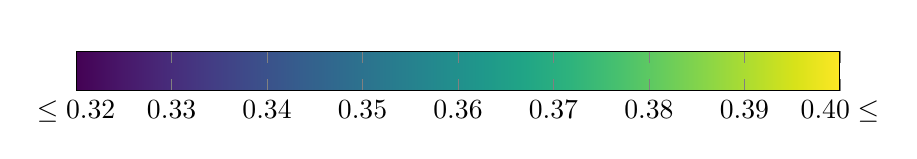
\begin{tikzpicture}
      \begin{axis}[
          hide axis,
          scale only axis,
          height=0pt,
          width=0pt,
          colormap/viridis,
          colorbar horizontal,
          point meta min=0.32,
          point meta max=0.40,
          colorbar style={
              width=0.8\textwidth,
              xtick={0.32, 0.33, 0.34, 0.35, 0.36, 0.37, 0.38, 0.39, 0.40},
              xticklabels={$\le 0.32$, $0.33$, $0.34$, $0.35$, $0.36$, $0.37$, $0.38$, $0.39$, $0.40 \le$}
          }]
          \addplot [draw=none] coordinates {(0,0)};
      \end{axis}
    \end{tikzpicture} \\
    \includegraphics[width=\textwidth]{figures/tube/tube_print_0.png} \\
    \includegraphics[width=\textwidth]{figures/tube/tube_print_1.png} \\
    \includegraphics[width=\textwidth]{figures/tube/tube_print_2.png} \\
    \includegraphics[width=\textwidth]{figures/tube/tube_print_3.png}
  \end{center}
\end{frame}

\section{Making it fast}

\begin{frame}{Layered redundancies}
  \begin{center}
    Algorithmic complexity: $\displaystyle\mathcal{O}(N_t N_s^2)$
  \end{center}
  \vphantom{
    \parbox{\linewidth}{
      \begin{block}{Rotating-wave approximation}
        High-frequency terms barely affect dynamics; formulate equations without them.
      \end{block}
      \begin{block}{Fewer degrees-of-freedom}
        $g(\vb{r}, \vb{r}')$ has the same value at large distances; aggregate sources and transmit once.
      \end{block}
      \begin{block}{Imposed structure}
        $g(\vb{r}, \vb{r}') = \vb{g}(\abs{\vb{r} - \vb{r}'})$; employ FFT to accelerate $\oper{Z}\cdot\oper{A}$.
      \end{block}
      \begin{center}
        Improved algorithmic complexity: $\displaystyle\mathcal{O}\qty(\frac{N_t}{\alpha} N_s \log N_s)$
      \end{center}
    }
  }
\end{frame}

\begin{frame}
  \includegraphics[width=\textwidth, height=0.5cm]{figures/Helium_spectrum_visible}
      \begin{block}{Liouville equation (rotating frame)}
        \begin{gather*}
          \dv{\tilde{\rho}}{t} = -\frac{i}{\hbar} \commutator{\hat{U}\hat{\oper{H}}\hat{U}^\dagger - i\hbar \hat{V}}{\tilde{\rho}} - \hat{\oper{D}}\qty[\tilde{\rho}]; \quad \hat{U} = \mathrm{diag}(1, e^{i \omega_L t}), \quad \hat{V} = \hat{U} \dv{\hat{U}}{t}
        \end{gather*}
      \end{block}

      \begin{gather*}
        \tilde{\mathfrak{F}}\{\tilde{\vb{P}}(\vb{r}, t) \} \equiv -k_2 \int_{}
        \qty(\mathrm{I} -  \outerprod{\bar{\vb{r}}}{\bar{\vb{r}}} ) \cdot \frac{\qty(\partial_t^2 \tilde{\vb{P}}(\vb{r}', t_R) + 2 i \omega_L \partial_t \tilde{\vb{P}}(\vb{r}', t_R) - \omega_L^2 \tilde{\vb{P}}(\vb{r}', t_R)) \alert{e^{-i \omega_L \abs{\vb{r} - \vb{r}'}/c}}}{c^2 \abs{\vb{r}-\vb{r}'}} + \\
        \qty(\mathrm{I} - 3\outerprod{\bar{\vb{r}}}{\bar{\vb{r}}} ) \cdot \frac{\qty(\partial_t \tilde{\vb{P}}(\vb{r}', t_R) + i \omega_L \tilde{\vb{P}}(\vb{r}', t_R))\alert{e^{-i \omega_L \abs{\vb{r} - \vb{r}'}/c}}}{c \abs{\vb{r}-\vb{r}'}^2} +
        \qty(\mathrm{I} - 3\outerprod{\bar{\vb{r}}}{\bar{\vb{r}}} ) \cdot \frac{                \tilde{\vb{P}}(\vb{r}', t_R) \alert{e^{-i \omega_L \abs{\vb{r} - \vb{r}'}/c}}}{\abs{\vb{r}-\vb{r}'}^3}
        \, \dd[3]{\vb{r'}}
      \end{gather*}
\end{frame}

\begin{frame}
  \begin{filecontents}{frames.dat}
0.  1.000000000001855 1.000000000001851
0.0078125 1.000000000099064 1.0000000000019755
0.015625  1.0000000001963325  1.000000000001922
0.0234375 1.0000000002930804  1.000000000001333
0.03125 1.0000000003887002  0.9999999999996733
0.0390625 1.0000000004816654  0.99999999999578
0.046875  1.0000000005701766  0.9999999999868765
0.0546875 1.000000000648538 0.999999999967912
0.0625  1.0000000007038823  0.9999999999284281
0.0703125 1.0000000007228276  0.9999999998480593
0.078125  1.0000000006597871  0.9999999996866216
0.0859375 1.0000000004196619  0.9999999993672697
0.09375 0.999999999913817 0.999999998743509
0.1015625 0.9999999988220319  0.9999999975472348
0.109375  0.9999999965210244  0.9999999952767697
0.1171875 0.999999992495834 0.9999999910144274
0.125 0.999999984749681 0.999999983117343
0.1328125 0.9999999696463988  0.999999968709761
0.140625  0.999999944574401 0.9999999426909157
0.1484375 0.9999998984012756  0.9999998962233709
0.15625 0.9999998122242137  0.9999998142275746
0.1640625 0.9999996745759964  0.9999996716013094
0.171875  0.9999994297548589  0.9999994261139672
0.1796875 0.9999989902485159  0.9999990082085595
0.1875  0.9999983132221766  0.9999983051436087
0.1953125 0.9999971480620461  0.9999971381500145
0.203125  0.9999951345961271  0.9999952222108605
0.2109375 0.9999921417268969  0.9999921112188368
0.21875 0.9999871541975468  0.9999871186923618
0.2265625 0.9999788578642649  0.9999792086530892
0.234375  0.9999669552750505  0.999966816490646
0.2421875 0.9999477381984327  0.9999476168903155
0.25  0.9999169738485708  0.9999182151963328
0.2578125 0.9998743637294126  0.999873741974957
0.265625  0.99980767794116  0.9998072351437279
0.2734375 0.9997049637635869  0.999708882963078
0.28125 0.9995675863746575  0.9995651136235735
0.2890625 0.9993590717629919  0.9993574572954752
0.296875  0.9990501873704873  0.9990609519240244
0.3046875 0.9986511506048743  0.9986423197103002
0.3125  0.9980634868593959  0.9980580611387568
0.3203125 0.9972267476443237  0.997252212373583
0.328125  0.9961824638596517  0.9961535437869212
0.3359375 0.9946899240673321  0.9946727073988877
0.34375 0.992649182213192 0.9927000143584426
0.3515625 0.9901887592838116  0.9901031269954944
0.359375  0.986776789247096 0.9867249236762389
0.3671875 0.9823030803488498  0.9823823547545908
0.375 0.9770950478054405  0.9768676559442772
0.3828125 0.9700944843845721  0.9699505060528694
0.390625  0.9613088848309946  0.961382322341978
0.3984375 0.951444634256464 0.9509035658116819
0.40625 0.9386164534254466  0.9382542473883523
0.4140625 0.9232415015740091  0.9231863590706296
0.421875  0.9066244654085627  0.9054790865778088
0.4296875 0.8857731477146324  0.8849573328595965
0.4375  0.8619532539265771  0.861507853220744
0.4453125 0.8372374076458438  0.8350955940124856
0.453125  0.807399607396371 0.8057775375556345
0.4609375 0.7749346211857239  0.7737150194202129
0.46875 0.7426950502672157  0.7391728479160571
0.4765625 0.7053389437418488  0.7025158862517759
0.484375  0.6665569214321613  0.6641971477031197
0.4921875 0.6298124494607032  0.6247395986046391
0.5 0.588990040104439 0.5847063225831133
0.5078125 0.5483009802567272  0.5446705525378415
0.515625  0.5115743243354371  0.5051830367462833
0.5234375 0.4724042158791771  0.46673629561749463
0.53125 0.43439374240395795 0.4297382500700015
0.5390625 0.401543969323369 0.39449067328032006
0.546875  0.3677568924000411  0.36117830297357223
0.5546875 0.33500332812090355 0.3298625024533398
0.5625  0.30733818378974814 0.3004980187241476
0.5703125 0.2797074923749053  0.2729524850232183
0.578125  0.25206040657657114 0.2470361293078564
0.5859375 0.22838311156005775 0.2225376170178301
0.59375 0.2054225126794082  0.19926468284697763
0.6015625 0.18148787188838852 0.1770807254158882
0.609375  0.1602790821756127  0.1559350345878618
0.6171875 0.14078025239518704 0.135892162867752
0.625 0.12054225557983804 0.1171359322294348
0.6328125 0.10259822385626297 0.09996485644779055
0.64  0.08810711896012689 0.08590234347027573
0.640078125 0.08814108013224162 0.08575994015812884
0.64015625  0.08820740455562986 0.08561777604236251
0.640234375 0.08827897706626837 0.08547585158440088
0.6403125 0.088328087682513 0.0853341672456689
0.640390625 0.08832993955631298 0.08519272348759069
0.64046875  0.0882657843872815  0.08505152077159096
0.640546875 0.08812528842769907 0.08491055955909446
0.640625  0.08790782690598993 0.08476984031152532
0.640625  0.08790782690598993 0.08476984031152532
0.640703125 0.08762255053414066 0.08462936349030827
0.64078125  0.08728721438033753 0.08448912955686802
0.640859375 0.08692591578047199 0.08434913897262872
0.6409375 0.08656603615500583 0.0842093921990151
0.641015625 0.08623476900186558 0.08406988969745187
0.64109375  0.08595567704531715 0.08393063192936318
0.641171875 0.0857457157484245  0.08379161935617395
0.64125 0.0856130926867289  0.08365285243930831
0.641328125 0.08555624377941436 0.083514331640191
0.64140625  0.08556404548384543 0.08337605742024673
0.641484375 0.08561723470782384 0.08323803024089965
0.6415625 0.08569086192458497 0.08310025056357448
0.641640625 0.08575745751699647 0.08296271884969593
0.64171875  0.08579051322370179 0.08282543556068817
0.641796875 0.08576783788264283 0.0826884011579759
0.641875  0.08567435938716023 0.08255161610298387
0.641953125 0.08550402384489701 0.08241508085713618
0.64203125  0.08526054974172712 0.0822787958818576
0.642109375 0.08495694122551838 0.08214276163857283
0.6421875 0.08461382976013858 0.082006978588706
0.642265625 0.08425685108265485 0.08187144719368204
0.64234375  0.08391339089112217 0.0817361679149251
0.642421875 0.08360911628330307 0.0816011412138599
0.6425  0.08336472618833213 0.08146636755191115
0.642578125 0.08319333903767537 0.08133184739050302
0.64265625  0.08309884364013581 0.0811975811910602
0.642734375 0.08307541683797595 0.08106356941500743
0.6428125 0.08310827858528745 0.08092981252376885
0.642890625 0.0831755758934856  0.08079631097876919
0.64296875  0.0832511592262399  0.08066306524143316
0.643046875 0.08330790171617586 0.08053007577318491
0.643125  0.08332113421617802 0.08039734303544936
0.643203125 0.08327176632738928 0.08026486748965064
0.64328125  0.08314869575005751 0.0801326495972135
0.643359375 0.08295020088022002 0.08000068981956263
0.6434375 0.0826841467591189  0.0798689886181222
0.643515625 0.08236697521888331 0.07973754645431691
0.64359375  0.08202160898574397 0.0796063637895715
0.643671875 0.08167454095406408 0.0794754410853101
0.64375 0.08135247326063887 0.07934477880295746
0.643828125 0.08107893562021959 0.07921437740393826
0.64390625  0.08087131138755854 0.07908423734967668
0.643984375 0.0807386424408842  0.07895435910159743
0.6440625 0.08068049917743224 0.07882474312112521
0.644140625 0.08068704906777732 0.0786953898696842
0.64421875  0.08074031322574558 0.07856629980869931
0.644296875 0.08081645858623532 0.07843747339959466
0.644375  0.08088882347043677 0.078308911103795
0.644453125 0.08093129844440325 0.07818061338272503
0.64453125  0.0809216326115854  0.0780525806978089
0.644609375 0.08084424424813852 0.07792481351047136
0.6446875 0.0806921859364035  0.07779731228213707
0.644765625 0.08046801112432066 0.07767007747423024
0.64484375  0.08018343544178011 0.07754310954817556
0.644921875 0.07985784117000153 0.07741640896539774
0.645 0.07951581066995092 0.07728997618732096
0.645078125 0.07918400482890496 0.0771638116753701
0.64515625  0.07888778444737768 0.07703791589096935
0.645234375 0.07864799858885671 0.07691228929554339
0.6453125 0.07847835202157986 0.07678693235051694
0.645390625 0.0783836806343218  0.07666184551731418
0.64546875  0.07835934949746455 0.07653703223473818
0.645546875 0.0783918574388659  0.07641250644045161
0.645625  0.07846055964083352 0.07628825212136112
0.645703125 0.07854029201556798 0.07616426972076673
0.64578125  0.07860456727594056 0.07604055968196852
0.645859375 0.07862893003818357 0.07591712244826598
0.6459375 0.07859405267040945 0.07579395846295918
0.646015625 0.07848817500888901 0.07567106816934817
0.64609375  0.07830858128410229 0.07554845201073246
0.646171875 0.07806193269485938 0.0754261104304123
0.64625 0.0777634086540806  0.07530404387168718
0.646328125 0.07743477073187746 0.07518225277785719
0.64640625  0.07710159774820448 0.07506073759222234
0.646484375 0.07679003905267649 0.0749394987580822
0.6465625 0.07652350177906327 0.07481853671873678
0.646640625 0.07631969044488397 0.07469785191748614
0.64671875  0.07618837101421562 0.07457744479762982
0.646796875 0.07613014809759341 0.07445731580246785
0.646875  0.07613640207098007 0.0743374653753003
0.646953125 0.07619039298212005 0.07421789395942667
0.64703125  0.07626939642454834 0.0740986019981472
0.647109375 0.07634758980697254 0.07397958993476142
0.6471875 0.07639932858000073 0.07386085821256938
0.647265625 0.0764023949181377  0.07374240727487111
0.64734375  0.07634080543909538 0.07362423756496615
0.647421875 0.07620682880906347 0.07350634952615456
0.6475  0.07600195112478404 0.07338874360173636
0.647578125 0.07573667305519621 0.07327142023501111
0.64765625  0.07542916797738253 0.07315437986927883
0.647734375 0.07510296685228852 0.07303762294783958
0.6478125 0.07478396919375077 0.0729211499139929
0.647890625 0.0744971590122656  0.07280496121103883
0.64796875  0.07426343979545755 0.0726890572822774
0.648046875 0.07409699373305043 0.07257343857100815
0.648125  0.07400349500568426 0.07245810552053131
0.648203125 0.07397940226677097 0.07234305857414641
0.64828125  0.07401242405527123 0.07222829817515349
0.648359375 0.07408308862853392 0.07211382476685259
0.6484375 0.07416722115440885 0.07199963879254326
0.6484375 0.07416722115440885 0.07199963879254326
0.648515625 0.07423901562321328 0.07188574069552553
0.64859375  0.07427430507721927 0.07177213091909944
0.648671875 0.0742536228526816  0.07165880990656455
0.64875 0.07416466052782565 0.07154577810122088
0.648828125 0.07400381548959395 0.07143303594636849
0.64890625  0.073776636746983 0.07132058388530692
0.648984375 0.07349710592468317 0.07120842236133636
0.6490625 0.07318585298314453 0.07109655181775636
0.649140625 0.07286753349800455 0.07098497269786697
0.64921875  0.07256769725175928 0.07087368544496822
0.649296875 0.07230955026261175 0.07076269050235967
0.649375  0.07211101774993015 0.07065198831334134
0.649453125 0.07198247981638828 0.07054157932121327
0.64953125  0.07192546961230217 0.07043146396927503
0.649609375 0.07193249193680298 0.07032164270082664
0.6496875 0.07198798592675404 0.07021211595916813
0.649765625 0.07207031159474599 0.07010288418759908
0.64984375  0.0721545000378863  0.06999394782941949
0.649921875 0.07221542311829683 0.06988530732792941
0.65  0.07223097815798733 0.06977696312642842
0.650078125 0.07218488250664157 0.06966891566821667
0.65015625  0.07206873081468022 0.06956116539659375
0.650234375 0.07188304566104599 0.06945371275485968
0.6503125 0.07163719756554845 0.0693465581863145
0.650390625 0.07134820625411407 0.06923970213425774
0.65046875  0.07103857013368038 0.06913314504198949
0.650546875 0.07073340744909123 0.06902688735280972
0.650625  0.07045726932496857 0.06892092951001803
0.650703125 0.07023102829958552 0.06881527195691445
0.65078125  0.0700692399937986  0.06870991513679899
0.650859375 0.06997830724006503 0.06860485949297122
0.6509375 0.06995568056897085 0.06850010546873134
0.651015625 0.06999019714120225 0.0683956535073789
0.65109375  0.07006350772833699 0.06829150405221396
0.651171875 0.07015241327962812 0.0681876575465365
0.65125 0.07023181398024571 0.0680841144336461
0.651328125 0.0702778918911127  0.06798087515684283
0.65140625  0.07027112946025262 0.06787794015942666
0.651484375 0.0701987753030866  0.0677753098846972
0.6515625 0.07005644903638406 0.06767298477595447
0.651640625 0.06984868678724282 0.06757096527649847
0.65171875  0.06958834967009737 0.06746925182962882
0.651796875 0.06929498165972357 0.06736789543045793
0.651875  0.06899232343674756 0.06726684908832516
0.651953125 0.0687052952450832  0.0671661100314298
0.65203125  0.06845683745381864 0.06706567865297201
0.652109375 0.06826500497740279 0.06696555534615134
0.6521875 0.06814068582370984 0.0668657405041678
0.652265625 0.06808623346033273 0.06676623452022136
0.65234375  0.06809518034754494 0.06666703778751161
0.652421875 0.06815307139932492 0.06656815069923852
0.6525  0.06823931027264164 0.0664695736486021
0.652578125 0.06832977852438309 0.06637130702880191
0.65265625  0.0683998991611126  0.06627335123303794
0.652734375 0.06842775289029021 0.0661757066545102
0.6528125 0.06839685147692595 0.06607837368641822
0.652890625 0.06829822215735327 0.06598135272196216
0.65296875  0.06813153117495734 0.06588464415434159
0.653046875 0.06790511290327368 0.0657882483767565
0.653125  0.06763490265604469 0.06569216578240686
0.653203125 0.06734240221335941 0.06559639676449228
0.65328125  0.06705194671293012 0.06550094171621271
0.653359375 0.06678761509429794 0.06540580103076815
0.6534375 0.06657017702975157 0.06531097510135819
0.653515625 0.0664144660139083  0.06521646432118282
0.65359375  0.06632750624855682 0.065122269083442
0.653671875 0.06630763439276209 0.06502838978133534
0.65375 0.06634472515877095 0.0649348268080628
0.653828125 0.06642148671243726 0.06484158055682437
0.65390625  0.06651566468462637 0.06474865142081965
0.653984375 0.06660287216060744 0.06465603979324873
0.6540625 0.06665968397842269 0.06456374606731122
0.654140625 0.06666660681081031 0.0644717706362071
0.65421875  0.06661054360169429 0.06438011389313633
0.654296875 0.06648644391635915 0.06428877623129853
0.654375  0.06629793484732202 0.06419775804389366
0.654453125 0.06605684508229143 0.0641070597241217
0.65453125  0.06578169352102156 0.06401668166518225
0.654609375 0.0654953322715458  0.06392662426027529
0.6546875 0.06522204052383124 0.06383688790260078
0.654765625 0.06498444510746813 0.06374747298535835
0.65484375  0.06480065239077341 0.06365837990174808
0.654921875 0.06468195934600758 0.06356960904496957
0.655 0.06463143243530757 0.0634811608082228
0.655078125 0.0646435294051861  0.06339303558470774
0.65515625  0.06470481616783372 0.06330523376762401
0.655234375 0.06479568334493462 0.06321775575017155
0.6553125 0.06489284133869494 0.06313060192555037
0.655390625 0.06497228043544613 0.06304377268696006
0.65546875  0.06501231649996626 0.06295726842760059
0.655546875 0.06499633690440566 0.06287108954067194
0.655625  0.06491490152022052 0.06278523641937371
0.655703125 0.0647669271689718  0.06269970945690587
0.65578125  0.06455981273867285 0.0626145090464684
0.655859375 0.06430849033740865 0.0625296355812609
0.6559375 0.06403351763225325 0.06244508945448348
0.656015625 0.06375846358488597 0.06236087105933573
0.65609375  0.06350691435869253 0.062276980789017625
0.656171875 0.06329948118200093 0.06219341903672914
0.65625 0.06315119179722412 0.06211018619566988
0.65625 0.06315119179722412 0.06211018619566988
0.656328125 0.06306959053352984 0.062027282659039826
0.65640625  0.06305379380492306 0.061944708820038934
0.656484375 0.06309461557870902 0.06186246507186683
0.6565625 0.06317574335306572 0.061780551807723474
0.656640625 0.06327581925301778 0.06169896942080884
0.65671875  0.06337115688327749 0.061617718304322534
0.656796875 0.06343874874064366 0.06153679885146465
0.656875  0.06345918480114096 0.06145621145543481
0.656953125 0.06341910817266055 0.06137595650943297
0.65703125  0.06331290060313956 0.061296034406659095
0.657109375 0.06314338552108156 0.06121644554031282
0.6571875 0.06292145521958731 0.06113719030359409
0.657265625 0.06266467824727003 0.06105826908970288
0.65734375  0.06239506196449207 0.06097968229183882
0.657421875 0.06213625247489198 0.060901430303201866
0.6575  0.06191053400465184 0.06082351351699198
0.657578125 0.06173600201700682 0.06074593232640879
0.65765625  0.06162427447254098 0.06066868712465226
0.657734375 0.06157902817894703 0.06059177830492235
0.6578125 0.06159554158986679 0.06051520626041869
0.657890625 0.06166130799486874 0.06043897138434135
0.65796875  0.06175763390702269 0.06036307406988996
0.658046875 0.061862018787504844  0.06028757584560126
0.658125  0.06195101661513764 0.0602124386425244
0.658203125 0.06200321141210541 0.060137640045443044
0.65828125  0.06200193158574122 0.06006318036934351
0.658359375 0.0619373594250424  0.059989059929212114
0.6584375 0.061807765256678686  0.059915279040034866
0.658515625 0.061619716089415175  0.0598418380167981
0.65859375  0.06138723175212602 0.05976873717448813
0.658671875 0.06112999338072957 0.059695976828090955
0.65875 0.06087083938772382 0.05962355729259302
0.658828125 0.06063286253375529 0.05955147888298032
0.65890625  0.06043647882291566 0.05947974191423917
0.658984375 0.060296841900937835  0.05940834670135591
0.6590625 0.06022192485323164 0.059337293559316544
0.659140625 0.06021152069367314 0.05926658280310739
0.65921875  0.06025728050114216 0.05919621474771476
0.659296875 0.06034378259839797 0.05912618970812468
0.659375  0.060450501633719705  0.059056507999323465
0.659453125 0.060554420179853664  0.05898716993629743
0.65953125  0.06063295308233593 0.058918175834032596
0.659609375 0.06066681397779414 0.05884952600751527
0.6596875 0.06064245711329003 0.058781220771731785
0.659765625 0.060553789182434016  0.05871326044166815
0.65984375  0.06040293305640231 0.05864564533231078
0.659921875 0.0601999452874749  0.0585783757586457
0.66  0.05996153002298003 0.05851145203565921
0.660078125 0.05970891017553081 0.05844487447833765
0.66015625  0.059465126387464075  0.05837864340166703
0.660234375 0.05925211148797754 0.058312759120633655
0.6603125 0.05908790640039823 0.05824722195022385
0.660390625 0.058984376598680895  0.058182032205423645
0.66046875  0.05894571523791116 0.05811719020121934
0.660546875 0.05896791858432998 0.058052696252597256
0.660625  0.05903930816605973 0.05798855067454342
0.660703125 0.05914202326510009 0.05792475378204423
0.66078125  0.05925429551667054 0.05786130589008573
0.660859375 0.05935321894816722 0.05779820731365422
0.6609375 0.05941765820851877 0.057735458367736005
0.661015625 0.05943092970103981 0.057673059367317134
0.66109375  0.059382913803351284  0.057611010627383906
0.661171875 0.0592713293332474  0.05754931246292263
0.66125 0.059102013966473806  0.05748796518891935
0.661328125 0.05888817271483653 0.057426969120360355
0.66140625  0.058648690538352435  0.057366324572231966
0.661484375 0.058405728678881115  0.057306031859520226
0.6615625 0.05818190630589151 0.05724609129721143
0.661640625 0.057997428137140816  0.05718650320029189
0.66171875  0.05786752347206813 0.05712726788374764
0.661796875 0.057800516628577804  0.05706838566256508
0.661875  0.05779678132407209 0.05700985685173025
0.661953125 0.057848703673508584  0.056951681766229466
0.66203125  0.057941657111501975  0.05689386072104901
0.662109375 0.05805587122254006 0.056836394031174936
0.6621875 0.05816894764648636 0.05677928201159356
0.662265625 0.05825870744730225 0.05672252497729116
0.66234375  0.05830600755162276 0.056666123243253805
0.662421875 0.05829716625624721 0.05661007712446779
0.6625  0.05822569479862231 0.05655438693591941
0.662578125 0.058093111982682896  0.05649905299259472
0.66265625  0.05790874006941133 0.05644407560948011
0.662734375 0.05768851270885682 0.05638945510156162
0.6628125 0.05745294315345653 0.05633519178382556
0.662890625 0.05722451310320259 0.05628128597125822
0.66296875  0.05702481639453347 0.05622773797884566
0.663046875 0.05687181651329287 0.05617454812157418
0.663125  0.056777570867026915  0.05612171671443007
0.663203125 0.05674670738435166 0.056069244072399396
0.66328125  0.05677584335738952 0.05601713051046846
0.663359375 0.05685402773932955 0.05596537634362353
0.6634375 0.05696414054351219 0.0559139818868507
0.663515625 0.05708507355954645 0.05586294745513625
0.66359375  0.05719441771208172 0.05581227336346647
0.663671875 0.057271309277280844  0.055761959926827434
0.66375 0.05729907883630142 0.05571200746020551
0.663828125 0.057267363008492035  0.05566241627858675
0.66390625  0.05717341200835664 0.055613186696957466
0.663984375 0.05702243158267338 0.05556431903030394
0.6640625 0.05682691184781345 0.05551581359361225
0.6640625 0.05682691184781345 0.05551581359361225
0.664140625 0.05660503171073579 0.05546767070186867
0.66421875  0.05637834449983053 0.0554198906700595
0.664296875 0.05616903565673643 0.055372529215186435
0.664375  0.055997104284671695  0.055325582982748464
0.664453125 0.05587782587173819 0.05527900040357609
0.66453125  0.055819815605573114  0.05523278169269518
0.664609375 0.055823943576816 0.055186927065131834
0.6646875 0.05588323304545358 0.05514143673591191
0.664765625 0.0559837537058872  0.055096310920061446
0.66484375  0.05610640181495475 0.05505154983260648
0.664921875 0.056229331566222895  0.05500715368857288
0.665 0.056330733549222085  0.05496312270298669
0.665078125 0.05639160562438954 0.054919457090873945
0.66515625  0.05639816236235884 0.0548761570672605
0.665234375 0.05634358231404482 0.054833222847172396
0.6653125 0.05622886582997582 0.054790654645635685
0.665390625 0.05606269876210981 0.05474845267767622
0.66546875  0.05586034236070288 0.05470661715832004
0.665546875 0.05564168647003848 0.054665148302593176
0.665625  0.05542871765718874 0.05462404632552151
0.665703125 0.05524272433218179 0.05458331144213113
0.66578125  0.055101591734310985  0.0545429438674479
0.665859375 0.05501753424366715 0.05450294381649786
0.6659375 0.05499554943110425 0.05446331150430704
0.666015625 0.05503278904905412 0.05442404714590132
0.66609375  0.055118931453641974  0.05438515095630673
0.666171875 0.05523750017016062 0.0543466231505493
0.66625 0.055367962923988184  0.05430846394365491
0.666328125 0.05548834633061735 0.054270673550649594
0.66640625  0.05557802777313756 0.05423325218655938
0.666484375 0.05562035582757459 0.05419620006641015
0.6665625 0.055604761060289644  0.05415951740522798
0.666640625 0.05552809199321641 0.05412320441803875
0.66671875  0.05539501028981515 0.0540872613198685
0.666796875 0.05521738917445242 0.054051688325743245
0.666875  0.055012797595185584  0.05401648565068888
0.666953125 0.05480226335952101 0.053981653509731435
0.66703125  0.05460759674439812 0.053947192117896926
0.667109375 0.05444861880433486 0.05391310169021125
0.6671875 0.05434064444736565 0.05387938244170043
0.667265625 0.05429253945343874 0.05384603458739049
0.66734375  0.05430560155237896 0.053813058342307325
0.667421875 0.05437340210327998 0.053780453921476956
0.6675  0.0544826092889188  0.053748221539925416
0.667578125 0.0546146909073177  0.05371636141267858
0.66765625  0.054748273223192305  0.05368487375476253
0.667734375 0.05486186030931973 0.05365375878120316
0.6678125 0.05493656623998307 0.05362301670702649
0.667890625 0.0549585114742147  0.05359264774725854
0.66796875  0.054920584584085726  0.05356265211692521
0.668046875 0.05482333805367139 0.053533030031052524
0.668125  0.05467491108510307 0.05350378170466649
0.668203125 0.05448999042186758 0.05347490735279303
0.66828125  0.05428793651696975 0.05344640719045815
0.668359375 0.05409031939935218 0.05341828143268787
0.6684375 0.05391817560971195 0.0533905302945081
0.668515625 0.05378933407194843 0.053363153990944885
0.66859375  0.053716153782714396  0.053336152737024134
0.668671875 0.053703956865006335  0.053309526747771875
0.66875 0.053750357236090174  0.05328327623821412
0.668828125 0.05384557208455499 0.05325740142337677
0.66890625  0.05397367052878838 0.05323190251828584
0.668984375 0.054114603369124506  0.053206779737967363
0.6690625 0.054246756077184655  0.05318203329744724
0.669140625 0.05434969610277104 0.053157663411751474
0.66921875  0.05440677066474427 0.0531336702959061
0.669296875 0.054407219299299085  0.05311005416493701
0.669375  0.054347536217319053  0.05308681523387024
0.669453125 0.05423191291655616 0.05306395371773179
0.66953125  0.05407169714392436 0.05304146983154757
0.669609375 0.05388394556059359 0.05301936379034364
0.6696875 0.05368925240903529 0.052997635809145904
0.669765625 0.05350912775481609 0.05297628610298038
0.66984375  0.053363263369406486  0.05295531488687308
0.669921875 0.053267030210645404  0.052934722375849924
0.67  0.053229527082951235  0.05291450878493692
0.670078125 0.0532524297655755  0.05289467432916007
0.67015625  0.053329782201164355  0.052875219223545315
0.670234375 0.0534487588777664  0.05285614368311865
0.6703125 0.05359130158812412 0.05283744792290609
0.670390625 0.053736417708587905  0.05281913215793355
0.67046875  0.0538628515928262  0.05280119660322708
0.670546875 0.05395178699017423 0.05278367868391237
0.670625  0.05398923632928322 0.05276662624627358
0.670703125 0.05396781809747505 0.052749954515420354
0.67078125  0.05388768869572703 0.05273366359252092
0.670859375 0.05375651773814722 0.05271775357874357
0.6709375 0.053588510391647706  0.0527022245752566
0.671015625 0.053402595141347875  0.05268707668322822
0.67109375  0.05322001544129964 0.052672310003826744
0.671171875 0.05306162745952843 0.052657924638220444
0.67125 0.05294524804658106 0.05264392068757756
0.671328125 0.05288339238916874 0.052630298253066386
0.67140625  0.05288168466698189 0.052617057435855194
0.671484375 0.052938147127645524  0.05260419833711224
0.6715625 0.05304345722105608 0.05259172105800581
0.671640625 0.053182135973596174  0.05257962569970415
0.67171875  0.05333451994705697 0.05256791236337553
0.671796875 0.053479264402815946  0.05255658115018827
0.671875  0.053596057140996245  0.05254563216131058
0.671875  0.053596057140996245  0.05254563216131058
0.671953125 0.05366820182865582 0.05253506549791075
0.67203125  0.053684737803655284  0.05252488126115708
0.672109375 0.053641830029818593  0.05251507955221779
0.6721875 0.05354325556404356 0.052505660472261184
0.672265625 0.05339991679810188 0.05249662412245553
0.67234375  0.05322845253376252 0.05248797060396908
0.672421875 0.05304912067663186 0.05247970001797013
0.6725  0.052883219193602816  0.05247181246562692
0.672578125 0.05275037877117718 0.052464308048107734
0.67265625  0.05266606636258341 0.05245718686658086
0.672734375 0.052639620554941494  0.05245044902221453
0.6728125 0.05267306791713632 0.052444094616177044
0.672890625 0.05276086703115364 0.052438123749636675
0.67296875  0.052890617133887666  0.05243253652376167
0.673046875 0.053044638824040174  0.05242733303972031
0.673125  0.05320222341153903 0.05242251339868087
0.673203125 0.0533422682825256  0.052418077701811616
0.67328125  0.053445960153726726  0.05241402605028082
0.673359375 0.05349916578249165 0.05241035854525675
0.6734375 0.05349422894129572 0.05240707528790767
0.673515625 0.05343093956507867 0.05240417637940186
0.67359375  0.05331655780507775 0.05240166192090759
0.673671875 0.05316489017182321 0.05239953201359312
0.67375 0.05299452920052582 0.05239778675862673
0.673828125 0.05282648890715073 0.052396426257176686
0.67390625  0.05268153150992295 0.05239545061041126
0.673984375 0.05257752688042467 0.05239485991949872
0.6740625 0.0525271821795235  0.05239465428560734
0.674140625 0.05253642573149452 0.05239483380990539
0.67421875  0.052603656197067424  0.052395398593561134
0.674296875 0.05271994925324703 0.05239634873774284
0.674375  0.05287019325247082 0.052397684343618786
0.674453125 0.053035013729877296  0.05239940551235724
0.67453125  0.05319323858007412 0.05240151234512648
0.674609375 0.05332459031524763 0.05240400494309476
0.6746875 0.053412265447394365  0.052406883407430355
0.674765625 0.05344506926754515 0.05241014783930154
0.67484375  0.053418837983677595  0.05241379833987658
0.674921875 0.0533369682010393  0.05241783501032376
0.675 0.05320998111603933 0.05242225795181134
0.675078125 0.05305418387401389 0.05242706726550757
0.67515625  0.05288959561572  0.05243226305258075
0.675234375 0.05273739943975437 0.052437845414199144
0.6753125 0.052617249810284185  0.052443814451531
0.675390625 0.052544771811885806  0.05245017026574462
0.67546875  0.0525295755579817  0.052456912958008244
0.675546875 0.05257403584398542 0.05246404262949017
0.675625  0.052672989302112075  0.052471559381358654
0.675703125 0.052814393727253335  0.05247946331478196
0.67578125  0.052980860801578177  0.052487754530928375
0.675859375 0.05315186721944054 0.05249643313096616
0.6759375 0.05330636609242617 0.05250549921606357
0.676015625 0.05342546295147372 0.0525149528873889
0.67609375  0.053494818199528164  0.052524794246110416
0.676171875 0.05350647115671658 0.052535023393396364
0.67625 0.05345985011150632 0.05254564043041505
0.676328125 0.05336184495239859 0.0525566454583347
0.67640625  0.053225931637344716  0.052568038578323636
0.676484375 0.05307045619215959 0.052579819891550104
0.6765625 0.05291630267321628 0.05259198949918235
0.676640625 0.052784236798591976  0.05260454750238868
0.67671875  0.05269226491445671 0.05261749400233736
0.676796875 0.05265334538004773 0.05263084098833951
0.676875  0.05267373838524919 0.05264469304721515
0.676953125 0.05275221174858598 0.05265893377561693
0.67703125  0.05288019798056963 0.05267356315507839
0.677109375 0.05304288223739702 0.05268858116713311
0.6771875 0.053221087966358084  0.052703987793314644
0.677265625 0.05339371521005323 0.05271978301515651
0.67734375  0.053540423563488745  0.0527359668141923
0.677421875 0.05364421959211331 0.05275253917195552
0.6775  0.053693616749063026  0.05276950006997977
0.677578125 0.053684096818793846  0.05278684948979858
0.67765625  0.05361868561254975 0.05280458741294547
0.677734375 0.053507566961917004  0.052822713820954055
0.6778125 0.053366789267172844  0.052841228695357845
0.677890625 0.05321622559399106 0.052860132017690374
0.67796875  0.053077045773452736  0.05287942376948525
0.678046875 0.05296902579864751 0.05289910393227599
0.678125  0.05290803109262367 0.05291917248759612
0.678203125 0.052903999606372216  0.05293962941697924
0.67828125  0.05295967794625774 0.05296047470195886
0.678359375 0.053070268680805874  0.05298170832406857
0.6784375 0.053224041746264404  0.053003330264841914
0.678515625 0.05340382480590419 0.053025340505812396
0.67859375  0.05358918528019979 0.05304773902851364
0.678671875 0.053759029363404334  0.05307052581447916
0.67875 0.053894283327145034  0.053093700845242474
0.678828125 0.05398031973530614 0.0531172641023372
0.67890625  0.054008818594251905  0.053141215567296854
0.678984375 0.05397882508944606 0.05316555522165496
0.6790625 0.053896873504469624  0.05319028304694514
0.679140625 0.053776158288800315  0.0532153990247009
0.67921875  0.053634856474161025  0.053240903136455756
0.679296875 0.05349381870333758 0.05326679536374334
0.679375  0.05337391799373811 0.05329307568809713
0.679453125 0.05329339553819971 0.05331974409105074
0.67953125  0.05326554159270441 0.0533468005541377
0.679609375 0.053297001675734264  0.05337424505889151
0.6796875 0.053386931992530716  0.0534020775868458
0.6796875 0.053386931992530716  0.0534020775868458
0.679765625 0.05352710462636057 0.05343029811953409
0.67984375  0.05370294977037782 0.053458906638489886
0.679921875 0.05389540877338757 0.05348790312524682
0.68  0.05408335530519383 0.05351728756133841
0.680078125 0.05424628103043752 0.053547059928298155
0.68015625  0.05436690394102859 0.05357722020765969
0.680234375 0.05443336551431159 0.053607768380956496
0.6803125 0.054440741335039414  0.05363870442972219
0.680390625 0.05439166942864437 0.0536700283354903
0.68046875  0.05429601623587821 0.053701740079794315
0.680546875 0.05416962601010019 0.05373383964416789
0.680625  0.05403230834126502 0.05376632701014452
0.680703125 0.05390532040622395 0.05379920215925772
0.68078125  0.05380866582820875 0.05383246507304113
0.680859375 0.05375854942955377 0.053866115733028255
0.6809375 0.053765316417695275  0.053900154120752594
0.681015625 0.05383213523383991 0.0539345802177478
0.68109375  0.053954589132603814  0.05396939400554738
0.681171875 0.054121237365424575  0.054004595465684826
0.68125 0.054315066060604766  0.05404018457969379
0.681328125 0.054515648060584045  0.05407616132910773
0.68140625  0.054701739952576565  0.054112525695460295
0.681484375 0.05485398121361293 0.05414927766028498
0.6815625 0.05495735735711809 0.05418641720511529
0.681640625 0.0550031104005989  0.05422394431148489
0.68171875  0.05498985399951346 0.054261858960927264
0.681796875 0.05492375469217327 0.05430016113497591
0.681875  0.05481775114982532 0.0543388508151645
0.681953125 0.05468991198103426 0.05437792798302652
0.68203125  0.0545611425095169  0.05441739262009547
0.682109375 0.054452527924774355  0.054457244707905014
0.6821875 0.05438265319691373 0.054497484227988585
0.682265625 0.05436523969651705 0.05453811116187985
0.68234375  0.054407396387794224  0.05457912549111231
0.682421875 0.05450871443132233 0.05462052719721945
0.6825  0.05466131494589671 0.05466231626173494
0.682578125 0.05485084445135392 0.054704492666192275
0.68265625  0.05505829841923942 0.054747056392124946
0.682734375 0.055262433165399936  0.05479000742106663
0.6828125 0.05544246527426892 0.0548333457345508
0.682890625 0.0555807139748245  0.054877071314110966
0.68296875  0.055664849051136445  0.0549211841412808
0.683046875 0.05568946291991004 0.054965684197593775
0.683125  0.05565676112914973 0.05501068301457238
0.683203125 0.05557628591284415 0.05505608405184906
0.68328125  0.05546370941210232 0.05510187204068137
0.683359375 0.055338844797502874  0.05514804684445322
0.6834375 0.05522313056958169 0.055194608326548315
0.683515625 0.05513690743546578 0.05524155635035036
0.68359375  0.055096831147170754  0.05528889077924324
0.683671875 0.05511375418525358 0.05533661147661066
0.68375 0.05519134251612104 0.05538471830583633
0.683828125 0.05532560302344418 0.05543321113030414
0.68390625  0.05550538813113239 0.055482089813397785
0.683984375 0.05571380699900308 0.05553135421850098
0.6840625 0.055930367423216464  0.055581004208997614
0.684140625 0.05613357928337414 0.05563103964827132
0.68421875  0.05630368343710382 0.055681460399706006
0.684296875 0.05642516545945917 0.05573226632668536
0.684375  0.05648872931864892 0.0557834572925931
0.684453125 0.056492482244531544  0.055835033160813105
0.68453125  0.05644218260200674 0.0558869937947291
0.684609375 0.05635051239962431 0.055939339057724746
0.6846875 0.05623547074503349 0.055992068813183984
0.684765625 0.056118091745411894  0.0560451829244905
0.68484375  0.05601977303875805 0.056098681255027975
0.684921875 0.05595955760857611 0.05615256366818033
0.685 0.05595171214026582 0.056206830027331275
0.685078125 0.056003909176236814  0.05626148019586447
0.68515625  0.056116248608505837  0.05631651403716386
0.685234375 0.05628123841356586 0.05637193141461304
0.6853125 0.056484739363887065  0.05642773219159594
0.685390625 0.05670775834534491 0.05648391623149625
0.68546875  0.05692885650915942 0.056540483397697655
0.685546875 0.057126871762436165  0.05659743355358408
0.685625  0.05728360787847496 0.056654766562539205
0.685703125 0.0573861474456664  0.05671248228794673
0.68578125  0.057428499611186005  0.05677058059319058
0.685859375 0.05741236512226799 0.056829061341654434
0.6859375 0.057346926464397985  0.05688792439672198
0.686015625 0.05724768943463807 0.05694716962177715
0.68609375  0.05713451728064613 0.05700679688020354
0.686171875 0.057029111506164416  0.05706680603538509
0.68625 0.056952256861220005  0.05712719695070548
0.686328125 0.05692117918750957 0.05718796948954839
0.68640625  0.056947354994216035  0.05724912351529776
0.686484375 0.057035047732598314  0.057310658891337275
0.6865625 0.057180758737708594  0.057372575481050604
0.686640625 0.05737366648338269 0.0574348731478217
0.68671875  0.0575969936520282  0.05749755175503423
0.686796875 0.05783013258476451 0.057560611166071876
0.686875  0.058051260695413914  0.05762405124431859
0.686953125 0.05824010985643852 0.05768787185315804
0.68703125  0.05838054399483016 0.05775207285597391
0.687109375 0.05846261110239163 0.05781665411615014
0.6871875 0.05848381228365139 0.05788161549707032
0.687265625 0.05844942863123504 0.0579469568621184
0.68734375  0.058371855606632606  0.05801267807467805
0.687421875 0.05826903599349113 0.05807877899813294
0.6875  0.058162187490099465  0.05814525949586704
0.6875  0.058162187490099465  0.05814525949586704
0.687578125 0.058073110004902714  0.05821211943126401
0.68765625  0.058021418471719 0.058279358667707525
0.687734375 0.05802204900866198 0.05834697706858154
0.6878125 0.058083356790927104  0.05841497449726972
0.687890625 0.05820604974439511 0.05848335081715575
0.68796875  0.058383089916971054  0.05855210589162359
0.688046875 0.05860057908701757 0.05862123958405679
0.688125  0.058839518347862184  0.05869075175783933
0.688203125 0.05907821447713426 0.058760642276354885
0.68828125  0.059295032585520456  0.0588309110029871
0.688359375 0.05947114343357251 0.05890155780111996
0.6884375 0.05959291591533275 0.05897258253413713
0.688515625 0.059653655773104684  0.059043985065422265
0.68859375  0.059654460266503916  0.05911576525835934
0.688671875 0.05960408701851977 0.059187922976332026
0.68875 0.05951785214930684 0.059260458082723975
0.688828125 0.059415690444517257  0.059333370440919166
0.68890625  0.059319630226157403  0.05940665991430127
0.688984375 0.059250998783417726  0.05948032636625393
0.6890625 0.05922771320145153 0.05955436966016114
0.689140625 0.05926200300502098 0.05962878965940644
0.68921875  0.05935885006862658 0.059703586227373824
0.689296875 0.059515348146524205  0.059778759227446944
0.689375  0.05972106456460329 0.05985438813485205
0.689453125 0.05995935524615899 0.059930432614869376
0.68953125  0.060209471143817694  0.060006852931824534
0.689609375 0.06044918853469796 0.06008364883802902
0.6896875 0.06065762748128572 0.060160820085794674
0.689765625 0.06081790525333238 0.06023836642743301
0.68984375  0.060919282552774665  0.060316287615255516
0.689921875 0.0609585327495841  0.06039458340157404
0.69  0.06094036261344605 0.06047325353869997
0.690078125 0.06087682087960525 0.060552297778945156
0.69015625  0.06078577815848654 0.060631715874621094
0.690234375 0.060688666415328545  0.06071150757803928
0.6903125 0.06060776139754951 0.060791672641511564
0.690390625 0.06056335758225517 0.06087221081734945
0.69046875  0.06057118901485225 0.06095312185786444
0.690546875 0.060640427125383735  0.06103440551536837
0.690625  0.06077251016033745 0.061116061542172744
0.690703125 0.060960950025547654  0.06119808969058907
0.69078125  0.061192146898048375  0.06128048971292919
0.690859375 0.0614471077984146  0.0613632613615046
0.6909375 0.06170384951575162 0.0614464043886268
0.691015625 0.0619401856466906  0.061529918546607644
0.69109375  0.06213654152850876 0.06161380358775851
0.691171875 0.06227844049628004 0.06169805926439125
0.69125 0.062358348780390094  0.061782685328817366
0.691328125 0.062376637557048975  0.061867681533348345
0.69140625  0.06234154529455782 0.06195304763029605
0.691484375 0.06226814413735013 0.06203878337197197
0.6915625 0.062176433135171176  0.062124888510687606
0.691640625 0.06208880819951931 0.06221136279875481
0.69171875  0.06202722319334778 0.06229820598848508
0.691796875 0.06201040351212839 0.06238541783218991
0.691875  0.06205146750567381 0.062472998082181166
0.691953125 0.06215625332405646 0.06256094649077021
0.69203125  0.06232257003506483 0.06264926281026889
0.692109375 0.0625404664960253  0.06273794679298873
0.6921875 0.06279348272432612 0.0628269981912412
0.692265625 0.06306073090112459 0.06291641675733818
0.69234375  0.06331953998039586 0.06300620224359114
0.692421875 0.06354832871539585 0.06309635440231158
0.6925  0.06372934579605521 0.06318687298581137
0.692578125 0.06385092509057916 0.063277757746402
0.69265625  0.0639089728258254  0.06336900843639497
0.692734375 0.06390749824465679 0.06346062480810212
0.6928125 0.06385811278893531 0.06355260661383495
0.692890625 0.06377856776235412 0.06364495360590497
0.69296875  0.06369051176211904 0.06373766553662402
0.693046875 0.06361674820356536 0.06383074215830348
0.693125  0.06357834618852502 0.06392418322325522
0.693203125 0.06359196448676761 0.06401798848379071
0.69328125  0.06366773373969098 0.06411215769222146
0.693359375 0.06380796404453672 0.06420669060085935
0.6934375 0.06400683974241762 0.06430158696201582
0.693515625 0.0642511478392468  0.0643968465280024
0.69359375  0.06452194445681705 0.06449246905113096
0.693671875 0.06479694875025269 0.06458845428371297
0.69375 0.06505336511440946 0.06468480197805992
0.693828125 0.06527077261933092 0.06478151188648369
0.69390625  0.06543371733774662 0.06487858376129563
0.693984375 0.06553367956592168 0.06497601735480764
0.6940625 0.06557016121002278 0.06507381241933118
0.694140625 0.06555075987109456 0.06517196870717772
0.69421875  0.06549021759915101 0.06527048597065917
0.694296875 0.06540855899197369 0.06536936396208701
0.694375  0.06532856071495473 0.0654686024337727
0.694453125 0.06527286699312149 0.06556820113802815
0.69453125  0.06526111821467019 0.06566815982716484
0.694609375 0.06530745815669103 0.06576847825349422
0.6946875 0.06541873099814634 0.06586915616932822
0.694765625 0.06559360556264372 0.06597019332697827
0.69484375  0.06582273347458965 0.0660715894787559
0.694921875 0.06608992173736856 0.06617334437697296
0.695 0.06637417794685677 0.06627545777394081
0.695078125 0.06665236473640455 0.06637792942197134
0.69515625  0.0669021294746023  0.06648075907337601
0.695234375 0.06710473960504786 0.06658394648046634
0.6953125 0.0672474606458014  0.06668749139555417
0.6953125 0.0672474606458014  0.06668749139555417
0.695390625 0.06732517873264274 0.06679139357095103
0.69546875  0.06734106003392393 0.06689565275896835
0.695546875 0.0673061585670147  0.06700026871191804
0.695625  0.06723802689015049 0.06710529032193435
0.695703125 0.06715850088900645 0.06721072669447381
0.69578125  0.06709093683353566 0.06731651894263423
0.695859375 0.0670572549483194  0.06742266671830739
0.6959375 0.0670751574670367  0.0675291696733857
0.696015625 0.06715588058531095 0.06763602745976108
0.69609375  0.06730276226907587 0.0677432397293255
0.696171875 0.06751080568411967 0.06785080613397133
0.69625 0.06776730329823567 0.06795872632559052
0.696328125 0.0680534363810208  0.06806699995607501
0.69640625  0.06834665027618637 0.06817562667731722
0.696484375 0.06862350866799677 0.06828460614120904
0.6965625 0.06886266114664567 0.06839393799964245
0.696640625 0.06904755169412995 0.06850362190450984
0.69671875  0.06916852351353425 0.06861365750770314
0.696796875 0.06922405035762888 0.0687240444611143
0.696875  0.06922094203418032 0.0688347824166357
0.696953125 0.06917349370169258 0.06894587102615915
0.69703125  0.06910168347762165 0.06905730994157702
0.697109375 0.06902865062043749 0.0691690988147813
0.6971875 0.06897776791243912 0.06928123729766386
0.697265625 0.06896968077932047 0.06939372504211716
0.69734375  0.06901968934606698 0.06950656170003311
0.697421875 0.0691357997099443  0.06961974692330365
0.6975  0.0693177019738064  0.06973328036382119
0.697578125 0.0695567977712118  0.06984716167347765
0.69765625  0.0698372756968936  0.06996139050416499
0.697734375 0.07013810645660974 0.07007596650777559
0.6978125 0.07043569852434933 0.07019088933620124
0.697890625 0.07070688274162465 0.07030615864133435
0.69796875  0.07093184826635462 0.07042177407506688
0.698046875 0.07109665510745666 0.0705377352892907
0.698125  0.07119500888268747 0.07065404193589828
0.698203125 0.071229068737573 0.07077069366678153
0.69828125  0.07120918411456224 0.07088769013383238
0.698359375 0.07115259681781769 0.07100503098894324
0.6984375 0.0710812670972228  0.07112271588400605
0.698515625 0.07101909835906259 0.07124074447091273
0.69859375  0.07098891404865725 0.07135911640155573
0.698671875 0.07100956422452519 0.07147783132782694
0.69875 0.07109353389085368 0.0715968889016183
0.698828125 0.07124535372587422 0.07171628877482224
0.69890625  0.0714610118480995  0.07183603059933051
0.698984375 0.07172845292356707 0.07195611402703554
0.6990625 0.07202909248809232 0.07207653870982927
0.699140625 0.07234015982929153 0.07219730429960361
0.69921875  0.07263757701781381 0.07231841044825098
0.699296875 0.0728990044273108  0.07243985680766332
0.699375  0.07310667253324118 0.07256164302973254
0.699453125 0.07324963797596666 0.07268376876635109
0.69953125  0.07332517719357923 0.07280623366941087
0.699609375 0.07333914427921141 0.07292903739080382
0.6996875 0.07330524157191155 0.07305217958242237
0.699765625 0.07324329499391606 0.07317565989615825
0.69984375  0.07317675419929794 0.07329947798390393
0.699921875 0.07312972846833483 0.07342363349755131
0.7 0.07312393577065796 0.0735481260889923
0.700078125 0.07317595093138535 0.07367295541011937
0.70015625  0.07329509787124475 0.07379812111282441
0.700234375 0.07348226109144958 0.07392362284899935
0.7003125 0.07372976172729948 0.07404946027053663
0.700390625 0.07402231471528886 0.07417563302932818
0.70046875  0.07433895580643193 0.0743021407772659
0.700546875 0.07465568562250574 0.07442898316624222
0.700625  0.07494850313509337 0.07455615984814909
0.700703125 0.07519644395106898 0.07468367047487841
0.70078125  0.07538423643606544 0.07481151469832262
0.700859375 0.07550424414369043 0.07493969217037347
0.7009375 0.0755574421175822  0.07506820254292339
0.701015625 0.07555330452403944 0.07519704546786432
0.70109375  0.0755086193367531  0.07532622059708816
0.701171875 0.07544537348558283 0.07545572758248735
0.70125 0.07538797757129402 0.07558556607595383
0.701328125 0.07536018126496528 0.07571573572937948
0.70140625  0.07538206576455682 0.07584623619465677
0.701484375 0.07546749858363776 0.07597706712367763
0.7015625 0.07562237010449682 0.07610822816833393
0.701640625 0.07584383449994679 0.07623971898051816
0.70171875  0.0761206600454704  0.07637153921212203
0.701796875 0.07643463764408699 0.07650368851503801
0.701875  0.0767628735193669  0.0766361896098022
0.701953125 0.07708068133143506 0.07676909043142963
0.70203125  0.07736470126268614 0.07690231917045483
0.702109375 0.07759585869192455 0.07703587539069193
0.7021875 0.07776178266760123 0.07716975865595505
0.702265625 0.07785837912555758 0.07730396853005887
0.70234375  0.07789036250216577 0.07743850457681752
0.702421875 0.07787067034392721 0.0775733663600451
0.7025  0.07781883779225476 0.07770855344355633
0.702578125 0.07775853707303573 0.07784406539116531
0.70265625  0.07771458791223783 0.07797990176668616
0.702734375 0.07770982007334755 0.07811606213393357
0.7028125 0.07776218301572005 0.07825254605672148
0.702890625 0.07788246694670724 0.07838935309886458
0.70296875  0.0780729296483746  0.07852648282417697
0.703046875 0.07832699832680179 0.07866393479647278
0.703125  0.07863008666047096 0.07880170857956673
0.703125  0.07863008666047096 0.07880170857956673
0.703203125 0.07896143096480265 0.07893980373727288
0.70328125  0.07929670631195232 0.07907821983340539
0.703359375 0.07961109827296795 0.07921695643177895
0.7034375 0.07988244109077725 0.07935601309620767
0.703515625 0.08009402302352246 0.07949538939050566
0.70359375  0.08023670968139754 0.07963508487848762
0.703671875 0.08031010788863413 0.07977509912396749
0.70375 0.08032262692411908 0.07991543169075994
0.703828125 0.08029042939729862 0.0800560821426791
0.70390625  0.08023539673284359 0.0801970500435391
0.703984375 0.08018237050010764 0.08033833495715462
0.7040625 0.08015601604026974 0.08047993644733976
0.704140625 0.08017770230581521 0.08062185407790867
0.70421875  0.08026279637937435 0.08076408741267603
0.704296875 0.08041871152041948 0.08090663601545596
0.704375  0.08064395721385652 0.08104949945006257
0.704453125 0.08092831732959949 0.08119267728031056
0.70453125  0.08125412860740436 0.08133616907001405
0.704609375 0.08159850270900748 0.08147997438298714
0.7046875 0.08193621452148304 0.08162409278304456
0.704765625 0.08224288633039151 0.08176852383400018
0.70484375  0.08249807269303124 0.08191326709966876
0.704921875 0.08268784931100992 0.08205832214386438
0.705 0.08280658118318061 0.08220368853040115
0.705078125 0.08285764900765444 0.0823493658230938
0.70515625  0.08285303178104467 0.08249535358575641
0.705234375 0.0828118045150265  0.0826416513822031
0.7053125 0.08275773824631069 0.08278825877624858
0.705390625 0.0827163004101374  0.08293517533170698
0.70546875  0.08271143893215636 0.08308240061239239
0.705546875 0.08276255285807055 0.08322993418211952
0.705625  0.08288203314727495 0.08337777560470228
0.705703125 0.08307368838333629 0.08352592444395537
0.70578125  0.08333225047709808 0.08367438026369294
0.705859375 0.08364402709151525 0.08382314262772905
0.7059375 0.08398862263302168 0.08397221109987844
0.706015625 0.0843415054685071  0.08412158524395522
0.70609375  0.08467710307643303 0.08427126462377346
0.706171875 0.08497203293729273 0.08442124880314793
0.70625 0.0852080587807026  0.0845715373458927
0.706328125 0.0853744050365268  0.08472212981582188
0.70640625  0.08546912587300419 0.08487302577675021
0.706484375 0.08549936278898165 0.08502422479249178
0.7065625 0.0854804568745924  0.08517572642686067
0.706640625 0.08543401893588914 0.08532753024367164
0.70671875  0.08538520810886217 0.08547963580673856
0.706796875 0.08535955803950986 0.08563204267987617
0.706875  0.08537975014358505 0.08578475042689858
0.706953125 0.08546274510607277 0.08593775861161987
0.70703125  0.08561763097391971 0.08609106679785478
0.707109375 0.0858444637000029  0.08624467454941741
0.7071875 0.08613424952738269 0.08639858143012184
0.707265625 0.08647006772982387 0.08655278700378283
0.70734375  0.08682919765177728 0.08670729083421447
0.707421875 0.08718598276293898 0.08686209248523084
0.7075  0.08751506672734768 0.0870171915206467
0.707578125 0.08779459866783815 0.08717258750427591
0.70765625  0.08800899718584593 0.08732827999993323
0.707734375 0.0881509257374443  0.08748426857143274
0.7078125 0.08822223366761561 0.08764055278258853
0.707890625 0.0882337312055898  0.08779713219721537
0.70796875  0.08820383649899396 0.08795400637912731
0.708046875 0.0881562607058447  0.08811117489213847
0.708125  0.08811701806642591 0.08826863989961423
0.708203125 0.08811114435644697 0.08842647662663969
0.70828125  0.08815953253377802 0.08858460629836398
0.708359375 0.08827628798119219 0.08874302840318275
0.7084375 0.08846693925744928 0.08890174242949096
0.708515625 0.08872772677741281 0.08906074786568362
0.70859375  0.08904606548277125 0.08922004420015635
0.708671875 0.08940212413345723 0.08937963092130392
0.70875 0.08977131910178758 0.08953950751752199
0.708828125 0.09012741365881562 0.0896996734772055
0.70890625  0.09044582949457051 0.08986012828874948
0.708984375 0.09070675167895147 0.09002087144054956
0.7090625 0.09089763939346213 0.09018190242100071
0.709140625 0.09101481664878777 0.09034322071849792
0.70921875  0.09106394743800333 0.09050482582143682
0.709296875 0.0910593355239927  0.09066671721821243
0.709375  0.0910221259316479  0.09082889439721968
0.709453125 0.09097764521216861 0.09099135684685425
0.70953125  0.09095220905891357 0.09115410405551089
0.709609375 0.0909697998182658  0.09131713551158525
0.7096875 0.0910490367288213  0.09148045070347233
0.709765625 0.09120081624775145 0.09164404911956706
0.70984375  0.09142692671936781 0.09180793024826514
0.709921875 0.0917198120546346  0.09197209357796152
0.71  0.0920635119909429  0.09213653859705118
0.710078125 0.09243566714173629 0.09230126479392978
0.71015625  0.09281033457718402 0.0924662716569923
0.710234375 0.09316125755001371 0.0926315586746337
0.7103125 0.0934651812764063  0.09279712533524966
0.710390625 0.093704791449256 0.09296297112723514
0.71046875  0.09387090682095103 0.09312909553898513
0.710546875 0.09396365086456386 0.09329549805889527
0.710625  0.09399244476170508 0.0934621781753603
0.710703125 0.09397483025051745 0.09362913537677592
0.71078125  0.0939342673342321  0.09379636915153708
0.710859375 0.09389717780972667 0.09396387898803873
0.7109375 0.09388961562995757 0.09413166437467657
0.7109375 0.09388961562995757 0.09413166437467657
0.711015625 0.09393397651038396 0.09429972479984555
0.71109375  0.09404616670348545 0.09446805975194066
0.711171875 0.09423358835659844 0.09463666871935754
0.71125 0.09449419225474029 0.0948055511904912
0.711328125 0.09481672585347346 0.09497470665373656
0.71140625  0.09518214290469422 0.09514413459748931
0.711484375 0.09556599629623026 0.0953138345101442
0.7115625 0.09594151804089142 0.0954838058800969
0.711640625 0.09628299462985361 0.09565404819574237
0.71171875  0.09656901293323342 0.09582456094547558
0.711796875 0.0967851693985376  0.09599534361769219
0.711875  0.09692589417486687 0.09616639570078718
0.711953125 0.09699516472390521 0.09633771668315552
0.71203125  0.09700601751876382 0.09650930605319288
0.712109375 0.09697891087857316 0.09668116329929423
0.7121875 0.09693915364869723 0.09685328790985452
0.712265625 0.0969137176231005  0.09702567937326945
0.71234375  0.09692783503044806 0.09719833717793398
0.712421875 0.09700181417967764 0.09737126081224307
0.7125  0.09714846850640008 0.09754444976459238
0.712578125 0.09737149208776541 0.09771790352337667
0.71265625  0.09766498329306705 0.0978916215769916
0.712734375 0.09801417566946286 0.09806560341383216
0.7128125 0.09839729213108761 0.09823984852229327
0.712890625 0.09878828446618651 0.09841435639077065
0.71296875  0.09916011399916765 0.09858912650765925
0.713046875 0.09948816305250238 0.09876415836135401
0.713125  0.09975334253804906 0.09893945144025065
0.713203125 0.09994450674794149 0.09911500523274411
0.71328125  0.1000598702215807  0.09929081922722936
0.713359375 0.10010724127422711 0.09946689291210209
0.7134375 0.10010304886128626 0.099643225775757
0.713515625 0.10007028127965475 0.0998198173065898
0.71359375  0.10003559158693212 0.09999666699299545
0.713671875 0.10002594145591935 0.10017377432336888
0.71375 0.10006519886365349 0.10035113878610583
0.713828125 0.10017112433136764 0.1005287598696012
0.71390625  0.100353124581734 0.10070663706224998
0.713984375 0.10061105327139792 0.10088476985244788
0.7140625 0.10093522066240546 0.10106315772858983
0.714140625 0.10130760503558267 0.10124180017907078
0.71421875  0.10170411471678573 0.10142069669228646
0.714296875 0.10209762159348008 0.1015998467566318
0.714375  0.10246137877977401 0.10177924986050176
0.714453125 0.1027723945450986  0.10195896097146197
0.71453125  0.10301433735170666 0.10213893622340728
0.714609375 0.10317960120390438 0.10231916286522331
0.7146875 0.10327027528386652 0.10249964032220746
0.714765625 0.10329789232529807 0.10268036801965709
0.71484375  0.10328198220709352 0.10286134538287031
0.714921875 0.10324761921622846 0.10304257183714453
0.715 0.10322226605910272 0.1032240468077771
0.715078125 0.10323231226392797 0.10340576972006615
0.71515625  0.10329974685895565 0.10358773999930908
0.715234375 0.10343937751178346 0.10376995707080323
0.7153125 0.10365695747493915 0.10395242035984675
0.715390625 0.1039484503948123  0.10413512929173675
0.71546875  0.10430052570398454 0.10431808329177139
0.715546875 0.1046922320093553  0.10450128178524802
0.715625  0.10509763018905638 0.104684724197464
0.715703125 0.10548905814613208 0.10486840995371749
0.71578125  0.10584061818561594 0.10505233847930585
0.715859375 0.10613144306887974 0.10523650919952646
0.7159375 0.10634833319037869 0.10542092153967746
0.716015625 0.10648742952942249 0.10560557492505619
0.71609375  0.10655470797973843 0.10579046878096005
0.716171875 0.10656523750361278 0.10597560253268717
0.71625 0.10654129030877013 0.10616097560553493
0.716328125 0.10650953977572276 0.10634658742480067
0.71640625  0.10649770386391837 0.10653243741578257
0.716484375 0.10653105040076277 0.10671852500377771
0.7165625 0.10662920950169387 0.10690484961408425
0.716640625 0.10680369415969357 0.10709141067199957
0.71671875  0.1070564365237697  0.10727820760282099
0.716796875 0.10737953756957411 0.1074652398318467
0.716875  0.10775625209842234 0.10765250678437405
0.716953125 0.10816308856942522 0.1078400078857004
0.71703125  0.10857276579544485 0.10802774256112392
0.717109375 0.10895764696119968 0.10821571023594195
0.7171875 0.10929322348976944 0.10840391033545188
0.717265625 0.10956120809556694 0.10859234228495183
0.71734375  0.10975184450398007 0.10878100550973892
0.717421875 0.10986514712547872 0.1089698994351113
0.7175  0.10991090904431307 0.10915902348636634
0.717578125 0.10990747562664704 0.10934837708880138
0.71765625  0.10987944226961407 0.10953795966771461
0.717734375 0.10985456027182054 0.10972777064840336
0.7178125 0.1098602416786628  0.109917809456165
0.717890625 0.10992010536910034 0.1101080755162977
0.71796875  0.11005099399144691 0.1102985682540988
0.718046875 0.1102608463818311  0.11048928709486568
0.718125  0.11054768864072745 0.11068023146389648
0.718203125 0.11089986953386288 0.11087140078648858
0.71828125  0.11129752297247346 0.11106279448793932
0.718359375 0.111715062394299 0.11125441199354688
0.7184375 0.11212439916126876 0.11144625272860834
0.718515625 0.11249848135724135 0.11163831611842186
0.71859375  0.11281470236262084 0.1118306015882848
0.718671875 0.11305775534056138 0.11202310856349451
0.71875 0.11322156870026892 0.11221583646934918
0.71875 0.11322156870026892 0.11221583646934918
0.718828125 0.11331007827531372 0.11240878473114614
0.71890625  0.11333674250649879 0.11260195277418276
0.718984375 0.11332285503714608 0.11279534002375721
0.7190625 0.1132948678585075  0.11298894590516684
0.719140625 0.1132810644452736  0.11318276984370901
0.71921875  0.1133079964569978  0.11337681126468187
0.719296875 0.11339713715955041 0.11357106959338252
0.719375  0.11356217175491096 0.11376554425510914
0.719453125 0.11380726272889674 0.11396023467515906
0.71953125  0.11412651937841042 0.11415514027882964
0.719609375 0.1145047302485513  0.11435026049141907
0.7196875 0.11491926862106991 0.11454559473822469
0.719765625 0.11534293957767565 0.11474114244454385
0.71984375  0.11574740043354687 0.11493690303567473
0.719921875 0.11610673140198402 0.11513287593691468
0.72  0.11640070342972643 0.11532906057356104
0.7265625 0.13316826541759097 0.13250611193655962
0.734375  0.15504207832938785 0.15438661324569714
0.7421875 0.17953574241826162 0.1771911086805357
0.75  0.20254400028214517 0.20022627963080875
0.7578125 0.22529769555010176 0.22279611019627096
0.765625  0.2485016655560014  0.24422889686058655
0.7734375 0.26837985463118536 0.2639096121818559
0.78125 0.2861909980123255  0.28130843692850754
0.7890625 0.3023743179573015  0.2960038030990309
0.796875  0.3144004821301852  0.307697103834578
0.8046875 0.32351410395942637 0.3162231121607242
0.8125  0.3297924975324139  0.3215437367830273
0.8203125 0.33235566981005277 0.32373458002840905
0.828125  0.3322591220306885  0.32296672578613306
0.8359375 0.3291285584781786  0.3194864445208208
0.84375 0.3235318226284676  0.3135897210449937
0.8515625 0.3162150458074871  0.30559874085831445
0.859375  0.30625879267344747 0.29584170670971255
0.8671875 0.2951624850090331  0.2846348373884085
0.875 0.28342674237170074 0.2722685013583014
0.8828125 0.2695499379785337  0.2589992228384363
0.890625  0.25542682436951486 0.2450464009178136
0.8984375 0.24155405204662345 0.23059324384770563
0.90625 0.22591073555059013 0.21579385393865907
0.9140625 0.21039406022549187 0.2007851573698807
0.921875  0.19584243492611644 0.18570116398907144
0.9296875 0.17991874094931584 0.1706901941843369
0.9375  0.16428926936034544 0.15593340400708972
0.9453125 0.15045256226669942 0.1416599207334627
0.953125  0.13611752009709474 0.12815838280667266
0.9609375 0.12252124509002649 0.11578337077687606
0.96875 0.11190238324301337 0.10495309676430382
0.9765625 0.10247452087422433 0.0961348919890935
0.984375  0.09469191696435886 0.08982411304367804
0.9921875 0.0911979705204661  0.08651321336906115
\end{filecontents}

\begin{filecontents}{no_inter.dat}
0.                    1.000000000001851
0.006266570697492783  1.0000000000019666
0.012533141394985566  1.0000000000019487
0.018799712092478348  1.0000000000017852
0.025066282789971132  1.0000000000010234
0.03133285348746392   0.9999999999994704
0.037599424184956695  0.9999999999963395
0.04386599488244948   0.9999999999901179
0.050132565579942265  0.9999999999784472
0.05639913627743505   0.9999999999572073
0.06266570697492783   0.9999999999189899
0.06893227767242062   0.9999999998509544
0.07519884836991339   0.9999999997314043
0.08146541906740618   0.9999999995238524
0.08773198976489896   0.9999999991668261
0.09399856046239174   0.9999999985575857
0.10026513115988453   0.9999999975271914
0.10653170185737731   0.99999999580022
0.1127982725548701    0.9999999929279755
0.11906484325236288   0.9999999881876291
0.12533141394985567   0.9999999804315655
0.13159798464734845   0.9999999678347511
0.13786455534484124   0.999999947536424
0.14413112604233402   0.9999999150837613
0.15039769673982678   0.9999998635949076
0.15666426743731957   0.9999997825322439
0.16293083813481235   0.9999996558820822
0.16919740883230514   0.9999994595216283
0.17546397952979792   0.999999157396639
0.1817305502272907    0.9999986960709965
0.1879971209247835    0.9999979970040563
0.19426369162227627   0.9999969457055331
0.20053026231976906   0.9999953766624672
0.20679683301726184   0.9999930525935473
0.21306340371475463   0.9999896361665115
0.2193299744122474    0.9999846518169385
0.2255965451097402    0.9999774347265344
0.23186311580723298   0.9999670633385539
0.23812968650472577   0.9999522710103254
0.24439625720221855   0.9999313315752785
0.25066282789971134   0.9999019127017936
0.2569293985972041    0.9998608900746458
0.2631959692946969    0.999804114607643
0.26946253999218966   0.9997261241616495
0.2757291106896825    0.999619791034765
0.28199568138717523   0.9994758962510575
0.28826225208466805   0.9992826223735384
0.2945288227821608    0.9990249578849218
0.30079539347965356   0.9986840083105065
0.3070619641771464    0.9982362127875217
0.31332853487463913   0.9976524694266141
0.31959510557213194   0.9968971792399138
0.3258616762696247    0.9959272263027891
0.3321282469671175    0.9946909215453547
0.33839481766461027   0.9931269489660489
0.3446613883621031    0.9911633658561135
0.35092795905959584   0.9887167224091168
0.35719452975708865   0.9856913801823349
0.3634611004545814    0.9819791222650555
0.3697276711520742    0.9774591592992742
0.375994241849567     0.9719986430141854
0.3822608125470598    0.9654538007870799
0.38852738324455255   0.9576717986194048
0.39479395394204536   0.94849342373534
0.4010605246395381    0.9377566498489481
0.4073270953370309    0.9253011066480541
0.4135936660345237    0.910973420147693
0.41986023673201645   0.8946333231017332
0.42612680742950926   0.8761603581287858
0.432393378127002     0.8554609153732876
0.4386599488244948    0.832475268535357
0.4449265195219876    0.8071842068657494
0.4511930902194804    0.7796148156608546
0.45745966091697315   0.7498449434202389
0.46372623161446597   0.7180059176581706
0.4699928023119587    0.6842831379542581
0.47625937300945154   0.648914284082833
0.4825259437069443    0.6121850235295748
0.4887925144044371    0.5744222754906498
0.49505908510192986   0.5359852719750268
0.5013256557994227    0.4972548323110243
0.5075922264969154    0.45862141598323425
0.5138587971944082    0.420472623216338
0.520125367891901     0.383180860705548
0.5263919385893938    0.34709187550280524
0.5326585092868865    0.312514785087355
0.5389250799843793    0.27971410506492983
0.5451916506818721    0.24890411255950173
0.551458221379365     0.22024570162198742
0.5577247920768577    0.1938457060834472
0.5639913627743505    0.16975850278130067
0.5702579334718433    0.14798957756968428
0.5765245041693361    0.12850064646118453
0.5827910748668288    0.11121587757590579
0.5890576455643216    0.09602875412693612
0.5953242162618144    0.0828091483473904
0.6015907869593071    0.07141023241474359
0.6078573576567999    0.06167492539945901
0.6141239283542927    0.053441655687703815
0.6203904990517856    0.046549298114431925
0.6266570697492783    0.04084121797486567
0.6329236404467711    0.03616841601834192
0.6391902111442639    0.032391817310818305
0.6454567818417567    0.029383782004598125
0.6517233525392494    0.027028938373703237
0.6579899232367422    0.025224449603537424
0.664256493934235     0.023879827845284696
0.6705230646317278    0.02291640418031332
0.6767896353292205    0.022266553500501607
0.6830562060267134    0.021872760758676113
0.6893227767242062    0.02168660112146875
0.695589347421699     0.021667692454141185
0.7018559181191917    0.021782665149735425
0.7081224888166845    0.02200418215376987
0.7143890595141773    0.022310031462226987
0.72065563021167      0.022682304526258468
0.7269222009091628    0.02310666687961621
0.7331887716066556    0.023571721814337643
0.7394553423041484    0.024068463901742054
0.7457219130016411    0.024589816389761987
0.751988483699134     0.025130244790815437
0.7582550543966268    0.02568543809665158
0.7645216250941196    0.02625204882202986
0.7707881957916123    0.02682748331321405
0.7770547664891051    0.027409734310803624
0.7833213371865979    0.027997248506595573
0.7895879078840907    0.0285888226839921
0.7958544785815834    0.02918352290791737
0.8021210492790762    0.029780622080761987
0.808387619976569     0.030379551971091934
0.8146541906740618    0.03097986653124979
0.8209207613715546    0.03158121393898988
0.8271873320690474    0.032183315325658546
0.8334539027665402    0.03278594859313472
0.8397204734640329    0.033388936081496234
0.8459870441615257    0.03399213513855481
0.8522536148590185    0.03459543087114131
0.8585201855565113    0.03519873053630379
0.864786756254004     0.03580195916758799
0.8710533269514968    0.036405056135538905
0.8773198976489897    0.03700797241954257
0.8835864683464825    0.03761066842601035
0.8898530390439752    0.03821311223050122
0.896119609741468     0.038815278152494526
0.9023861804389608    0.03941714559416465
0.9086527511364535    0.04001869809094549
0.9149193218339463    0.040619922533633335
0.9211858925314391    0.041220808530529784
0.9274524632289319    0.04182134788460068
0.9337190339264246    0.04242153416548561
0.9399856046239174    0.04302136235990589
0.9462521753214103    0.04362082858691285
0.9525187460189031    0.04421992986672563
0.9587853167163958    0.044818663933774594
0.9650518874138886    0.04541702908611195
0.9713184581113814    0.0460150240646337
0.9775850288088742    0.046612647956644715
0.9838515995063669    0.04720990011921328
0.9901181702038597    0.04780678011853767
0.9963847409013525    0.04840328768220714
\end{filecontents}

\definecolor{plot1}{RGB}{228,26,28}
\definecolor{plot2}{RGB}{55,126,184}

\usetikzlibrary{spy}
\begin{tikzpicture}[
    spy using outlines={circle, magnification=12, connect spies},
  ]
  \begin{axis}[
      width = \textwidth,
      height= 0.7\textheight,
      xlabel = {Time (\si{\pico\second})},
      ylabel = {Population ($\rho_{00}$)},
    ]
    \addplot+[no marks, smooth, ultra thin, plot2] table [x index = {0}, y index = {1}]{frames.dat};
    \addlegendentry{Fixed frame};

    \addplot+[no marks, smooth, ultra thin, plot1] table [x index = {0}, y index = {2}]{frames.dat};
    \addlegendentry{Rotating frame};

    \coordinate (spypoint) at (0.69, 0.065);
    \coordinate (magnifyglass) at (0.2,0.4);
  \end{axis}
  \spy [gray, size=2.5cm] on (spypoint) in node[fill=white] at (magnifyglass);
\end{tikzpicture}

\end{frame}

\begin{frame}{Layered redundancies}
  \begin{center}
    Algorithmic complexity: $\displaystyle\mathcal{O}(N_t N_s^2)$
  \end{center}
  \begin{block}{Rotating-wave approximation}
    High-frequency terms barely affect dynamics; formulate equations without them.
  \end{block}
  \vphantom{
    \parbox{\linewidth}{
      \begin{block}{Fewer degrees-of-freedom}
        $g(\vb{r}, \vb{r}')$ has the same value at large distances; aggregate sources and transmit once.
      \end{block}
      \begin{block}{Imposed structure}
        $g(\vb{r}, \vb{r}') = \vb{g}(\abs{\vb{r} - \vb{r}'})$; employ FFT to accelerate $\oper{Z}\cdot\oper{A}$.
      \end{block}
    }
  }
  \begin{center}
    Improved algorithmic complexity: $\displaystyle\mathcal{O}\qty(\frac{N_t N_s}{\alpha})$
  \end{center}
\end{frame}

\begin{frame}
  \begin{equation*}
    \vb{E}(\vb{r}, t) = \int_{} g(\vb{r}, \vb{r}') \, \vb{P}(\vb{r}', t_R) \dd[3]{\vb{r}'}
    %\vb{E}(\textcolor{red}{\vb{r}}, t) = \int_{} g(\textcolor{red}{\vb{r}}, \textcolor{blue}{\vb{r}'}) \, \vb{P}(\textcolor{blue}{\vb{r}'}, t_R) \dd[3]{\textcolor{blue}{\vb{r}'}}
  \end{equation*}
  \begin{center}
    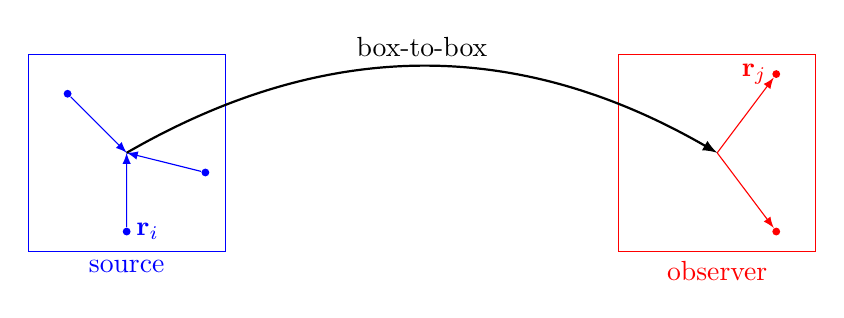
\begin{tikzpicture}[scale=2.5, >=latex]
  \draw[color=blue] (0, 0) rectangle (1, 1);
  \draw[color=red] (3, 0) rectangle (4, 1);

  \draw[color=blue] (0.2, 0.8) node[circle, fill, inner sep=1pt](s1){};
  \draw[color=blue] (0.5, 0.1) node[circle, fill, inner sep=1pt](s2){};
  \node[blue, anchor=west] at (s2) {$\vb{r}_i$};
  \draw[color=blue] (0.9, 0.4) node[circle, fill, inner sep=1pt](s3){};

  \draw[color=red] (3.8, 0.9) node[circle, fill, inner sep=1pt](o1){};
  \node[red, anchor=east] at (o1) {$\vb{r}_j$};
  \draw[color=red] (3.8, 0.1) node[circle, fill, inner sep=1pt](o2){};

  \draw[color=blue, ->] (s1) -- (0.5, 0.5);
  \draw[color=blue, ->] (s2) -- (0.5, 0.5);
  \draw[color=blue, ->] (s3) -- (0.5, 0.5);

  \draw[color=red, ->] (3.5, 0.5) -- (o1);
  \draw[color=red, ->] (3.5, 0.5) -- (o2);

  \draw[->, thick] (0.5, 0.5) to [bend left] node[pos=0.5, above]{box-to-box} (3.5, 0.5);

  \node[blue, anchor=north] at (0.5, 0) {source};
  \node[red, anchor=north] at (3.5, 0) {observer};
\end{tikzpicture}

  \end{center}
  \begin{block}{Source-to-grid, grid-to-grid, grid-to-source}
    \begin{equation*}
      \mathcal{Z}^\text{far}_{ij} = \sum_{\textcolor{red}{\vb{v}} \in C_j} \sum_{\textcolor{blue}{\vb{u}} \in C_i} \Lambda_{j\textcolor{red}{\vb{v}}} \, g(\textcolor{red}{\vb{v}}, \textcolor{blue}{\vb{u}}) \, \Lambda_{i\textcolor{blue}{\vb{u}}}
    \end{equation*}
  \end{block}
\end{frame}

\begin{frame}{Determination of the $\Lambda$s}
  \begin{block}{Multipole expansion}
    \begin{equation*}
      \underbrace{\int_{} \psi_i(\vb{r}) (x - x_0)^{m_x} (y - y_0)^{m_y} (z - z_0)^{m_z}}_{Q_{i\vb{m}}} - \sum_{\vb{u} \in C_i} \Lambda_{i \vb{u}} \underbrace{\delta(\vb{r} - \vb{u}) \dd[3]{\vb{r}}}_{W_{\vb{m}\vb{u}}} = 0
    \end{equation*}
  \end{block}
  \begin{columns}
    \column{0.7\textwidth}
      \begin{itemize}
        \item Grid discretization sufficient to recover $k_0 = \omega_0/c$ spatial variation
        \item Instantaneous ``propagation'' from source to grid
        \item Recover $\grad \div \vb{J}$ from $\grad \div Q_{i\vb{m}}$
      \end{itemize}

    \column{0.3\textwidth}
      \begin{block}{Least-squares fit}
        \begin{equation*}
          \sum_{\vb{u} \in C_i} W_{\vb{m}\vb{u}} \Lambda_{i \vb{u}} = Q_{i\vb{m}}
        \end{equation*}
      \end{block}
  \end{columns}
\end{frame}

\begin{frame}{Layered redundancies}
  \begin{center}
    Algorithmic complexity: $\displaystyle\mathcal{O}(N_t N_s^2)$
  \end{center}
  \begin{block}{Rotating-wave approximation}
    High-frequency terms barely affect dynamics; formulate equations without them.
  \end{block}
  \begin{block}{Fewer degrees-of-freedom}
    $g(\vb{r}, \vb{r}')$ has the same value at large distances; aggregate sources and transmit once.
  \end{block}
  \vphantom{
    \parbox{\linewidth}{
      \begin{block}{Imposed structure}
        $g(\vb{r}, \vb{r}') = \vb{g}(\abs{\vb{r} - \vb{r}'})$ redundant on grid; employ FFT accelerate $\oper{Z}\cdot\oper{A}$.
      \end{block}
    }
  }
  \begin{center}
    Improved algorithmic complexity: $\displaystyle\mathcal{O}\qty(\frac{N_t}{\alpha} \qty(\frac{N_s}{\beta})^2)$
  \end{center}
\end{frame}

\begin{frame}{Exploiting translational invariance}
  $g_{ij} = g(\vb{r}_i, \vb{r}_j)$ matrix becomes \emph{symmetric} and \emph{Toeplitz}\ldots
  \begin{columns}
    \column{0.5\textwidth}
      \begin{equation*}
        g = \mqty(a & b & c & d \\ b & a & b & c \\ c & b & a & c \\ d & c & b & a)
      \end{equation*}

    \column{0.5\textwidth}
      \begin{center}
        \includegraphics[width=0.5\textwidth]{figures/toep1d.pdf}
      \end{center}
  \end{columns}
  \hfill \ldots in one dimension
\end{frame}

\begin{frame}{Exploiting translational invariance}
  We can augment Toeplitz matrices to make them \emph{circulant}
  \begin{columns}
    \column{0.5\textwidth}
    \begin{equation*}
      g_a \cdot \vb{x}_a = \qty(
       \begin{array}{cccc|cccc}
         a & b & c & d & 0 & d & c & b \\
         b & a & b & c & d & 0 & d & c \\
         c & b & a & b & c & d & 0 & d \\
         d & c & b & a & b & c & d & 0 \\ \hline
         0 & d & c & b & a & b & c & d \\
         d & 0 & d & c & b & a & b & c \\
         c & d & 0 & d & c & b & a & b \\
         b & c & d & 0 & d & c & b & a \\
       \end{array}) \cdot \mqty(x_0 \\ x_1 \\ x_2 \\ x_3 \\ 0 \\ 0 \\ 0 \\ 0)
    \end{equation*}

    \column{0.5\textwidth}
      \begin{center}
        \includegraphics[width=0.6\textwidth]{figures/circ1d.pdf}
      \end{center}

  \end{columns}

  \begin{equation*}
    g_a \cdot \vb{x}_a = \overbrace{F^\dagger \big(\underbrace{D \vphantom{F \cdot \vb{x}_a}}_\text{FFT} \cdot \; (\underbrace{F \cdot \vb{x}_a)}_\text{FFT}\big)}^\text{IFFT}
  \end{equation*}
\end{frame}

\begin{frame}{Exploiting translational invariance (in three dimensions)}
  \begin{columns}
    \column{0.5\textwidth}
      \hfill \includegraphics[width=0.0875\textwidth]{figures/toep3d.pdf}
    \column{0.5\textwidth}
      \includegraphics[width=0.7\textwidth]{figures/circ3d.pdf}
  \end{columns}
\end{frame}

\begin{frame}{Layered redundancies}
  \begin{center}
    Algorithmic complexity: $\displaystyle\mathcal{O}(N_t N_s^2)$
  \end{center}
  \begin{block}{Rotating-wave approximation}
    High-frequency terms barely affect dynamics; formulate equations without them.
  \end{block}
  \begin{block}{Fewer degrees-of-freedom}
    $g(\vb{r}, \vb{r}')$ has the same value at large distances; aggregate sources and transmit once.
  \end{block}
  \begin{block}{Imposed translational invariance}
    $g(\vb{r}, \vb{r}') = \vb{g}(\abs{\vb{r} - \vb{r}'})$ redundant on grid; employ FFT to accelerate $\oper{Z}\cdot\oper{A}$.
  \end{block}
  \begin{center}
    Optimal algorithmic complexity: $\displaystyle\mathcal{O}\qty(\frac{N_t}{\alpha} N_s \log N_s)$
  \end{center}
\end{frame}

\begin{frame}{Future work}
  \begin{itemize}
    \item Additional dynamical systems (nanomagnetics, biexcitons, degenerate states)
    \item Development of isotemporal model (same basis functions for integration, interpolation)
    \item Improved $\Lambda$ weighting ($\delta$-function representation in terms of Legendre polynomials?)
    \item Multi-level FFT-based propagation
    \item Extremely large systems (MPI and/or GPU)
  \end{itemize}
\end{frame}

\section{QuEST}

\begin{frame}
  \centering
  \vspace{0.5cm}
  \includegraphics[height=\textheight]{figures/github.png}
\end{frame}

\begin{frame}
  %\begin{center}
    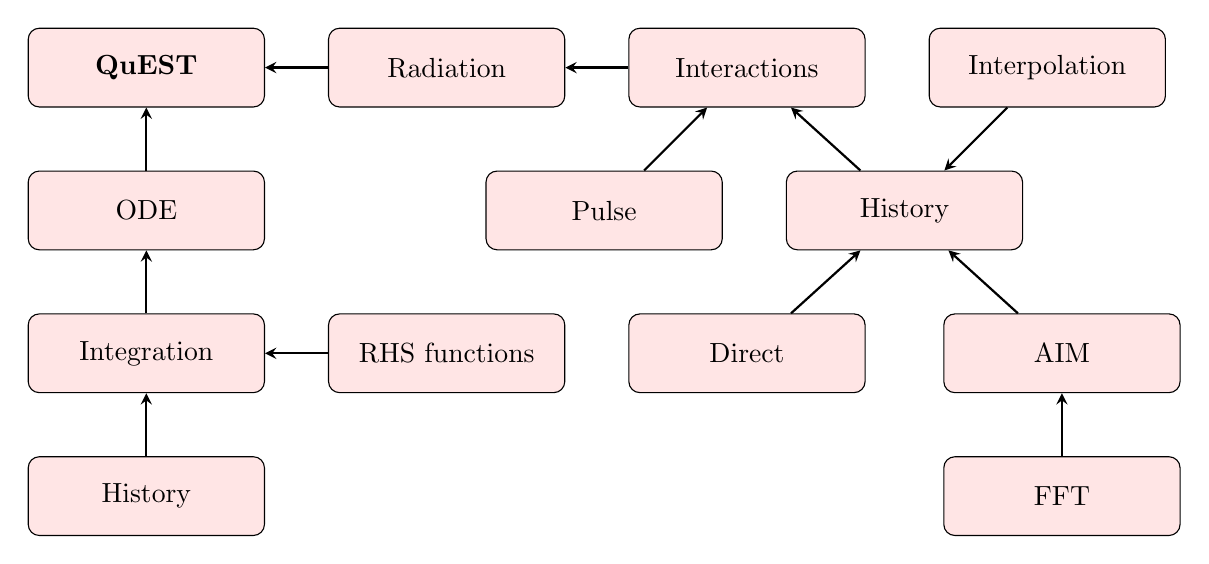
\begin{tikzpicture}[node distance=0.8cm, >=latex]
      \tikzstyle{startstop} = [rectangle, rounded corners, minimum width=3cm, minimum height=1cm,text centered, draw=black, fill=red!10]
      \tikzstyle{io} = [trapezium, trapezium left angle=70, trapezium right angle=110, minimum width=3cm, minimum height=1cm, text centered, draw=black, fill=blue!30]
      \tikzstyle{process} = [rectangle, minimum width=3cm, minimum height=1cm, text centered, draw=black, fill=orange!30]
      \tikzstyle{decision} = [diamond, minimum width=3cm, minimum height=1cm, text centered, draw=black, fill=green!30]
      \tikzstyle{arrow} = [thick,->,>=stealth]

      \node (quest) [startstop] {\textbf{QuEST}};
      \node (ode) [startstop, below= of quest] {ODE};
      \node (radiation) [startstop, right= of quest] {Radiation};

      \draw [arrow] (ode) -- (quest);
      \draw [arrow] (radiation) -- (quest);

      \node (interactions) [startstop, right= of radiation] {Interactions};
      \node (integration) [startstop, below= of ode] {Integration};
      \node (history) [startstop, below= of integration] {History};
      \node (rhs) [startstop, right= of integration] {RHS functions};

      \draw [arrow] (interactions) -- (radiation);
      \draw [arrow] (integration) -- (ode);
      \draw [arrow] (history) -- (integration);
      \draw [arrow] (rhs) -- (integration);

      \node (pulse) [startstop, below= of radiation, xshift=2cm] {Pulse};
      \node (historyI) [startstop, below= of interactions, xshift=2cm] {History};

      \draw [arrow](pulse) -- (interactions);
      \draw [arrow](historyI) -- (interactions);

      \node (interpolation) [startstop, right= of interactions] {Interpolation};
      \node (direct) [startstop, below= of historyI, xshift=-2cm] {Direct};
      \node (aim) [startstop, below= of historyI, xshift=2cm] {AIM};

      \node (fft) [startstop, below= of aim] {FFT};

      \draw [arrow] (interpolation) -- (historyI);
      \draw [arrow] (direct) -- (historyI);
      \draw [arrow] (aim) -- (historyI);
      \draw [arrow] (fft) -- (aim);

    \end{tikzpicture}
  %\end{center}
\end{frame}

\begin{frame}[standout]
  Questions?
\end{frame}

\appendix

\begin{frame}{Units}
  \begin{table}
    \begin{tabular}{lll}
      Quantity                 & Symbol            & Value                        \\ \hline \hline
      Speed of light           & $c$               & \SI{300}{\micro\meter \per \pico\second} \\
      Transition frequency     & $\omega_0$        & $\SI{1500}{\milli\eV}/\hbar$ \\
      Transition dipole moment & $\vb{d}$          & \SI{10}{\elementarycharge\bohr} (uniform) \\
      Relaxation times         & $T_{1}, T_{2}$    & \SIlist{10;20}{\pico\second} \\
      Laser frequency          & $\omega_L$        & $\SI{1500}{\milli\eV}/\hbar$ \\
      Laser wavevector         & $\vb{k}_L$        & $\omega_L/c$ ($\vb{k}_L \cdot \vb{d} = 0$) \\
      Pulse width              & $\sigma/\omega_L$ & \SI{1}{\pico\second} \\ \hline
      Integrator window        & $W$               & 20 \\
      Corrector iterations     & N/A               & max 10 (usually 4-6) \\
      Timestep                 & $\Delta t$        & \SI{0.5e-2}{\pico\second}
    \end{tabular}
  \end{table}
\end{frame}

\begin{frame}{Interpolation influence}
  \begin{columns}
    \column{0.45\textwidth}
      \begin{center}
        \includegraphics[height=0.85\textheight]{figures/spheres_of_influence}
      \end{center}

    \column{0.55\textwidth}
      \begin{itemize}
        \item Interpolate $\rho$, $\vb{P}$ due to $\abs{\vb{r} - \vb{r}'}/c \, \not \in \mathbb{N}$
        \item Sufficiently high order to recover $\partial_t^2 \vb{P}$, $\partial_t \vb{P}$, $\vb{P}$
        \item Time-domain solution imposes causality requirement: $T(t) = 0 \, \forall \, t < -1$
      \end{itemize}
  \end{columns}
\end{frame}

\end{document}
